\documentclass[UTF8]{ctexart}

\makeatletter
\def\input@path{{../../Fulcrum-Template/}{../../Operator-List/}}
\makeatother

\usepackage{FulcrumHabitCN}

\begin{document}

\tableofcontents
\newpage

	\section{实数构造}

		\subsection{序视角下的实数}

		\iffalse

			\begin{dfn}
			    []
			    {实数结构}
			    [Real Number Structure]
			    []
				结构 \((\R,+,\cdot,\leq)\) 被称为\textbf{实数结构(Real Number Structure)}, \(\R\)被称为\textbf{实数集(Set of Real Numbers)}, 其元素称为\textbf{实数(Real Number)}, 若其满足: 

				(1) \((\R,+,\cdot)\) 是一个域; 

				(2) \((\R,\leq)\) 是全序的, 且满足: 
				\[x,y,z\in\R, x\leq y\Longrightarrow x+z\leq y+z\]
				\[x\geq 0, y\geq 0\Longrightarrow xy\geq 0\]

				(3)\textbf{连续性公理}
				\[\forall X,Y\subseteq\R: (X,Y\neq\varnothing\wedge\forall x\in X, y\in Y, x\leq y), \exists c\in\R: \forall x\in X, y\in Y, x\leq c\leq y\]
			\end{dfn}

			\begin{thm}
				符合上述实数定义的结构间彼此同构. 即若 \((\R_A,+_A,\cdot_A,\leq_A)\) 与 \((\R_B,+_B,\cdot_B,\leq_B)\) 均是实数结构, 则可以构造同构 \(f:\R_A\to\R_B\), 满足: 
				\[\forall x,y\in\R_A, 
				\begin{cases}
					(1)f(x+_A y)=f(x)+_B f(y)\\
					(2)f(x\cdot_A y)=f(x)\cdot_B f(y)\\
					(3)x\leq_A y\Longrightarrow f(x)\leq_B f(y)\\
				\end{cases}\]
			\end{thm}

			证明: 

				由于 \((\R_A,+_A,\cdot_A)\) 与 \((\R_B,+_B,\cdot_B)\) 都是域, 容易证明须有: 
				\[\Longrightarrow f(0_A)=0_B, f(1_A)=1_B\]
				
				于是可以证明 \(f\) 是由 \(0_A,1_A\) 生成的子域与由 \(0_B,1_B\) 生成的子域之间的同构. 

		\fi
		
			\begin{dfn}
			    []
			    {Dedekind 切割 }
			    [Dedekind Cut]
			    []
				集合偶 \((A,B)(A,B\subsetneqq\Q)\) 称为是 \(\Q\) 的一个\textbf{Dedekind 切割}, 记作 \(A|B\), 若: 
				
				(1) \(A\) 与 \(B\) 的并铺满 \(\Q\): 
				\[A\cup B=\Q\]
				
				(2) \(A\) 与 \(B\) 的交为空: 
				\[A\cap B=\varnothing\]
				
				(3) \(A\) 中元素严格小于 \(B\) 中元素: 
				\[\forall a\in A, \forall b\in B, a<b\]
			\end{dfn}
			
			\begin{ppt}
			    []
			    {}
			    []
			    []
				对 \(A\) 中极大元 \(a=\max A\) 与 \(B\) 中极小元 \(b=\min B\) 的存在情况进行分类: 
				
				(1) \[\nexists a, \nexists b\]
				
				(2) \[\exists a, \nexists b\]
				
				(3) \[\nexists a, \exists b\]
				
				(4) \[\exists a, \exists b\]
				
				分别称为第一, 二, 三, 四类分割, 则: 

				(1) 第四类分割不存在. 

				(2) 可以建立第二, 三类分割与 \(\Q\) 间的等价关系. 
			\end{ppt}
				
			\begin{prf}
				(1)
				
				\[\exists a, \exists b\Longrightarrow a<b\]
				\[a<\frac{a+b}{2}<b, \frac{a+b}{2}\in\Q\]
				\[\frac{a+b}{2}\notin A\cup B\]
				
				与 \(A\cup B=\Q\) 矛盾. \(\square\)

				(2)
				
				构造映射 \(f:\) 全体第二类分割 \(\to\Q\) : 
				\[f(A|B):=\max A\]
				
				下证 \(\forall a\in\Q\), 有且仅有一个第二类分割满足 \(\max A=a\) : 
				
				设 \(A|B\), \(A'|B'\)是第二类分割, \(\max A=\max A'=a\). 
				\[A=A'=\{r|r\in\Q, r\leq a\}\]
				\[B=\Q-A=\Q-A'=B'\]
				\[\Longrightarrow \max A=\max A'\Longrightarrow A|B=A'|B'\]
				\[\Longrightarrow f^{-1}(a)=A|B(\max A=a, a\in\Q)\]
				
				即 \(f\) 是双射. 
				
				对于第三类分割同理. 设 \(g:\) 全体第三类分割 \(\to\Q\) 是双射, 
				
				有 \(f^{-1}\circ g:\) 全体第二类分割 \(\to\) 全体第三类分割是双射. \(\square\)
			\end{prf}
			
			\begin{dfn}
			    []
			    {实数集 }
			    [Real Number Set]
			    []
				将全体 Dedekind 切割与全体有理数集在等价关系之下的商集定义为\textbf{实数集}, 记作 \(\R\). \(\R-\Q\) 称为\textbf{无理数集 (Irrational Numbers)}

				在 Dedekind 切割构造下, 每个第二, 三类切割对应一个有理数, 每个第一类切割对应一个无理数. 

				对于实数上其他结构的构造暂略. 
			\end{dfn}

			\iffalse
			
			\begin{dfn}
				定义集合 \(\R\) 上的关系 \("\leq"\) 如下: 
				\[\forall a,b\in\R, a:=A|B,b:=A'|B'\]
				\[a\leq b\iff A\subseteq A'\]
			\end{dfn}
			
			\begin{ppt}
				\[A\subseteq A'\iff B'\subseteq B\]
			\end{ppt}
			
			证明: 
			
				\[A\subseteq A'\iff\complement_{\Q}A'\subseteq\complement_{\Q}A\iff B'\subseteq B\square\]
			
			\begin{ppt}
				上述 \("\leq"\) 关系是一种偏序关系. 
			\end{ppt}
			
			证明: 
			
				(1)自反性: 
				\[\forall x=A|B\in\R, A\subseteq A, B\subseteq B\Longrightarrow x\leq x\]
				
				(2)反互逆性: 
				\[\forall x=A|B, y=A'|B': x\leq y, y\leq x\]
				\[A\subseteq A', A'\subseteq A\Longrightarrow A=A'\Longrightarrow x=y\]
				
				(3)传递性: 
				\[\forall x=A|B, y=A'|B', z=A''|B'': x\leq y, y\leq z\]
				\[A\subseteq A', A'\subseteq A''\Longrightarrow A\subseteq A''\Longrightarrow x\leq z\square\]
			
			\begin{dfn}
				定义广义的有理数及有理数集之间的加法运算: 
				\[\forall r\in\Q, A\subseteq\Q, r+A:=A+r:=\{r+a|a\in A\}\]
				\[\forall A,B\subseteq\Q, A+B:=\{a+b|a\in A, b\in B\}\]
			\end{dfn}
			
			\begin{ppt}
				\[\forall x=A|B,y=A'|B'\in(\R-\Q), \]
				\[|\Q-((A+A')\cup(B+B'))|\in\{0,1\}\]
			\end{ppt}
			
			证明: 
			
				运用反证法. 
				
				假设 \(\exists x,y\in\Q: x<y, x,y\notin (A+A')\cup(B+B')\), 则: 
				
				\begin{lma}
					\[\forall x,y\in\Q: x<y, \exists a\in A, b\in B: b-a=y-x\]
				\end{lma}
				
				证明: 
					
					\[\forall p\in A, q\in B, q-p\in\Q\]
					\[n:=[\frac{q-p}{y-x}]+1, p+n(y-x)>q, \Longrightarrow p+n(y-x)\in B\]
					
					考虑有理数列 \(\{p_i|p_i=p+i(y-x), 0\leq i\leq n\}\), 有: 
					\[p_0=p\in A, p_n=p+n(y-x)\in B\]
					
					必 \(\exists\) 相邻的两项 \(p_i, p_{i+1}: p_i\in A, p_{i+1}\in B\). 
					
					否则, 任意两项在同一集合内可归纳推出 \(\{p_i\}\subseteq A\) 或 \(B\), 矛盾. 
					
					其中, \(a:=p_i, b:=p_{i+1}\), 有 \(a\in A, b\in B, b-a=y-x\). \(\square\)
					\[\forall a\in A, x-a\notin A', \Longrightarrow x-a\in(\Q-A')=B'\]
			
					取满足引理条件的 \(a,b\), 则: 
					\[y=x+(y-x)=a+(x-a)+(y-x)=b+(x-a)\]
			
					其中 \(b\in B, x-a\in B'\), 与 \(y\notin B+B'\) 矛盾. 
					\[\Longrightarrow|\Q-((A+A')\cup(B+B'))|\in\{0,1\}\square\]
			
			\begin{ppt}
				若 \(|\Q-((A+A')\cup(B+B'))|=1, \exists\) 唯一的有理数 \(r\in\Q\) : 
				\[\forall a\in A, a'\in A', r>a+a'; \] 
				\[\forall b\in B, b'\in B', r<b+b'; \]
			\end{ppt}
			
			证明: 
			
				运用反证法. 
			
				考虑 \(r\) 为 \(\Q-((A+A')\cup(B+B'))\) 中唯一的元素. 
				
				假设 \(\exists a\in A, a'\in A': r<a+a'\), 
				\[r-a<a', \Longrightarrow r-a\in A', \Longrightarrow r=a+(r-a)\in A+A'\]
				
				矛盾. 
				\[\Longrightarrow\forall a\in A, a'\in A', r>a+a'\]
				
				同理可证 \(\forall b\in B, b'\in B', r<b+b'\). \(\square\)
				
			\begin{dfn}
				定义实数集上的加法为二元运算 \("+": \R\times\R\to\R\) : 
				\[\forall x=A|B, y=A'|B'\in\R, \]
				\[x+y:=
				\begin{cases}
				x+y & , x,y\in\Q\\
				(A+y)|(B+y) & , y\in\Q, x\in(\R-\Q)\\
				(x+A')|(x+B') & , x\in\Q, y\in(\R-\Q)\\
				f((A+A',B+B')) & , x,y\in(\R-\Q), 
				\end{cases}\]
				
				其中\[f((A+A',B+B'))=
				\begin{cases}
					(A+A')|(B+B') & , |\Q-((A+A')\cup(B+B'))|=0\mbox{(即 \(x+y\) 为无理数)}\\
					r & , |\Q-((A+A')\cup(B+B'))|=1\mbox{(即 \(x+y\) 为有理数)}
				\end{cases}\]
				
				其中 \(r\) 为 \(\Q-((A+A')\cup(B+B'))\) 中唯一的元素. 
			\end{dfn}

			\fi
			
			\begin{dfn}
			    []
			    {扩充实数集 }
			    [Extended Real Number Set]
			    []
			{}
			{负无穷大(Negative Inifinity)}
			{}
			{}
				定义囊括了正负无穷大的实数集为\textbf{扩充实数集} \(\bar\R\) : 
				\[\bar\R:=\R\cup\{+\infty,-\infty\}\]

				\iffalse

				规定 \(\bar\R\) 内的广义四则运算如下: 
				\[\begin{cases}
					\forall x\in\R, x+(+\infty)=x-(-\infty)=+\infty\\
					\forall x\in\R, x+(-\infty)=x-(+\infty)=-\infty\\
					(+\infty)+(+\infty)=(+\infty)-(-\infty)=+\infty\\
					(-\infty)+(-\infty)=(-\infty)-(+\infty)=-\infty\\
				\end{cases}\]
				\[\begin{cases}
					\forall x\in\R^+, x\cdot(+\infty)=x-(-\infty)=+\infty\\
					\forall x\in\R, x+(-\infty)=x-(+\infty)=-\infty\\
					(+\infty)+(+\infty)=(+\infty)-(-\infty)=+\infty\\
					(-\infty)+(-\infty)=(-\infty)-(+\infty)=-\infty\\
				\end{cases}\]

				\fi
			\end{dfn}
		
			\begin{thm}
			    []
			    {确界存在定理}
			    []
			    []
				由 Dedekind 切割得到的实数集是完备偏序的. 
			\end{thm}

			\begin{prf}

			\end{prf}
			
			\begin{thm}
			    []
			    {单调有界数列收敛定理}
			    []
			    []
				单调有界数列收敛: 
				\[\forall\{a_n\}(\forall n\in\N^*, a_n\leq a_{n+1}\wedge\exists M\in\R, \forall n\in\N^*, a_n\leq M), \exists a\in\R, \lim_{n\to+\infty}a_n=a\] 
				\[\forall\{b_n\}(\forall n\in\N^*, b_n\geq b_{n+1}\wedge\exists m\in\R, \forall n\in\N^*, b_n\leq m), \exists b\in\R, \lim_{n\to+\infty}b_n=b\]
			\end{thm}
			
			\begin{prf}
				
			\end{prf}
			
			\begin{thm}
			    []
			    {Cauchy-Cantor 闭区间套定理}
			    []
			    []
				设 \(\{a_n\},\{b_n\}\) 是实数序列, 满足: 
				
				\(\{a_n\}\) 单调增, \(\{b_n\}\) 单调减, 且 \(\{a_n\}\) 各项小于等于 \(\{b_n\}\) 各项: 
				\[\forall n\in\N^*, a_n\leq a_{n+1}\leq b_{n+1}\leq b_n\]
				\[(\text{即} [a_{n+1},b_{n+1}]\subseteq[a_n,b_n])\]

				则: 
				
				(1) 存在介于两数列之间的数: 
				\[\exists C\in\R, \forall n\in\N^*, a_n\leq C\leq b_n\]
				\[\left(\text{即} \bigcap_{n=1}^{+\infty}[a_n,b_n]\neq\varnothing\right)\]

				(2) \(\{a_n\}, \{b_n\}\)收敛: 
				\[\exists a,b\in\R: \lim_{n\to+\infty}a_n=a,\lim_{n\to+\infty}b_n=b\]
				
				进一步地, 若 \(\{a_n\}\) 与 \(\{b_n\}\) 可以无限靠近: 
				\[\lim_{n\to+\infty}d(a_n,b_n)=0\]

				则: 
				
				(1) 介于两数列间的数唯一: 
				\[\exists\text{ 唯一的 }C\in\R, \forall n\in\N^*, a_n\leq C\leq b_n\]
				\[\left(\text{即 }\bigcap_{n=1}^{+\infty}[a_n,b_n]=\{C\}\right)\]

				(2) 两数列极限相等, 且为 \(C\): 
				\[\lim_{n\to+\infty}a_n=\lim_{n\to+\infty}b_n=C\]
			\end{thm}
			
			\begin{prf}
				
			\end{prf}

		\subsection{度量空间视角下的实数}

			\begin{dfn}
			    []
			    {实数集 }
			    [Real Number Set]
			    []
				对 \(\Q\) 上的全体 Cauchy 列建立等价关系: 若将两数列合并后仍为 Cauchy 列, 则认为它们等价. 

				将全体 Cauchy 列关于该等价关系的商集定义为实数集. 
			\end{dfn}
			
			\begin{thm}
			    []
			    {Cauchy收敛定理}
			    []
			    []
				在实数集中任意Cauchy列收敛. 
			\end{thm}

		\subsection{通常拓扑视角下的实数}
			
			\begin{dfn}
			    []
			    {通常拓扑 }
			    [Regular Topology]
			    []
				由实数上的一般度量 \(d(x,y)=|x-y|\) 诱导得到的拓扑称为实数上的\textbf{通常拓扑}: 
				\[\T=\{X\in\PP(\R)|\forall x\in X, \exists\delta\in\R^+, \Ball{x}{\delta}\subseteq X\}\]
			\end{dfn}
			
			\begin{thm}
			    []
			    {开集结构定理}
			    []
			    []
				通常拓扑下的开集恰是全体有限个或可数个开区间的无交并: 
				\[\forall O\in \T, \exists\{(a_n,b_n)\}(\forall n\in\N^*, b_n<a_{n+1}), O=\bigcup_{i=1}^n(a_i,b_i)(n\in\N\cup\{+\infty\})\]
			\end{thm}
			
			\begin{prf}
				证明有限个或可数个开区间的无交并是开集是容易的: 开区间是开集, 于是开区间的任意并都是开集. 

				现证明任何开集都能表示成有限个或可数个开区间的无交并: 

				考虑全体有理数. 对于开集内的有理数, 考虑其向一侧``伸展''的最大长度. 再证明任何两个有理数``伸展''得到的开区间要么相同, 要么不相交. 于是可以写出由全体有理数``伸展''得到的开区间的无交并, 它是原开集的一个子集. 
				
				现在只需证明它就是开集本身. 假设开集中仍有未被上述集合囊括的元素, 那么其一定是无理数, 它必有一个开邻域包含于原开集. 这个开邻域中必然有有理数, 于是这个无理数也必然包含于某一个有理数``伸展''得到的开区间内, 矛盾. \(\square\)
			\end{prf}
			
			\begin{crl}
			    []
			    {闭集结构定理}
			    []
			    []
				通常拓扑下的闭集必能表示为有限个或可数个闭区间或单点集的无交并. 
			\end{crl}
			
			\begin{prf}
				闭集是补集是开集, 先将开集表示为有限个或可数个开区间的并, 再取出区间各端点即可用单点集与闭集的有限或可数并表示闭集. \(\square\)
			\end{prf}
				
			\begin{thm}
			    []
			    {Heine-Borel 有限开覆盖定理}
			    []
			    []
				\(\R\) 上有界闭集的任何开集覆盖有有限子覆盖: 
				\[\]

				该定理拓扑形式的广义结论: Hausdorff 空间上的紧集与有界闭集等价. 
			\end{thm}
		
        \section{实数列}
  
            \subsection{数列极限}
			
			\begin{dfn}
			    []
			    {数列极限}
			    [Limit of a Sequence]
			    []
				一个实数序列 \(\{a_n\}\) 称为是\textbf{收敛(Converge)}的, 若: 
				\[\exists a\in \R, \forall \varepsilon\in\R^+, \exists N\in\mathbb{Z}^+, \forall n>N, a_n\in\mathcal{B}(a,\varepsilon)\]
				
				其中常数 \(a\) 称为数列 \(\{a_n\}\) 在 \(n\to+\infty\) 处的\textbf{极限(limit)}, 记作: 
				\[\lim_{n\to+\infty}a_n=a\]
				
				实数序列 \(\{a_n\}\) 称为是\textbf{发散(Diverge)}的, 若: 
				\[\nexists\lim_{n\to+\infty}a_n\]
			\end{dfn}
			
			\begin{ppt}
			    []
			    {收敛数列的极限唯一}
			    []
			    []
				\[\lim_{n\to+\infty}a_n=a, \lim_{n\to+\infty}a_n=a'\Longrightarrow a=a'\]
			\end{ppt}
			
			\begin{prf}
				\[\because\lim_{n\to+\infty}a_n=a, \lim_{n\to+\infty}a_n=a'\]
				\[\Longrightarrow\forall\varepsilon\in\R^+, \exists N\in\mathbb{Z}^+: \forall n>N, a_n\in U(a,\varepsilon), a_n\in U(a',\varepsilon)\]
				\[\varepsilon:=\frac{|a-a'|}{2}>0\Longrightarrow U(a,\varepsilon)\cap U(a',\varepsilon)=\varnothing\]
				
				与 \(\forall n>N, a_n\in U(a,\varepsilon)\cap U(a',\varepsilon)\) 矛盾. \(\square\)
                \end{prf}
				
			\begin{ppt}
			    []
			    {数列极限的四则运算}
			    []
			    []
				设 \(\lim\limits_{n\to+\infty}a_n=A, \lim\limits_{n\to+\infty}b_n=B\), 则: 
                \[\lim\limits_{n\to+\infty}(a_n+b_n)=A+B\]
                \[\lim\limits_{n\to+\infty}(a_n\cdot b_n)=A\cdot B\]

                若 \(B\neq 0\), 则: 
                \[\lim\limits_{n\to+\infty}(\frac{a_n}{b_n})=\frac{A}{B}\]
			\end{ppt}
			
			\begin{ppt}
			    []
			    {收敛数列有界性}
			    []
			    []
				内容: 
				\[\lim_{n\to+\infty}a_n=a\in\R\Longrightarrow\exists m,M\in\R: \forall n\in\mathbb{Z}^+, m\leq a_n\leq M\]
			\end{ppt}
			
			\begin{prf}
				\[\lim_{n\to+\infty}a_n=a\Longrightarrow\forall\varepsilon\in\R^+, \exists N\in\mathbb{Z}^+: \forall n>N, a_n\in U(a,\varepsilon)\]
				\[m:=\min(\min_{1\leq n\leq N}(\{a_n\}),a-\varepsilon)\]
				\[M:=\max(\max_{1\leq n\leq N}(\{a_n\}),a+\varepsilon)\square\]
                \end{prf}
   
			\begin{ppt}
			    []
			    {收敛数列保序性}
			    []
			    []
				内容: 
				\[\lim_{n\to+\infty}a_n=a>b=\lim_{n\to+\infty}b_n\Longrightarrow\exists N\in\mathbb{Z}^+: \forall n>N, a_n>b_n\]
				\[\lim_{n\to+\infty}a_n=a\geq b=\lim_{n\to+\infty}b_n\impliedby\exists N\in\mathbb{Z}^+: \forall n>N, a_n>b_n\]
			\end{ppt}
			
			\begin{prf}
                (1) 充分性: 
   
				\[\lim_{n\to+\infty}a_n=a,\lim_{n\to+\infty}b_n=b\Longrightarrow\forall\varepsilon\in\R^+, \exists N\in\mathbb{Z}^+: \forall n>N, a_n\in U(a,\varepsilon), b_n\in U(b,\varepsilon)\]
				
				取\(\varepsilon=\frac{a-b}{2}\)
				
				\[\Longrightarrow\exists N\in\mathbb{Z}^+: \forall n>N, a_n>\frac{a+b}{2}>b_n\square\]

				(2) 必要性: 

				不妨设a<b, 由前反证. \(\square\)
            \end{prf}
			
			\begin{ppt}
			    []
			    {夹逼定理 }
			    [Sandwich Theorem]
			    []
                内容: 
                \[\lim_{n\to+\infty}a_n=\lim_{n\to+\infty}b_n=a(a\in\R\cup\{+\infty,-\infty\})\]
				\[\exists N\in\mathbb{Z}^+: \forall n>N, a_n\leq c_n\leq b_n\Longrightarrow\lim_{n\to+\infty}c_n=a\]
			\end{ppt}
			
			\begin{prf}
				\[\lim_{n\to+\infty}a_n=\lim_{n\to+\infty}b_n=a\Longrightarrow\forall\varepsilon\in\R^+, \exists N'\in\mathbb{Z}^+: \forall n>N', a_n,b_n\in U(a,\varepsilon)\]
				\[N'':=\max(N,N')\]
				\[\forall n>N'', c_n\in[a_n,b_n]\subseteq U(a,\varepsilon)\]
            \end{prf}
			
	\iffalse
 
		\subsection{实数完备性定理}
			
			\begin{thm}
				单调有界数列收敛. 
			\end{thm}
				
			\begin{prf}
				We prove the special case where \(a_n\) is monotonically increasing and bounded above, and we can prove the rest of the cases in the same way. 

				We prove the proposition by contradiction. 
				
				We first make the hypothesis that \(a_n\) diverges, so that: 
				\[\forall a\in\R, \exists\varepsilon\in\R^+(\forall N\in\N, \exists n>N(a_n\notin U(a,\varepsilon)))\]
		
				Let \(a=\sup\{a_n\}\), then \(\exists\varepsilon\in\R^+(\forall N\in\N, \exists n>N(a_n\notin U(\sup\{a_n\},\varepsilon)))\)
				\[a_n\notin U(\sup\{a_n\},\varepsilon)\Longrightarrow a_n<\sup\{a_n\}-\varepsilon\]
		
				This is because \(a_n<\sup\{a_n\}\), so that if any term of \(\{a_n\}\) falls inside the \(\varepsilon\)-neighbourhood of \(\sup\{a_n\}\), all subsequent terms will also fall inside that neighbourhood due to the monotonicity of \(\{a_n\}\), which contradicts with the conclusion above. 
		
				So that we have found another upper bound \(\sup\{a_n\}-\varepsilon\) for \(\{a_n\}\) that is smaller than \(\sup\{a_n\}\), contradition. \(\square\)
			\end{prf}
			
			\begin{thm}
			    []
			    {Bolzano-Weiestrass定理}
			    []
			    []
				有界数列有收敛子列. 
			\end{thm}
			
			
			\begin{prf}
				设 \(\{a_n\}\) 是任意有界数列, \(m:=\inf(a_n),n:=\sup(a_n)\). 
				
				构造 \(a_n\) 的两个子列: \[\{a_{1,n}\},\{a_{2,n}\}: a_{1,n}\in[m,\frac{m+n}{2}],a_{2,n}\in[\frac{m+n}{2},n]\]
			\end{prf}

			\begin{thm}
			    []
			    {Cauchy-Cantor闭区间套定理}
			    []
			    []
				一个闭区间序列 \(\{X_i|X_i\text{是闭区间}, i\in\N\}\) 被称为是\textbf{闭区间套}, 若其满足: 
				\[\forall i\in\N, X_{i+1}\subseteq X_i\]

				对于该闭区间套, 有: \(\exists c\in\R: \forall i\in\N, c\in X_i\), 且: 
				\[\forall\varepsilon>0, \exists i\in\N: |X_i|<\varepsilon\Longrightarrow\text{这样的 \(c\) 是唯一的. }\]
			\end{thm}
			
			\begin{thm}
			    []
			    {Borel-Lebesgue原理/Heine-Borel有限开覆盖定理}
			    []
			    []
				称一个集族 \(S=\{X_i|i\in I\}\) \textbf{覆盖}集合 \(Y\), 若 \(Y\subseteq\bigcup\limits_{i\in I}X_i\). 

				\(\forall\)覆盖 \(Y\) 的开区间族 \(S=\{X_i|i\in I\}\), \(\exists S\)的有限子集族 \(S'=\{X_j|j\in J, J\text{是有限集}\}\subseteq S: S'\) 能覆盖 \(Y\). 

			\end{thm}

        \fi
   
		\subsection{发散数列}

			\begin{dfn}
			    []
			    {}
			    []
			    []
				对于给定的点 \(P\) 和点集 \(S\) \textbf{聚点(Accumulation Point)},若其满足: 
				
				\[\forall\varepsilon, \exists\{x_n\}, \forall i\in \mathbb{N^*}, x_i\in \mathbb{S}, x_i\in U_{\varepsilon}(\dot{P})\]

				即, 对于P的任意小邻域 \(U(P)\) , 都存在无限多个属于 \(S\) 且不等于 \(P\) 的点在 \(U(P)\) 内
			\end{dfn}

			\begin{ppt}
			    []
			    {}
			    []
			    []
				任意数列存在至少一个聚点

				由Bolzano-Weiestrass定理可得
			\end{ppt}

			\begin{dfn}
			    []
			    {上 / 下极限}
			    [Upper / Lower Limit]
			    []
			\end{dfn}

			\begin{ppt}
			    []
			    {}
			    []
			    []
				内容: 
				\[\varliminf_{n\to\infty}x_n+\varliminf_{n\to\infty}y_n\leq\varliminf_{n\to\infty}\left(x_n+y_n\right)\leq\varliminf_{x\to\infty}x_n+\varlimsup_{x\to\infty}y_n\eqno{(1)}\]
				\[\varliminf_{n\to\infty}x_n+\varlimsup_{n\to\infty}y_n\leq\varlimsup_{n\to\infty}\left(x_n+y_n\right)\leq\varlimsup_{x\to\infty}x_n+\varlimsup_{x\to\infty}y_n\eqno{(2)}\]
				\[\varliminf_{n\to\infty}x_n\cdot\varliminf_{n\to\infty}y_n\leq\varliminf_{n\to\infty}\left(x_ny_n\right)\leq\varliminf_{x\to\infty}x_n\cdot\varlimsup_{x\to\infty}y_n\eqno{(3)}\]
				\[\varliminf_{n\to\infty}x_n\cdot\varlimsup_{n\to\infty}y_n\leq\varlimsup_{n\to\infty}\left(x_ny_n\right)\leq\varlimsup_{x\to\infty}x_n\cdot\varlimsup_{x\to\infty}y_n\eqno{(4)}\]
			\end{ppt}
		
		\subsection{无穷大量和无穷小量}
			
			\begin{dfn}
			    []
			    {}
			    []
			    []
				数列 \(\{a_n\}\) 称为是一个\textbf{正无穷大量(Positive Infinity)}, 若: 
				\[\forall M\in\R^+, \exists N\in\mathbb{Z}^+: \forall n>N, a_n>M\]
				
				记作\[\lim_{n\to+\infty}a_n=+\infty\]
				
				数列 \(\{a_n\}\) 称为是一个\textbf{负无穷大量(Negative Infinity)}, 若: 
				\[\forall M\in\R^+, \exists N\in\mathbb{Z}^+: \forall n>N, a_n<-M\]
				
				记作\[\lim_{n\to+\infty}a_n=-\infty\]
				
				数列 \(\{a_n\}\) 称为是一个\textbf{无穷大量(Infinity)}, 若: 
				\[\forall M\in\R^+, \exists N\in\mathbb{Z}^+: \forall n>N, |a_n|>M\]
				
				记作\[\lim_{n\to+\infty}a_n=\infty\]
				
				数列 \(\{a_n\}\) 称为是一个\textbf{无穷小量(Infinitesimal)}, 若: 
				\[\lim_{n\to+\infty}a_n=0\]
			\end{dfn}
			
			\begin{ppt}
			    []
			    {}
			    []
			    []
				涉及无穷大量的四则运算法则部分适用: 
			\end{ppt}
			
			\begin{dfn}
			    []
			    {}
			    []
			    []
				无穷大量 \(\{a_n\}\) 称为是 \(\{b_n\}\) 的\textbf{高阶无穷大量}, 若: 
				\[\lim_{n\to+\infty}\frac{a_n}{b_n}=\infty\vee\lim_{n\to+\infty}\frac{b_n}{a_n}=0\]
				
				无穷大量 \(\{a_n\}\) 称为是 \(\{b_n\}\) 的\textbf{低阶无穷大量}, 若: 
				\[\lim_{n\to+\infty}\frac{b_n}{a_n}=\infty\vee\lim_{n\to+\infty}\frac{a_n}{b_n}=0\]
			
				无穷大量 \(\{a_n\}\) 称为是 \(\{b_n\}\) 的\textbf{同阶无穷大量}, 若: 
				\[\lim_{n\to+\infty}\frac{a_n}{b_n}=c\in(\R-\{0\})\]
				
				无穷大量 \(\{a_n\}\) 称为是 \(\{b_n\}\) 的\textbf{等价无穷大量}, 若: \[\lim_{n\to+\infty}\frac{a_n}{b_n}=1\]
				
				记为 \(a_n\sim b_n\). 
								
				无穷小量 \(\{a_n\}\) 称为是 \(\{b_n\}\) 的\textbf{高阶无穷小量}, 若: 
				\[\lim_{n\to+\infty}\frac{a_n}{b_n}=0\vee\lim_{n\to+\infty}\frac{b_n}{a_n}=\infty\]
				
				记为 \(a_n=o(b_n)\). 
				
				无穷小量 \(\{a_n\}\) 称为是 \(\{b_n\}\) 的\textbf{低阶无穷小量}, 若: 
				\[\lim_{n\to+\infty}\frac{b_n}{a_n}=\infty\vee\lim_{n\to+\infty}\frac{b_n}{a_n}=0\]
				
				记为 \(b_n=o(a_n)\). 
			
				无穷小量 \(\{a_n\}\) 称为是 \(\{b_n\}\) 的\textbf{同阶无穷小量}, 若: 
				\[\lim_{n\to+\infty}\frac{a_n}{b_n}=c\in(\R-\{0\})\]
				
				无穷小量 \(\{a_n\}\) 称为是 \(\{b_n\}\) 的\textbf{等价无穷小量}, 若: 
				\[\lim_{n\to+\infty}\frac{a_n}{b_n}=1\]	
				
				记为 \(a_n\sim b_n\). 
				
			\end{dfn}
			
			\begin{ppt}
			    []
			    {}
			    []
			    []
				同阶无穷大/小量关系与等价无穷大/小量关系是等价关系. 
			\end{ppt}
		
		\subsection{待定型极限}
			
			\begin{thm}
			    []
			    {Stolz-Cesaro定理}
			    []
			    []
				内容: 
				\[S_n:=\sum_{i=1}^n a_i
				\qquad
				T_n:=\sum_{i=1}^n b_i
				\qquad
				b_i\neq 0\]
			
				那么在以下情况下: (其余部分情况可转化为下列情况)

				(1) \(\dfrac{*}{\infty}\) 型: 
				\(\lim\limits_{n\to+\infty}T_n=+\infty\)且\(b_n>0\)

				(2) \(\dfrac{0}{0}\) 型: 
				\(\lim\limits_{n\to+\infty}T_n=0,\lim\limits_{n\to+\infty}S_n=0\)且\(,b_n<0(n>1)\)
				
				有: 

				\[\lim_{n\to+\infty}\frac{S_n}{T_n}=\lim_{n\to+\infty}\frac{a_n}{b_n}\]
			\end{thm}
			
			\begin{prf}
				证明( \(\dfrac{*}{\infty}\) 型): 
				
					由极限定义: 
					\[\lim_{n\to+\infty}\frac{a_n}{b_n}=k\iff\forall\varepsilon\in\R^+, \exists N\in\N(\forall n>N, \frac{a_n}{b_n}\in(k-\varepsilon,k+\varepsilon))\]
					\[\overset{n>N}{\Longrightarrow}a_n\in((k-\varepsilon)b_n,(k+\varepsilon)b_n)\]
	
					\[\sum_{i=1}^N a_i:=A_N,\sum_{i=1}^N b_i:=B_N\]
					\[S_n:=\sum_{i=1}^n a_i=\sum_{i=1}^N a_i+\sum_{i=N+1}^n a_i\]
					\[\Longrightarrow S_n\in\left(A_N+(k-\varepsilon)\sum_{n=N+1}^n b_n,A_N+(k+\varepsilon)\sum_{n=N+1}^n b_n\right)\]
					\[\iff S_n\in(A_N+(k-\varepsilon)(T_n-B_N),A_N+(k+\varepsilon)(T_n-B_N))\]
	
					\[\overset{T_n>0}{\Longrightarrow}\frac{S_n}{T_n}\in\left(\frac{A_N-(k-\varepsilon)B_N}{T_n}+(k-\varepsilon),\frac{A_N-(k+\varepsilon)B_N}{T_n}+(k+\varepsilon)\right)\]
					取 \(N'\) 使\(T_n>2B_N\)
					\[\therefore\frac{S_n}{T_n}\in\left(k-2\varepsilon,k+2\varepsilon\right)\]
	
				证明( \(\dfrac{0}{0}\) 型): 
	
					易证, \(\frac{a_1}{b_1}\leq\frac{a_2}{b_2}\) 且 \(b_1,\ b_2>0\) 时, 不等式 \(\frac{a_1}{b_1}\leq\frac{a_1+a_2}{b_1+b_2}\leq\frac{a_2}{b_2}\) 恒成立.
					
					由定义
					\[\lim_{n\to+\infty}\frac{a_n}{b_n}=k\iff\forall\varepsilon\in\R^+, \exists N\in\N(\forall n>N, \frac{a_n}{b_n}\in(k-\varepsilon,k+\varepsilon))\]
					归纳得, 当 \(b_i>0,i\in\Z\) 时
					\[\frac{S_n-S_N}{T_n-T_N}\in\left(k-\varepsilon,k+\varepsilon\right), N<n\]
					
					由 \(\lim\limits_{n\to+\infty}T_n\lim\limits_{n\to+\infty}S_n=0\),再令N足够大
	
					既证
			\end{prf}

			\iffalse
			
				\[\lim_{n\to+\infty}\frac{S_n}{T_n}=k\iff\forall\varepsilon\in\R^+, \exists N\in\N(\forall n>N, \frac{S_n}{T_n}\in(k-\varepsilon,k+\varepsilon))\]
				\[\overset{n>N}{\Longrightarrow}S_n\in((k-\varepsilon)T_n,(k+\varepsilon)T_n)\]
				\[\overset{n>N+1}{\Longrightarrow}a_n=S_n-S_{n-1}\in((k-\varepsilon)T_n-(k+\varepsilon)T_{n-1},(k+\varepsilon)T_n-(k-\varepsilon)T_{n-1})\]
				\[=((k-\varepsilon)(T_n-T_{n-1})-2\varepsilon T_{n-1},(k+\varepsilon)(T_n-T_{n-1})+2\varepsilon T_{n-1})\]
				\[=((k-\varepsilon)b_n-2\varepsilon T_{n-1},(k+\varepsilon)b_n+2\varepsilon T_{n-1})\]
				\[\overset{b_n>0}{\Longrightarrow}\frac{a_n}{b_n}\in\left((k-\varepsilon)-\frac{2\varepsilon T_{n-1}}{b_n},(k+\varepsilon)+\frac{2\varepsilon T_{n-1}}{b_n}\right)\]	
			
			\fi

		\subsection{常用重要极限}
		
			\begin{thm}
			    []
			    {}
			    []
			    []
				内容: 
				\[\lim_{n\to+\infty}\left(1+\frac{1}{n}\right)^n\text{ 收敛}\]
			\end{thm}

                \begin{prf}
                    \[e_n:={\left(1+\frac{1}{n}\right)}^n\]
                
                    运用单调有界数列收敛定理: 

                    (1) 证明 \(e_n\) 单调增: 
                        \[e_n
                        ={\left(1+\frac{1}{n}\right)}^n
                        \leq{\left(1+\frac{1}{n+1}\right)}^{n+1}
                        =e_{n+1}\]
    
                        由基本不等式知: 
                        \[{\left(1+\frac{1}{n}\right)}^n\times 1
                        \leq{\left(\frac{n\times\left(1+\frac{1}{n}\right)+1}{n+1}\right)}^{n+1}
                        ={\left(1+\frac{1}{n+1}\right)}^{n+1}\]

                    (2) 证明 \(e_n\) 有上界: 
                        \[e_n={\left(1+\frac{1}{n}\right)}^n
                        \leq{\left(1+\frac{1}{n}\right)}^{n+1}
                        =\frac{1}{{\left(1-\frac{1}{n+1}\right)}^{n+1}}\]

                        注意到 \({\left(1-\frac{1}{n+1}\right)}^{n+1}\) 可与 (1) 同理证明是单调减的, 于是上式右式单调增. 
                        \[\Longrightarrow e_n\leq{\left(1+\frac{1}{1}\right)}^{1+1}=4\square\]
                \end{prf}

			\begin{dfn}
			    []
			    {}
			    []
			    []
				上述极限值称为\textbf{自然常数(Natural Constant)}或\textbf{Napier常数(Napier's Constant)}, 记为 \(e\). 
			\end{dfn}

                \iffalse

				\[e_n:=\left(1+\frac{1}{n}\right)^n=\sum_{i=0}^n C_n^i\frac{1}{n^i}=\sum_{i=0}^n\frac{n!}{i!(n-i)!}\cdot\frac{1}{n^i}=\sum_{i=0}^n\left(\frac{1}{i!}\prod_{j=0}^{i-1}\frac{n-j}{n}\right)\]
				\[\Downarrow\]
				\[\begin{cases}
					\begin{array}{rcllllll}
						e_n & = & 2 + \frac{1}{2!}\left(1-\frac{1}{n}\right) & + \frac{1}{3!}\left(1-\frac{1}{n}\right)\left(1-\frac{2}{n}\right) & +\cdots+ \frac{1}{n!}\left(1-\frac{1}{n}\right)\cdots\left(1-\frac{n-1}{n}\right)\\
						e_{n+1} & = & 2 + \frac{1}{2!}\left(1-\frac{1}{n+1}\right) & + \frac{1}{3!}\left(1-\frac{1}{n+1}\right)\left(1-\frac{2}{n+1}\right) & +\cdots+ \frac{1}{n!}\left(1-\frac{1}{n+1}\right)\cdots\left(1-\frac{n-1}{n+1}\right)\\
						& & + d_n
					\end{array}
				\end{cases}\]	
				\[\left(d_n=\frac{1}{(n+1)!}\left(1-\frac{1}{n+1}\right)\cdots\left(1-\frac{n}{n+1}\right)\right)\]
				\[\Longrightarrow e_{n+1}>e_n\]
				
				即 \(e_n\) 严格增. 
				\[S_n:=\sum_{i=0}^n\frac{1}{i!}\qquad(0!:=1)\]
				\[\Longrightarrow e_n<S_n<1+\sum_{i=0}^n\frac{1}{2^{i-1}}=3-\frac{1}{2^{n-1}}\]

				即 \(e_n\) 有上界, 故 \(e_n\) 有极限. \(\square\)

                \fi
			
			\begin{thm}
			    []
			    {}
			    []
			    []
				\(e\)的估计: 
				\[\forall m\in\N, \exists n\in\N(S_m\leq e_n\leq S_n)\]
			\end{thm}

			证明: 

				右侧显然. 
			
			\begin{thm}
			    []
			    {}
			    []
			    []
				\(e\)是无理数. 
			\end{thm}

			\begin{prf}
				运用反证法. 
				
				假设 \(e\) 是有理数, 则可设: 
				\[e=1+\frac{1}{2!}+\frac{1}{3!}+\cdots:=\frac{q}{p}\quad(p,q\in\mathbb{N}^*)\]
				\[\Longrightarrow p!+\frac{p!}{2!}+\cdots+\frac{p!}{p!}+\frac{p!}{(p+1)!}+\cdots=q(p-1)!\]
				\[\forall k=1,2,\cdots,p,\Longrightarrow k!|p!\]
				\[p!+\frac{p!}{2!}+\cdots+\frac{p!}{p!}\in\Z\]
				\[\frac{p!}{(p+1)!}+\frac{p!}{(p+2)!}+\cdots\in\Z\]

				\[\begin{aligned}
				\frac{p!}{(p+1)!}+\frac{p!}{(p+2)!}+\cdots & =\frac1{p+1}+\frac1{(p+1)(p+2)}+\cdots \\
				&<\frac1{p+1}+\frac1{(p+1)^2}+\cdots \\
				&=\frac{\frac{1}{p+1}}{1-\frac{1}{p+1}} \\
				&=\frac1p\leq1. \\
				\end{aligned}\]

				矛盾.
			\end{prf} 

			\begin{ppt}
			    []
			    {}
			    []
			    []
				内容: 
				\[\lim_{n\to+\infty}(1-\frac{1}{n})^n=\frac{1}{e}\]
			\end{ppt}
			
			\begin{thm}
			    []
			    {}
			    []
			    []
				内容: 
				\[\exists\lim_{n\to+\infty}n\sin\frac{360^\circ}{n}\]
			\end{thm}
			
			\begin{dfn}
			    []
			    {}
			    []
			    []
				上述极限称为\textbf{圆周率}, 记为 \(\pi\). 
				\[\pi\approx 3.14159265\cdots\]
			\end{dfn}

   	\section{级数}
	
		\subsection{级数}
			
			\begin{dfn}
			    []
			    {无穷级数 }
			    [Infinite Series]
			    []
				称无穷和式
				\[\sum_{n=1}^{+\infty}a_n\]
				为一个\textbf{无穷级数 (Infinite Series)}, 简称\textbf{级数 (Series)}. 称
				\[S_n=\sum_{i=1}^n a_i\]
				为该级数的 \(n\) 次\textbf{部分和 (Partial Sum)}. 
				称级数\textbf{收敛 (Converge)}, 若其部分和数列收敛; 否则称其\textbf{发散 (Diverge)}. 
				
				若级数收敛, 其值定义为:  
				\[\sum_{n=1}^{+\infty}a_n:=\lim_{n\to+\infty}S_n=\lim_{n\to+\infty}\sum_{i=1}^n a_i\]

				级数与 \(n\) 次部分和之差称为其 \(n\) 次\textbf{余和 (Remainder)}, 记作 \(r_n:=\sum\limits_{n=1}^{+\infty}a_n-S_n\). 
			\end{dfn}

			\begin{ppt}
			    []
			    {级数运算的线性性}
			    []
			    []
				级数 \(\sum\limits_{n=1}^{+\infty}a_n\) 与 \(\sum\limits_{n=1}^{+\infty}b_n\) 收敛, \(k,l\in\R\Longrightarrow\sum\limits_{n=1}^{+\infty}(ka_n+lb_n)\) 收敛. 
			\end{ppt}

			\begin{ppt}
			    []
			    {收敛级数项的可结合性}
			    []
			    []
				对收敛级数的项任意加括号后仍收敛. 且若结合为一项的原级数各项符号相同, 结合后级数和不变. 
			\end{ppt}

			\begin{ppt}
			    []
			    {收敛级数的项必为无穷小量}
			    []
			    []
				\(\sum\limits_{n=1}^{+\infty}a_n\) 收敛 \(\Longrightarrow\lim\limits_{n\to+\infty}a_n=0\). 
			\end{ppt}
			
			\begin{cxmp}
			    []
			    {各项为无穷小量的级数未必收敛}
			    []
			    []
				以下级数称为\textbf{调和级数 (Harmonic Series)}, 它是发散的: 
				\[\sum_{n=1}^{+\infty}\frac{1}{n}=+\infty\]
			\end{cxmp}
			
			\begin{ppt}
			    []
			    {级数的敛散性与前有限项无关}
			    []
			    []
			\end{ppt}

			\begin{thm}
			    []
			    {数项级数的 Cauchy 收敛原理}
			    []
			    []
				即部分和数列 \(\{S_n\}\)的 Cauchy 收敛原理. 
			\end{thm}
			
			\begin{xmp}
			    []
			    {几何级数}
			    []
			    []
				等比数列的级数和称为\textbf{几何级数}. 当公比 \(q\) 满足 \(|q|<1\) 时, 几何级数收敛. 
				\[\sum_{n=1}^{+\infty}aq^{n-1}=\frac{a}{1-q}\]
			\end{xmp}

		

		\subsection{重排}
		
			\begin{dfn}
			    []
			    {}
			    []
			    []
				称级数 \(\sum\limits_{n=1}^{+\infty}a_n\) \textbf{绝对收敛(Absolutely Converge)}, 若级数 \(\sum\limits_{n=1}^{+\infty}|a_n|\) 收敛; 否则称其\textbf{条件收敛 (Conditionally Converge)}
			\end{dfn}
			
			\begin{ppt}
			    []
			    {绝对收敛级数正项和与负项和收敛}
			    []
			    []
				设级数 \(\sum\limits_{n=1}^{+\infty}a_n\) 绝对收敛, 则: 
				
				(1) 各正项的级数和收敛: 
				\[\sum_{a_n>0}a_n\text{ 收敛}\]

				(2) 各负项的级数和收敛: 
				\[\sum_{a_n<0}a_n\text{ 收敛}\]
			\end{ppt}

            \begin{ppt}
			    []
			    {绝对收敛蕴含收敛}
			    []
			    []
                内容: 
                \[\sum\limits_{n=1}^{+\infty}|a_n|\text{ 收敛}
                \Longrightarrow
                \sum\limits_{n=1}^{+\infty}a_n\text{ 收敛}\]
                \end{ppt}
			
			\begin{dfn}
			    []
			    {重排级数/更序级数 }
			    [Rearrangement Series]
			    []
				设 \(f:\N^*\to\N^*\) 是一个 \(\N^*\) 上的置换, 则级数 \(\sum\limits_{n=1}^{+\infty}a_{f(n)}\) 称为是级数 \(\sum\limits_{n=1}^{+\infty}a_n\) 的\textbf{重排级数}或\textbf{更序级数}. 

				仅改变有限个元素位置的置换不会改变级数和, 但在改变无限个元素位置的置换下, 绝对收敛级数与条件收敛级数性质不同. 这揭示了其命名的由来. 
			\end{dfn}

			\begin{thm}
			    []
			    {绝对收敛级数重排不变}
			    []
			    []
				因此绝对收敛级数也称\textbf{无条件收敛级数 (Unconditionally Convergent Series)}. 
			\end{thm}
			
			\begin{thm}
			    []
			    {Riemann 重排定理}
			    []
			    []
				条件收敛级数在重排下可收敛于任何极限, 或者发散. 

				设级数 \(\sum\limits_{n=1}^{+\infty}a_n\) 条件收敛, 
			\end{thm}

		\subsection{正项级数的收敛判别法}
			
			\begin{thm}
			    []
			    {正项级数的比较判别法}
			    []
			    []
				设正项级数 \(\sum\limits_{n=1}^{+\infty}a_n\), \(\sum\limits_{n=1}^{+\infty}a_n\), 若有限项之后有 \(a_n\leq b_n\) 恒成立, 则: 

				(1)
				\[\sum\limits_{n=1}^{+\infty}b_n\text{ 收敛}\Longrightarrow\sum\limits_{n=1}^{+\infty}a_n\text{ 收敛}\]

				(2)
				\[\sum\limits_{n=1}^{+\infty}a_n\text{ 发散}\Longrightarrow\sum\limits_{n=1}^{+\infty}b_n\text{ 发散}\]

			    {}
			    {极限形式: }
			    {}
			    {}
				设正项级数 \(\sum\limits_{n=1}^{+\infty}a_n\), \(\sum\limits_{n=1}^{+\infty}a_n\), 设 \(l:=\lim\limits_{n\to+\infty}\dfrac{a_n}{b_n}\), 则: 

				(1) 若 \(0<l<+\infty\), 则: 
				\[\sum\limits_{n=1}^{+\infty}a_n\text{ 收敛/发散}\iff\sum\limits_{n=1}^{+\infty}b_n\text{ 收敛/发散}\]

				(2) 若 \(l=0\), 则: 
				\[\sum\limits_{n=1}^{+\infty}b_n\text{ 收敛}\Longrightarrow\sum\limits_{n=1}^{+\infty}a_n\text{ 收敛}\]

				(3) 若 \(l=+\infty\), 则: 
				\[\sum\limits_{n=1}^{+\infty}a_n\text{ 发散}\Longrightarrow\sum\limits_{n=1}^{+\infty}b_n\text{ 发散}\]
			\end{thm}

			\begin{crl}
			    []
			    {正项级数的 Cauchy 判别法}
			    []
			    []
				Cauchy 判别法是将正项级数与几何级数比较的结果. 

				设正项级数 \(\sum\limits_{n=1}^{+\infty}a_n\), 则: 

				(1) 若 \(\exists q\in(0,1)\), 使得在有限项后有 \(a_n\leq q^n\)恒成立, 则级数 \(\sum\limits_{n=1}^{+\infty}a_n\) 收敛. 

				(2) 若对无穷多个 \(n\) 有 \(a_n\geq 1\), 则级数 \(\sum\limits_{n=1}^{+\infty}a_n\) 发散. 

			    {}
			    {极限形式: }
			    {}
			    {}
				设正项级数 \(\sum\limits_{n=1}^{+\infty}a_n\), \(\ulim\limits_{n\to+\infty}\sqrt[n]{a_n}=q\), 则: 

				(1) \[q<1\Longrightarrow\sum\limits_{n=1}^{+\infty}a_n\text{ 收敛}\]

				(2) \[q>1\Longrightarrow\sum\limits_{n=1}^{+\infty}a_n\text{ 发散}\]

				\(q=1\) 时无法判断级数的敛散性. 

			\end{crl}

			\begin{crl}
			    []
			    {正项级数的 D'Alembert 判别法}
			    []
			    []
				D'Alembert 判别法同样是将正项级数与几何级数比较的结果. 

				设正项级数 \(\sum\limits_{n=1}^{+\infty}a_n\), 则: 
				
				(1) 若在有限项后有 \(\dfrac{a_n}{a_{n-1}}\leq q<1\) 恒成立, 则级数 \(\sum\limits_{n=1}^{+\infty}a_n\) 收敛; 

				(2) 若在有限项后有 \(\dfrac{a_n}{a_{n-1}}\geq 1\) 恒成立, 则级数 \(\sum\limits_{n=1}^{+\infty}a_n\) 发散. 

			    {}
			    {极限形式: }
			    {}
			    {}
				设正项级数 \(\sum\limits_{n=1}^{+\infty}a_n\), 则: 

				(1) \[\ulim_{n\to+\infty}\frac{a_n}{a_{n-1}}<1
				\Longrightarrow\sum_{n=1}^{+\infty}a_n\text{ 收敛}\]

				(2) \[\llim_{n\to+\infty}\frac{a_n}{a_{n-1}}<1
				\Longrightarrow\sum_{n=1}^{+\infty}a_n\text{ 发散}\]

			\end{crl}
			
		\subsection{任意项级数的收敛判别法}
			
			\begin{thm}
			    []
			    {Leibniz 定理}
			    []
			    []
				满足下列条件的交错级数 \(\sum\limits_{n=1}^{+\infty}{(-1)}^n a_n(a_n\geq 0)\) 称为 Leibniz 型级数: 
				
				(1) \(a_n\) 单调减: 
				\[\forall n\in\N^*, a_n\geq a_{n+1}\]
				
				(2) \[\lim_{n\to+\infty}a_n=0\]

				则有: 
				
				(1) Leibniz 型级数条件收敛. 

				(2) Leibniz 型级数的 \(n\) 次余和与余和第一项符号相同: 
				\[r_n a_{n+1}\geq 0\]

				(3) Leibniz 型级数的 \(n\) 次余和绝对值不超过余和第一项绝对值相同: 
				\[|r_n|\leq|a_{n+1}|\]
			\end{thm}

			\begin{thm}
			    []
			    {Abel 变换}
			    []
			    []
				设有限数列 \(\{a_n\},\{b_n\}\), \(B_n:=\sum\limits_{i=1}^{n}b_i\). 则有: 
				\[\sum_{i=1}^{n}a_i b_i
				=\sum_{i=1}^{n-1}((a_i-a_{i+1})B_i)+a_n B_n\]

				其几何意义可以通过系列矩形的不同面积求法来表示: 
				\[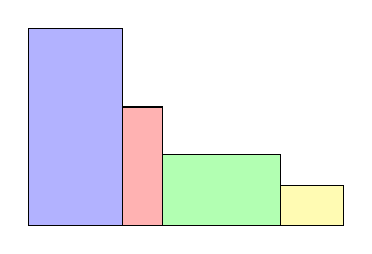
\begin{tikzpicture}
					% 设置矩形的宽度和高度
					\def\rectOneWidth{1.2}
					\def\rectOneHeight{2.5}
					\def\rectTwoWidth{0.5}
					\def\rectTwoHeight{1.5}
					\def\rectThreeWidth{1.5}
					\def\rectThreeHeight{0.9}
					\def\rectFourWidth{0.8}
					\def\rectFourHeight{0.5}
					% 设置矩形之间的间距
					\def\spacing{0}
				
					% 绘制第一个矩形
					\draw[fill=blue!30] (0,0) rectangle ++(\rectOneWidth,\rectOneHeight);
				
					% 绘制第二个矩形
					\draw[fill=red!30] (\rectOneWidth + \spacing,0) rectangle ++(\rectTwoWidth,\rectTwoHeight);
				
					% 绘制第三个矩形
					\draw[fill=green!30] (\rectOneWidth + \rectTwoWidth + \spacing,0) rectangle ++(\rectThreeWidth,\rectThreeHeight);
				
					% 绘制第四个矩形
					\draw[fill=yellow!30] (\rectOneWidth + \rectTwoWidth + \rectThreeWidth + \spacing,0) rectangle ++(\rectFourWidth,\rectFourHeight);
				\end{tikzpicture}
				\qquad
				\longrightarrow
				\qquad
				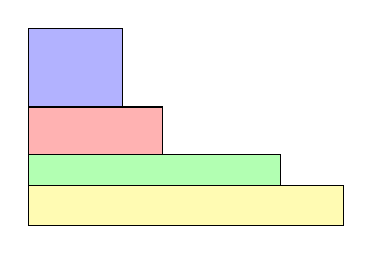
\begin{tikzpicture}
					% 设置矩形的宽度和高度
					\def\rectOneWidth{4}
					\def\rectOneHeight{0.5}
					\def\rectTwoWidth{3.2}
					\def\rectTwoHeight{0.4}
					\def\rectThreeWidth{1.7}
					\def\rectThreeHeight{0.6}
					\def\rectFourWidth{1.2}
					\def\rectFourHeight{1}
					
					% 绘制第一个矩形
					\draw[fill=yellow!30] (0,0) rectangle (\rectOneWidth,\rectOneHeight);
					
					% 绘制第二个矩形
					\draw[fill=green!30] (0,\rectOneHeight) rectangle (\rectTwoWidth,\rectOneHeight+\rectTwoHeight);
					
					% 绘制第三个矩形
					\draw[fill=red!30] (0,\rectOneHeight+\rectTwoHeight) rectangle (\rectThreeWidth,\rectOneHeight+\rectTwoHeight+\rectThreeHeight);
					
					% 绘制第四个矩形
					\draw[fill=blue!30] (0,\rectOneHeight+\rectTwoHeight+\rectThreeHeight) rectangle (\rectFourWidth,\rectOneHeight+\rectTwoHeight+\rectThreeHeight+\rectFourHeight);
				\end{tikzpicture}\]

			\end{thm}
			
			\begin{lma}
			    []
			    {Abel 引理}
			    []
			    []
				若数列 \(\{a_n\}\), \(\{b_n\}\) 满足: 

				(1) \(\{|a_n|\}\) 单调; 

				(2) \(B_n:=\sum\limits_{i=1}^{n}b_i\), \(\{|B_n|\}\) 有上界 \(M\). 

				则: 
				\[\left|\sum_{i=1}^{n}a_i b_i\right|\leq M(|a_1|+2|a_m|)\]
			\end{lma}

			\begin{thm}
			    []
			    {Abel 判别法}
			    []
			    []
				若数列 \(\{a_n\}\), \(\{b_n\}\) 满足: 

				(1) \(\{a_n\}\) 单调有界; 
				
				(2) \(\sum\limits_{n=1}^{+\infty}b_n\) 收敛. 

				则级数 \(\sum\limits_{n=1}^{+\infty}a_n b_n\) 收敛. 
			\end{thm}

			\begin{thm}
			    []
			    {Dirichlet 判别法}
			    []
			    []
				若数列 \(\{a_n\}\), \(\{b_n\}\) 满足: 

				(1) \(\{a_n\}\) 单调收敛于 \(0\); 
				
				(2) \(\sum\limits_{i=1}^{n}b_i\) 有界. 

				则级数 \(\sum\limits_{n=1}^{+\infty}a_n b_n\) 收敛. 
			\end{thm}
			
			\begin{dfn}
			    []
			    {Cauchy 乘积 }
			    [Cauchy Product]
			    []
				设收敛级数 \(\sum\limits_{n=1}^{+\infty}a_n=A\) 与 \(\sum\limits_{n=1}^{+\infty}b_n=B\), 定义二者的 Cauchy 乘积为如下级数: 
				\[\sum_{n=1}^{+\infty}\sum_{k=1}^{n}a_k b_{n+1-k}\]
			\end{dfn}
			
			\begin{thm}
			    []
			    {Mertens 定理 }
			    [Mertens' Theorem]
			    []
				设收敛级数 \(\sum\limits_{n=1}^{+\infty}a_n=A\) 与 \(\sum\limits_{n=1}^{+\infty}b_n=B\), 则: 
				
				两级数中至少有一个绝对收敛 \(\Longrightarrow\) 它们的 Cauchy 乘积收敛. 
			\end{thm}
			
			\begin{thm}
                {}
				若两级数的 Cauchy 乘积收敛, 则其级数和为原来级数和的积. 
			\end{thm}
		
	\section{函数极限}
	
		\subsection{函数极限和Heine定理}
		
			\begin{dfn}
			    []
			    {函数极限}
			    []
			    []
				称函数 \(f\) 在 \(x_0\) 的\textbf{左极限}为 \(a\), 若 \(f\) 在 \(x_0\) 的一个左邻域内有定义,且: 
				\[\forall\varepsilon\in\R^+, \exists\delta\in\R^+(\forall x\in U^-(x_0,\delta), f(x)\in U(a,\varepsilon))\]
				
				记作
				\[\lim_{x\to x_0-}f(x)=a\]
				
				称函数 \(f\) 在 \(x_0\) 的\textbf{右极限}为 \(b\), 若 \(f\) 在 \(x_0\) 的一个右邻域内有定义,且: 
				\[\forall\varepsilon\in\R^+, \exists\delta\in\R^+(\forall x\in U^+(x_0,\delta), f(x)\in U(b,\varepsilon))\]
				
				记作
				\[\lim_{x\to x_0+}f(x)=b\]
				
				称函数 \(f\) 在 \(x_0\) 的\textbf{极限}为 \(c\), 若: 
				\[\forall\varepsilon\in\R^+, \exists\delta\in\R^+(\forall x\in\U(x_0,\delta), f(x)\in U(c,\varepsilon))\]
				
				记作
				\[\lim_{x\to x_0}f(x)=c\]

				函数极限的等价定义: 
				\[\lim_{x\to x_0}f(x):=\lim_{x\to x_0-}f(x)=\lim_{x\to x_0+}f(x)=c\]
			\end{dfn}
			
			\begin{thm}
			    []
			    {Heine定理}
			    []
			    []
				内容: 
				\[\lim_{x\to x_0}f(x)=a\iff\forall\{x_n\}: \lim_{n\to+\infty} x_n=x_0, \lim_{n\to+\infty} f(x_n)=a\]
			\end{thm}

                \begin{prf}
			证明: 
			
				(1)\[\lim_{x\to x_0}f(x)=a\iff \forall\varepsilon_1\in\R^+, \exists\delta\in\R^+(\forall x\in\U(x_0,\delta), f(x)\in o(a,\varepsilon_1))\]
				\[\lim_{n\to+\infty} x_n=x_0\iff\forall\varepsilon_2\in\R^+,\exists N_2\in\mathbb{Z}^+(\forall n>N_2, x_n\in o(x_0,\varepsilon_2))\]
				\[\lim_{n\to+\infty} f(x_n)=a\iff\forall\varepsilon_3\in\R^+,\exists N_3\in\mathbb{Z}^+(\forall n>N_3, f(x_n)\in o(a,\varepsilon_3))\]
				
				(2)充分性: 
				
				\[\lim_{x\to x_0}f(x)=a\]
				\[\varepsilon_1:=\varepsilon_3, \varepsilon_2:=\delta\]
				\[\exists N=max\{N_1,N_2\}(\forall n>N, x_n\in\U(x_0,\delta)\Longrightarrow f(x_n)\in U(a,\varepsilon_3))\]
				\[\Longrightarrow\lim_{n\to+\infty}f(x_n)=a\]
				
				(3)必要性: 运用反证法. 假设: 
				\[\lim_{x\to x_0}f(x)\neq a; \forall\{x_n\}: \lim_{n\to+\infty} x_n=x_0,\lim_{n\to+\infty} f(x_n)=a\]
				\[\lim_{x\to x_0}f(x)\neq a\iff\exists\varepsilon_1\in\R^+: \forall \delta\in\R^+, \exists x\in\U(x_0,\delta): f(x)\notin U(a,\varepsilon_1)\]
				
				不妨设 \(f\) 在 \(\U(x_0,\delta_0)\) 内有定义, 
				\[\delta_i:=\frac{\delta_0}{i}\Longrightarrow\forall i\in\N^*, \exists x_i\in \U(x_0,\delta_0)(f(x)\notin o(a,\varepsilon_1))\]
				
				如此取得无穷数列 \(\{x_n\}\) : 
				\[\forall\varepsilon_2\in\R^+, N:=\left[\frac{1}{\varepsilon_2}\right]+1, \forall n>N, |x_n-x_0|<\frac{1}{\left[\dfrac{1}{\varepsilon_2}\right]+1}<\varepsilon_2\Longrightarrow\lim_{n\to+\infty}x_n=x_0\]
				
				又 \(\lim\limits_{n\to+\infty}f(x_n)\neq a\), 与 \(\forall\{x_n\}: \lim\limits_{n\to+\infty} x_n=x_0,\lim\limits_{n\to+\infty} f(x_n)=a\) 矛盾. \(\square\)
				\end{prf}
                由Henie定理, 可以立得等价于数列极限性质的函数极限性质: 
    
			\begin{ppt}
			    []
			    {函数极限的唯一性}
			    []
			    []
				若 \(\lim\limits_{x\to\x_0}f(x)\) 存在, 则它是唯一的.
			\end{ppt}

			\begin{ppt}
			    []
			    {函数极限的局部有界性}
			    []
			    []
				函数 \(f:D\to\R\) 在 \(x_0\) 处极限存在 \(\Longrightarrow\exists U(x_0)\subseteq D: f\) 在 \(U(x_0)\) 上有界. 
				
			
			\end{ppt}

			

			\begin{ppt}
			    []
			    {夹逼定理 (迫敛性) }
			    []
			    []
				设函数 \(f,g\) 与 \(h\) 在 \(x_0\) 的一个邻域内满足
				\[f(x)\leq h(x)\leq g(x).\]
				则\[\lim\limits_{x\to\x_0}f(x)=\lim\limits_{x\to\x_0}g(x)=l\Longrightarrow\lim\limits_{x\to\x_0}h(x)=l.\]
			\end{ppt}

			\begin{ppt}
			    []
			    {函数极限的保序性}
			    []
			    []
				函数 \(f,g\) 在 \(x_0\) 的一个去心邻域内满足 \(f(x)\leq g(x)\), \(x_0\) 处极限存在, 则
					\[\lim\limits_{x\to\x_0}f(x)\leq\lim\limits_{x\to\x_0}g(x).\]
			\end{ppt}
   
			\begin{prf}
				证: 设 \(\displaystyle\lim_{x\rightarrow x_0}f(x)=A , \displaystyle\lim_{x\rightarrow x_0}g(x)=B\) , 则对 \(\forall\varepsilon>0\) , 分别\(\exists \ \delta_1 , \delta_2 >0 \ s.t.\) \\
				当 \(0<|x-x_0|<\delta_1\) 时有 \(A-\varepsilon<f(x),\)当 \(0<|x-x_0|<\delta_2\) 时有 \(g(x)<B+\varepsilon.\)\\
				因此, 令 \(\delta=\min\{\delta^\prime,\delta_1,\delta_2\}\) , 则当 
				\(0<|x-x_0|<\delta\) 时, 不等式 
				\(f(x)\leq g(x)\) 与上两式同时成立, \\
				于是有 \(A-\varepsilon<f(x)\leq g(x)<B+\varepsilon,\)\\
				从而 
				\(A<B+2\varepsilon\) . 再根据 
				\(\varepsilon\) 的任意性可以推出 \(A\leq B\) , 证毕.  \(\square\)
			\end{prf}
   
            \begin{ppt}
			    []
			    {函数极限的保号性}
			    []
			    []
                内容: 
                \[f:D\to\R,\displaystyle\lim_{x\rightarrow x_0}f(x)=A>0\Longrightarrow\forall 0<r<A,\exists \U(x_0)\ s.t. \forall x\in \U(x_0),f(x)>r>0.\]
            \end{ppt}

				\begin{prf}
				设 \(A > 0\), 对任意 \(r \in (0, A)\), 取 \(\varepsilon = A - r\), 则根据函数极限定义, 存在 \(\delta > 0\), 使得对一切 \(x \in \U(x_0, \delta)\) 有\[r = A - \varepsilon < f(x),\]
			    故证毕, 对于 \(A < 0\) 的情形可以类似地证明. \(\Box\)
				\end{prf}
   
            \begin{ppt}
			    []
			    {}
			    []
			    []
				有限常数极限关于四则运算不变: 
				\[\lim_{x\to\x_0}f(x)=A, \lim_{x\to\x_0}g(x)=B\Longrightarrow
				\begin{cases}
					\lim\limits_{x\to\x_0}\left(f(x)\pm g(x)\right) & =A\pm B\\
					\lim\limits_{x\to\x_0}(f(x)\cdot g(x)) & =A\cdot B\\
					\lim\limits_{x\to\x_0}\left(\dfrac{f(x)}{g(x)}\right) & =\dfrac{A}{B} \ (B\neq 0)\\
				\end{cases}\]
			\end{ppt}
                
			当然, 我们也可以得到函数极限形式的Cauchy收敛定理: 
       
            \begin{thm}
			    []
			    {Cauchy收敛定理}
			    []
			    []
				函数 \(f\) 在 \(x_0\) 处极限存在\(\Longleftrightarrow\forall\varepsilon >0,\exists \delta >0\ s.t,\forall x_1,x_2\in\U(x_0,\delta),|f(x_1)-f(x_0)|<\varepsilon.\)
			\end{thm}

   			\begin{xmp}
			    []
			    {Riemann 函数}
			    []
			    []
				内容: 
				\[ R(x) = 
                \begin{cases} 
                1, & x = 0 \\
                \frac{1}{q}, & x = \frac{p}{q}, \, p, q \in \mathbb{N}^*, \, (p, q) = 1 \\
                0, & x \in \mathbb{R} \setminus \mathbb{Q}
                \end{cases}
                \] 

                则\(\forall x_0 \in \mathbb{R}, \lim\limits_{x \to x_0} R(x) = 0.\) 
            \end{xmp}

                \begin{prf}
                 \( R(x+1) = R(x) \),  \(\therefore\)  只需证  \( x \in [0,1] \)  的情况; 又只需证  \( x_0 \)  为有理数. 

                 \(\because \forall \varepsilon > 0\) , 取  \( q_0 > \frac{1}{\varepsilon} \) , 则  \( (x_0 - 1, x_0 + 1) \)  上分母小于  \( q_0 \)  的数只有有限个, 

                记其中离  \( x_0 \)  最近的为  \( x_N \) , 取  \( 0 < \delta < |x_N - x_0| \) , 则  \( 0 < |x - x_0| < \delta \)  时, 

                 \( |R(x) - 0| < \frac{1}{q_0} < \varepsilon \) ,  \(\therefore \lim\limits_{x \to x_0} R(x) = 0. \ \square\) 
                \end{prf}

        	\begin{thm}
			    []
			    {复合函数的极限}
			    []
			    []
				设 \(\lim\limits_{x \to x_0} f(x) = l\), \(\lim\limits_{t \to t_0} g(t) = x_0\). 如果在 \(t_0\) 的某个邻域 \(\U(t_0)\) 内 \(g(t) \neq x_0\), 则

				 \[
				\lim\limits_{t \to t_0} f(g(t)) = l.
				\] 
			\end{thm}
   
		\subsection{函数的连续性}
			
			\begin{dfn}
			    []
			    {连续}
			    [Continuous]
			    []
				称 \(f\) 在 \(x_0\) 点是\textbf{连续(Continuous)}的, 若 \(f\) 在 \(x_0\) 的一个邻域内有定义, 且: 
				\[\lim_{x\to x_0-}f(x)=\lim_{x\to x_0+}f(x)=f(x_0)\]
				
				称 \(f\) 在 \(x_0\) 点\textbf{左连续}, 若 \(f\) 在 \(x_0\) 的一个左邻域内有定义, 且: 
				\[\lim_{x\to x_0-}f(x)=f(x_0)\]
				
				称 \(f\) 在 \(x_0\) 点\textbf{右连续}, 若 \(f\) 在 \(x_0\) 的一个右邻域内有定义, 且: 
				\[\lim_{x\to x_0+}f(x)=f(x_0)\]
			\end{dfn}

			\begin{ppt}
			    []
			    {连续函数的局部有界性}
			    []
			    []
				\(f:D\to\R\)在 \(x_0\in D\) 处连续 \(\Longrightarrow\exists U(x_0)\subseteq D: f\) 在 \(U(x_0)\) 上有界. 
			\end{ppt}

			\begin{ppt}
			    []
			    {函数的四则运算保持连续性}
			    []
			    []
				\(f_1:D_1\to\R,f_2:D_2\to\R\)在 \(x_0\in D_1\cap D_2\) 处连续 \(\Longrightarrow\) 在 \(x_0\) 处有: 
				\(f_1+f_2,f_1\cdot f_2,\dfrac{f_1}{f_2}(f_2(x_0)\neq 0)\)均在 \(x_0\) 处连续. 
			\end{ppt}
			
			\begin{ppt}
			    []
			    {函数的复合保持连续性}
			    []
			    []
				\(f:X\to Y,g:Y\to\R(X,Y\subseteq\R)\), 设 \(f(a)=b\), \(f\)在 \(a\) 处连续, \(g\)在 \(b\) 处连续, 则 \(g\circ f\) 在 \(a\) 处连续. 
			\end{ppt}
			
			\begin{dfn}
			    []
			    {不连续点}
			    [Discontinuity]
			    []
				称 \(x_0\) 是 \(f\) 的一个\textbf{第一类间断点/不连续点}, 若: 
				\[\exists\lim_{x\to x_0-}f(x), \lim_{x\to x_0+}f(x)\]
				
				称 \(x_0\) 是 \(f\) 的一个\textbf{第二类间断点/不连续点}, 若
				\[\nexists\lim_{x\to x_0-}f(x)\vee\nexists\lim_{x\to x_0+}f(x)\]
				
				其中称 \(x_0\) 是 \(f\) 的一个\textbf{可去间断点/不连续点(Removable Discontinuity)}, 若: 
				\[\lim_{x\to x_0-}f(x)=\lim_{x\to x_0+}f(x)=a\]
				
				但 \(f(x_0)\) 无定义或 \(f(x_0)\neq a\). 
				
				称 \(x_0\) 是 \(f\) 的一个\textbf{跳跃间断点/不连续点(Jump Discontinuity)}, 若
				\[\lim_{x\to x_0-}f(x)\neq\lim_{x\to x_0+}f(x)\]
			\end{dfn}
			
			\begin{dfn}
			    []
			    {连续函数}
			    [Continuous Function]
			    []
				函数 \(f:D\to\R\) 称为在开区间 \((a,b)\subseteq D\) 上\textbf{连续}, 若 \(\forall x\in(a,b)\), \(f\)在 \(x\) 处连续. 

				\(f\)称为在 \([a,b]\subseteq D\) 上连续, 若 \(f\) 在 \((a,b)\) 上\textbf{连续}, 在 \(a\) 处右连续, 在 \(b\) 处左连续. 
			\end{dfn}

   			\begin{ppt}
			    []
			    {反函数的连续性}
			    []
			    []
				If \(y, f(x) \in C[a, b]\) and \(f(x)\) 严格递增, \(f(a) = \alpha\), \(f(b) = \beta\).

                则 \(x = f^{-1}(y)\ \exists\) 且 \(f^{-1}(y) \in C\left[\alpha, \beta\right]\).
			\end{ppt}

			\begin{prf}
			先证 \(\left\{f(x) \mid x \in [a, b]\right\} = \left[\alpha, \beta\right] \Leftrightarrow \forall y \in (\alpha, \beta), \exists x \in (a, b), f(x_0) = y\),


                 \[x_0 := \sup\{x \in [a, b] \mid f(x) < y\} := \sup S,\] 
                 \[
                \lim\limits_{\delta \to 0} f(a + \delta) = f(a) < y \Rightarrow \text{If}  0 << \delta < 1, f(a + \delta) < y.
                \] 

                又 \(f\) 严格递增 \(\Rightarrow x \in\cointerval{a}{a+\delta}\) 时,  \(f(x) < f(a+\delta) < y\) ,  \(\therefore x_0 \geq a + \delta\) , 

                 \(
                \therefore x_0 > a, \text{同理 }\  x_0 < b, \therefore x_0 \in (a, b), \ \text{此时 }\  \forall x \in (a, x_0), f(x) < y,
                \)

                \(\forall x \in (x_0, b)\),  \(f(x) > y \Rightarrow \lim\limits_{x \to x_0^-} f(x) \leq y \leq \lim\limits_{x \to x_0^+} f(x)\) , 又 \(\lim\limits_{x \to x_0} f(x) = f(x_0)\), 

                \[
                \therefore f(x_0) = y. \quad \square
                \] 

                下证 \(f^{-1}(y) \in C[\alpha, \beta] \Leftrightarrow \forall y_0 \in [\alpha, \beta], \forall \varepsilon > 0, \exists \delta > 0 \text{ s.t. } 0 < |y - y_0| < \delta \text{ 时},\)


                 \[
                |f^{-1}(y) - f^{-1}(y_0)| < \varepsilon. \] 

                \(\text{记 }\  x_0 = f^{-1}(y_0), x = f^{-1}(y), y \in (\alpha, \beta),
                \)



                \(\text{取 }\  0 < \varepsilon << 1, y_0 - \varepsilon, y_0 + \varepsilon \in (\alpha, \beta), \text{记 }\  \delta_1 = y_0 - f(x_0 - \varepsilon) > 0, \delta_2 = f(x_0 + \varepsilon) - y_0 > 0,\)



 
                \(\text{取 }\  \delta = \min\{\delta_1, \delta_2\}, \text{当 }\  |y - y_0| < \delta \text{ 时},\)
                \[f(x_0 - \varepsilon) = y_0 - \delta_1 \leq y_0 - \delta < y < y_0 + \delta \leq y_0 + \delta_1 = f(x_0 + \varepsilon),\]
                 \(
                \text{又 }\  x = f^{-1}(y) \text{严格递增},\  \therefore x_0 - \xi < f^{-1}(y) < x_0 + \xi, \text{即}\  |f^{-1}(y) - x_0| < \xi. \quad \square
                \) 
			\end{prf}

			\begin{thm}
			    []
			    {Bolzano-Cauchy介值定理}
			    []
			    []
				设函数 \(f:[a,b]\to\R(a<b)\) 在 \([a,b]\) 上连续, 且 \(f(a)\cdot f(b)<0\Longrightarrow\exists x_0\in(a,b)(f(x_0)=0)\). 
			\end{thm}

			\begin{prf}
			
				运用反证法. 假设 \(\forall x\in(a,b), f(x)\neq 0\), 则可如下归纳构造闭区间族 \(\mathcal{D}\) : 
				\[\mathcal{D}:=\{D_{i,j}|D_{i,j}=[\frac{1}{2^i}(ja+(2^i-j)b),\frac{1}{2^i}((2^i-j)a+jb)],i,j\in\N,1\leq j\leq 2^i\}\]

				可作如下断言: 
				\[\exists x_1,x_2\in D_{i,j}(f(x_1)f(x_2)<0)\Longrightarrow\exists x'_1,x'_2\in D_{i+1,j'}\subseteq D_{i,j}(f(x'_1)f(x'_2)<0)\]
				
				这是因为只有 \(D_{i+1,2j-1}\) 和 \(D_{i+1,2j}\) 符合条件, 有: 
				\[D_{i+1,2j-1}\cup D_{i+1,2j}=D_{i,j}\wedge D_{i+1,2j-1}\cap D_{i+1,2j}=\{x_{i,j}\}\]
				\[x_{i,j}\neq 0\Longrightarrow x_{i,j}>0\vee x_{i,j}<0\]
				
				这意味着假若断言不正确, 则 \(f(D_{i+1,2j-1})\) 和 \(f(D_{i+1,2j})\) 内所有元素均必须与 \(x_{i,j}\) 同号, 与断言条件矛盾, 故断言正确. 

				选择符合条件的 \(D_{i+1,j'}\), 记作 \(D_{i+1}\). 记 \(D_0=D_{0,1}\), 令 \(i\) 遍历 \(\N\), 得到闭区间序列\(\mathcal{D}'=\{D_i|i\in\N\}\)

				容易验证 \(\mathcal{D}'\) 是区间长度收敛于 \(0\) 的闭区间套, 由Cauchy-Cantor闭区间套定理, 有: 
				\[\bigcap_{i\in\N}\mathcal{D}'=\{x_0\}\subseteq[a,b]\]

				不妨设 \(f(x_0)>0\), 则: 
				\[\forall D_i\in\mathcal{D}', \exists\xi_i\in D_i(f(\xi_i)<0)\Longrightarrow\lim_{n\to+\infty}\xi_n=x_0\]

				由Heine定理, \(\lim\limits_{n\to+\infty}f(\xi_n)=f(\lim\limits_{n\to+\infty}\xi_n)=f(x_0)>0\), 与 \(f(\xi_i)<0\) 矛盾. \(\square\)
                \end{prf}
			
			\begin{thm}
			    []
			    {Weiestrass最值定理}
			    []
			    []
				定义在闭区间上的连续函数 \(f:[a,b]\to\R\) 在 \([a,b]\) 上有界, 且值域有最值: \[\exists x_M\in[a,b](f(x_M)=f_{\max}([a,b])),\exists x_m\in[a,b](f(x_m)=f_{\min}([a,b]))\]
			\end{thm}

			\begin{prf}

				运用反证法. 不妨假设 \(f\) 无上界, 即 \(\forall M\in\R^+, \exists x\in[a,b]:f(x)>M\). 

				令 \(M\) 遍历 \(\N\), 得到数列 \(\{x_n\}(\forall n\in\N, f(x_n)>n)\). 
				
				即有\(\lim\limits_{n\to+\infty}f(x_n)=+\infty\)

				由Bolzano-Weiestrass定理, 可以选出 \(\{x_n\}\) 的一个收敛子列 \(\{x_n'\}\). 
				
				设 \(\lim\limits_{n\to+\infty}=x_0\), \(f\)连续, 可由Heine定理得\(\lim\limits_{n\to+\infty}f(x_n)=f(\lim\limits_{n\to+\infty}x_n)=f(x_0)\)

				于是 \(f(x_0)=+\infty\), 无意义, 矛盾. 
				
				即 \(f\) 在 \([a,b]\) 上有上界, 同理可证其有下界. 

				下运用连续函数的拓扑性质证明确界在值域内: 

				\(f\)是连续的, \([a,b]\)是闭的 \(\Longrightarrow f([a,b])\) 是闭的. 

				又 \(f([a,b])\) 有界, \(\exists\sup f([a,b]),\inf f([a,b])\). 
				\[\forall U(\sup f([a,b])), \exists x_1\in[a,b](f(x_1)\in U(\sup f([a,b])))\]
				\[\forall U(\inf f([a,b])), \exists x_2\in[a,b](f(x_2)\in U(\inf f([a,b])))\]
				
				由Bolzano-Cauchy介值定理知: 
				\[\forall C\in[f(x_1),f(x_2)], \exists x\in[a,b]: f(x)=C\]
				\[\Longrightarrow\forall C\in(\inf f([a,b]),\sup f([a,b])), \exists x\in[a,b]: f(x)=C\]
				\[\Longrightarrow (\inf f([a,b]),\sup f([a,b]))\subseteq f([a,b])\]
				\[f([a,b])\cap((-\infty,\inf f([a,b]))\cup(\sup f([a,b]),+\infty))=\varnothing\]

				于是 \(f([a,b])\) 只能是以 \(\inf f([a,b]),\sup f([a,b])\) 为端点的区间. 

				而这其中, 只有 \([\inf f([a,b]),\sup f([a,b])]\) 是闭的. 
				\[\Longrightarrow f([a,b])=[\inf f([a,b]),\sup f([a,b])]\square\]
                \end{prf}
			
		\subsection{函数的一致连续性}
			
			\begin{dfn}
			    []
			    {}
			    []
			    []
				称 \(f\) 在区间 \(D\) 上\textbf{一致连续(Uniformly Continuous)}, 若: 
				\[\forall\varepsilon\in\R^+, \exists\delta\in\R^+: \forall x_1,x_2\in D: |x_1-x_2|<\delta, |f(x_1)-f(x_2)|<\varepsilon\]
			\end{dfn}
			
			\begin{thm}
			    []
			    {Cantor-Heine 一致连续性定理}
			    []
			    []
				定义在闭区间上的连续函数一致连续. 
			\end{thm}

    		\begin{prf}
				 (反证法) 若 \(f\) 在 \([a,b]\) 不一致连续, 即
				\[\exists\varepsilon_0>0,s_n,t_n\in[a,b],|s_n-t_n|\to 0\ s.t.|f(s_n)-f(t_n)|\geq\varepsilon_0\tag{1}\]\ 
				由列紧性,  \(\exists s_{k_n}\to s\in[a,b]\),
				此时 \(|t_{k_n}-s_{k_n}|+|s_{k_n}-s|\to 0\),\ \(\therefore t_{k_n}\to s\).
				\[\Longrightarrow\lim_{n\to\infty}f(s_{k_n})=\lim_{n\to\infty}f(t_{k_n})=f(s) \\
				\Longrightarrow\lim_{n\to\infty}|f(s_{k_n})-f(t_{k_n})|=0,\]
				与(1)矛盾. \(\square\)
			\end{prf}
				


		
	
	\section{一元微分和导数}
		
		\subsection{一元微分和导数}
		
			\begin{dfn}
			    []
			    {}
			    []
			    []
				设函数 \(f:D\to\R(D\subseteq\R)\) 在 \(x_0\in D\) 处连续, 且在 \(x_0\) 的一个邻域 \(\U(x_0,\delta)\) 内有定义. 记 \(y=f(x)\), 称函数 \(f\) 在 \(x_0\) 处\textbf{可微(Differentiable)}或\textbf{可导}, 若: 
				\[\exists k\in\R(\exists\delta_0\in\R^+(x\in\U(x_0,\delta_0)\Longrightarrow y-y_0=k(x-x_0)+o(x-x_0)))\]
				
				记 \(\Delta y=y-y_0,\Delta x=x-x_0\), 上式写作: 
				\[\Delta y=k\Delta x+o(\Delta x)\]
				
				称该式的线性主部确定了 \(y\) 在 \(x_0\) 处的一个\textbf{微分(Differential)}, 记为
				\[\dd y=k\dd x\]
				
				其中常数 \(k\) 称为 \(f\) 在 \(x_0\) 处的\textbf{导数(Derivative)}或\textbf{微商}, 记为
				\[f'(x_0)=k=\frac{\dd y}{\dd x}\]
			\end{dfn}
			
			\begin{ppt}
			    []
			    {}
			    []
			    []
				内容: 
				\[\mbox{函数 \(f\) 在 \(x_0\) 处可微}\iff\exists\lim_{\Delta x\to 0}\frac{f(x_0+\Delta x)-f(x_0)}{\Delta x}\]
				\[f'(x_0)=\lim_{\Delta x\to 0}\frac{f(x_0+\Delta x)-f(x_0)}{\Delta x}\]
			\end{ppt}
			
			\begin{ppt}
			    []
			    {}
			    []
			    []
				函数 \(f:D\to\R\) 在 \(x_0\in\R\) 处可微 \(\Longrightarrow f\) 在 \(x_0\) 处连续. 
			\end{ppt}

            \begin{prf} 

				\(f:D\to\R\)在 \(x_0\in\R\) 处可微\(\iff\exists k\in\R(\exists\delta_0\in\R^+(\forall|\Delta x|<\delta_0\Longrightarrow\Delta y=k\Delta x+o(\Delta x)))\)
				\[\iff\forall\varepsilon_1\in\R^+,\exists\delta_1\in\R^+(\forall|\Delta x|<\delta_1\Longrightarrow\Delta y-k\Delta x<\varepsilon_1\Delta x)\]
				
				\(f\)在 \(x_0\) 处连续\(\iff\forall\varepsilon_2\in\R^+,\exists\delta_2\in\R^+(\forall|\Delta x|<\delta_2\Longrightarrow|\Delta y|<\varepsilon_2)\)
				\[|\Delta y|<|(k+\varepsilon_1)\Delta x|\leq(|k|+\varepsilon_1)|\Delta x|(|\Delta x|<\delta_1)\]

				只需确保 \(|\Delta x|<\dfrac{\varepsilon_2}{|k|+\varepsilon_1}\), 即令\(\delta_2:=\min\left\{\delta_1,\dfrac{\varepsilon_2}{|k|+\varepsilon_1}\right\}\Longrightarrow|\Delta y|<\varepsilon_2\square\)
            \end{prf}
			
			\begin{dfn}
			    []
			    {}
			    []
			    []
				称函数 \(f:D\to\R(D\subseteq\R)\) 在 \(D'\subseteq D\) 上\textbf{可微(Differentiable)}或\textbf{可导}, 若 \(\forall x_0\in D'\), \(f\)在 \(x_0\) 处可微. 
				
				\(f':D'\to\R\)是一个以 \(x_0\) 为自变量的函数, 称为 \(f\) 在 \(D'\) 上的\textbf{导函数(Derivative Function)}. 
			\end{dfn}
				
			\begin{ppt}
			    []
			    {}
			    []
			    []
				设 \(f,g\) 在 \(D\) 上可导, 则: 
				\[(f+g)'(x)=f'(x)+g'(x)\]
			\end{ppt}
			
			\begin{ppt}
			    []
			    {}
			    []
			    []
				设 \(f\) 在 \(D\) 上可导, 则: 
				\[\forall k\in\R, (kf)'(x)=kf'(x)\]
			\end{ppt}
			
			\begin{ppt}
			    []
			    {}
			    []
			    []
				设 \(f,g\) 在 \(D\) 上可导, 则: 
				\[(f\cdot g)'(x)=f'(x)g(x)+f(x)g'(x)\]
			\end{ppt}
			
			\begin{ppt}
			    []
			    {}
			    []
			    []
				设 \(f,g\) 在 \(D\) 上可导, 则: 
				\[(\frac{f(x)}{g(x)})'=\frac{f'(x)g(x)-f(x)g'(x)}{g^2(x)}\]
			\end{ppt}
			
			\begin{ppt}
			    []
			    {}
			    []
			    []
				一阶微分的形式不变性: 
				
				设 \(y\) 是关于 \(u\) 的函数, \(u\)是关于 \(x\) 的函数, \(u=u_0|_{x=x_0}\); 
				
				设 \(y\) 在 \(u_0\) 处可微且 \(\dd y=k\dd u|_{u=u_0}\), \(u\)在 \(x_0\) 处可微且 \(\dd u=l\dd x|_{x=x_0}\), 则: 
				\[\dd y=kl\dd x|_{x=x_0}\]
			\end{ppt}

            \begin{prf} 
				\[\dd y=k\dd u|_{u=u_0}\iff\Delta y=k\Delta u+o(\Delta u)\]
				\[\dd u=l\dd x|_{x=x_0}\iff\Delta u=l\Delta x+o(\Delta x)\]
				\[\begin{array}{rcl}\Longrightarrow\Delta y & = & k[l\Delta x+o(\Delta x)]+o(\Delta u)\\
				 & = & kl\Delta x+ko(\Delta x)+o(k\Delta x+o(\Delta x))\\
				 & = & kl\Delta x+o(\Delta x)
				 \end{array}\]
				
				即\[\dd y=kl\dd x|_{x=x_0}\square\]
			\end{prf}
				
			
			\begin{ppt}
				{复合函数求导链式法则}
				\[(f\circ g)'(x)=[f'\circ g(x)]\cdot g'(x)\]
			\end{ppt}
			
            \begin{prf} 			
				由一阶微分形式不变性可立即得到. \(\square\)
			\end{prf}
    
			\begin{ppt}
			    []
			    {}
			    []
			    []
				反函数求导法则: 

                设  \( y = f(x) \)  在包含  \( x_0 \)  的区间  \( I \)  上连续且严格单调, 若它在  \( x_0 \)  处可导, 且  \( f'(x_0) \neq 0 \) , 那么它的反函数  \( x = f^{-1}(y) \)  在  \( y_0 = f(x_0) \)  处可导, 且
                \[\left( f^{-1} \right)'(y_0) = \frac{1}{f'(x_0)}\]
			\end{ppt}
			
			\begin{ppt}
			    []
			    {}
			    []
			    []
				奇函数的导函数是偶函数, 偶函数的导函数是奇函数. 
			\end{ppt}
				
				
			
		\subsection{七类基本初等函数的导数}
			
			在基本初等函数的定义域内, 有: 
			
			\begin{xmp}
			    []
			    {}
			    []
			    []
				常数函数导数: 
				\[C'=0\]
			\end{xmp}
			
			\begin{xmp}
			    []
			    {}
			    []
			    []
				幂函数导数: 
				\[(x^a)'=ax^{a-1}(a\neq 0)\]
			\end{xmp}
			
			\begin{xmp}
			    []
			    {}
			    []
			    []
				指数函数导数: 
				\[(a^x)'=(\ln a)x^a(a\in\R^+-\{1\})\]
				
				特别地, \[(e^x)'=e^x\]
			\end{xmp}
			
			\begin{xmp}
			    []
			    {}
			    []
			    []
				对数函数导数: 
				\[(\log_ax)'=\frac{1}{(\ln a)x}\]
				
				特别地, 
				\[(\ln x)'=\frac{1}{x}\]
			\end{xmp}
			
			\begin{xmp}
			    []
			    {}
			    []
			    []
				三角函数导数: 
				\[\begin{array}{ccc}
				\sin'x=\cos x & \cos'x=-\sin x & \tan'x=\sec^2x\\
				\csc'x=-\csc x\cot x & \sec'x=\tan x\sec x & \cot'x=-\csc^2x
				\end{array}\]
			\end{xmp}
			
			\begin{xmp}
			    []
			    {}
			    []
			    []
				反三角函数导数: \[\begin{array}{ccc}
				\arcsin'x=\dfrac{1}{\sqrt{1-x^2}} & \arccos'x=-\dfrac{1}{\sqrt{1-x^2}} & \arctan'x=\dfrac{1}{1+x^2}\\
				\arccsc'x=-\dfrac{1}{|x|\sqrt{x^2-1}} & \arcsec'x=-\dfrac{1}{|x|\sqrt{x^2-1}} & \arccot'x=-\dfrac{1}{1+x^2}
				\end{array}\]
			\end{xmp}
			
			\begin{xmp}
			    []
			    {}
			    []
			    []
			 	双曲函数导数: 
				\[\begin{array}{ccc}
			 	\sinh 'x=\cosh x & \cosh'x=\sinh x & \tanh'x=
			 	\end{array}\]
			\end{xmp}
		
        \subsection{高阶微分/导数}
			
			\begin{dfn}
			    []
			    {高阶微分/导数}
			    []
			    []
				设函数 \(y=f(x)\) 在 \(x_0\) 可微, 将 \(\dd y=k_1\dd x|_{x=x_0}\) 视为 \(y\) 的一阶微分; 
				
				设 \(\dd^{n-1}y=k_{n-1}\dd x^{n-1}|_{x=x_0}\) 是 \(y\) 在 \(x_0\) 处的 \(n-1\) 阶微分 \((n\in\mathbb{Z}^+-\{1\})\), 
				
				若
				\[\exists k_n\in\R(\dd^ny:=\dd(\dd^{n-1} y)=\dd(k_{n-1}\dd x^{n-1})=k_n\dd x^n|_{x=x_0})\]
				
				称 \(y\) 在 \(x_0\) 处 \(n\) 阶可微/可导, 并称上式为 \(y\) 在 \(x_0\) 处的\textbf{ \(n\) 阶微分}; 
				
				称 \(k_n=\dfrac{\dd^ny}{\dd x^n}(x_0)\) 为 \(y\) 在 \(x_0\) 处的\textbf{ \(n\) 阶导数}. 
				
				\(k_n\)是一个关于 \(x_0\) 的函数, 称为 \(y\) 的\textbf{ \(n\) 阶导函数}, 可归纳地记为\(f^{(n)}:=(f^{(n-1)})'\)
			\end{dfn}

            \begin{thm}
			    []
			    {Leibniz公式}
			    []
			    []
				函数 \(u\) 、 \(v\) 、 \(uv\) 在区间 \(I\) 上 \(n\) 阶可导, 则
				\[(uv)^{(n)} = \sum_{k=0}^{n} C_{n}^{k} u^{(n-k)} v^{(k)}.\]
			\end{thm}
			
			\begin{prf}
				 (自然语言) 这里我们不使用归纳法证明, 而是探讨其组合意义及与二项式定理的关系: 

				我们知道,  \(u^{(1)} v\) 可以由 \(uv\) 求一次导得到, 而 \(u^{(2)} v\) 可以由 \(u^{(1)} v\) 再求一次导得到; 

				我们记 \(u^{(2)} v\) 得到的过程为 \(u \cdot u\)  (或2个“ \(u\) 变换”) ;

				一般地, 任意的 \(u^{(n-k)} v^{(k)}\) 可以由 \((n-k)\) 个“ \(u\) 变换”和 \(k\) 个“ \(v\) 变换”的过程得到, 可以记作类似“ \(u\cdot v \cdot u \cdot \dots \cdot v\) ”的形式; 

				不难发现, 这样得到的过程序列中 \(u\) 、 \(v\) 的顺序可以任意交换, 所有不同顺序的过程存在且唯一, 
				因此, 由组合数的定义知,  \(u^{(n-k)} v^{(k)}\) 的系数为 \(C_{n}^{k}\).\(\square\)
			\end{prf}

			
		\subsection{函数凸性与Jenson不等式}
			\begin{dfn}
			    []
			    {}
			    []
			    []
				设函数 \(f\) 在区间 \(I\) 上有定义,如果 \(\forall \ x_1, x_2 \in I, x_1 \neq x_2\) , 以及 \( \forall \ \lambda_1, \lambda_2 > 0\) , 且 \(\lambda_1 + \lambda_2 = 1\), 都有
				\[
				f(\lambda_1 x_1 + \lambda_2 x_2) \leq \lambda_1 f(x_1) + \lambda_2 f(x_2),
				\]
				则称 \(f\) 为 \(I\) 上的\textbf{凸函数}. 如果上述不等式对 \(\forall \  x_1 \neq x_2\) 及 \(\lambda_1, \lambda_2 > 0 \ (\lambda_1 + \lambda_2 = 1)\) 不等号总成立, 则称 \(f\) 为 \(I\) 上的\textbf{严格凸函数}.					
			\end{dfn}
			
			\begin{thm}
			    []
			    {Jenson不等式}
			    []
			    []
				设 \(f\) 在区间 \(I\) 上是凸函数, 则对任何 \(x_1, x_2, \cdots, x_n \in I\), 以及 \(\lambda_1, \lambda_2, \cdots, \lambda_n > 0\), 且 \(\lambda_1 + \lambda_2 + \cdots + \lambda_n = 1\), 都有
				\[f\left(\sum_{i=1}^n \lambda_i x_i\right) \leq \sum_{i=1}^n \lambda_i f(x_i). \]

				若 \(f\) 是 \(I\) 上的严格凸函数, 则当 \(x_1, x_2, \cdots, x_n\) 不全相等时, 有
				\[f\left(\sum_{i=1}^n \lambda_i x_i\right) < \sum_{i=1}^n \lambda_i f(x_i). \]
			\end{thm}

			\begin{prf}
				 (数学归纳法)  \(n=2\) 时由定义成立; 设 \(n=k \geq 2\) 时命题成立, 下证 \(n = k+1\) 时命题也成立: \\设 \(x_1, x_2, \cdots, x_{k+1} \in I, \lambda_1, \lambda_2, \cdots, \lambda_{k+1} > 0\) , 且
				\[\lambda_1 + \lambda_2 + \cdots + \lambda_{k+1} = 1.\]令
				\[\mu_i = \frac{\lambda_i}{1 - \lambda_{k+1}} \quad (i = 1, 2, \cdots, k).\]
				易见 \(\mu_i > 0 \, (i = 1, 2, \cdots, k)\) 且 \(\mu_1 + \mu_2 + \cdots + \mu_k = 1\). 这时还有
				\[\mu_1 x_1 + \mu_2 x_2 + \cdots + \mu_k x_k \in I.\]
				于是
				\[f\left(\sum_{i=1}^{k+1} \lambda_i x_i\right) = f\left((1 - \lambda_{k+1}) \sum_{i=1}^k \mu_i x_i + \lambda_{k+1} x_{k+1}\right)\]
				\[\leq (1 - \lambda_{k+1}) f\left(\sum_{i=1}^k \mu_i x_i\right) + \lambda_{k+1} f(x_{k+1})\]
				\[\leq (1 - \lambda_{k+1}) \sum_{i=1}^k \mu_i f(x_i) + \lambda_{k+1} f(x_{k+1})\]
				\[= \sum_{i=1}^{k+1} \lambda_i f(x_i).\]
				由归纳原理, 命题对 \(\forall n\in\N^*\) 成立. \(\square\) \\
    		\(f\)为严格凸函数时, 易知当且仅当 \(x_1=x_2=\cdots x_n\) 时取等.
			\end{prf}

			\begin{thm}
			    []
			    {}
			    []
			    []
				切线判别法: 

				函数  \( f \)  在区间  \( I \)  上是凸函数, 当且仅当对任何  \( (x_1, x_2) \subset I \)  及任何  \( x \in (x_1, x_2) \) , 有
				\[\frac{f(x) - f(x_1)}{x - x_1} \leq \frac{f(x_2) - f(x_1)}{x_2 - x_1} \leq \frac{f(x_2) - f(x)}{x_2 - x}. \quad\] 
				\( f \)  是  \( I \)  上的严格凸函数, 当且仅当式中出现的都是严格的不等号. 
			\end{thm}

			\begin{thm}
			    []
			    {}
			    []
			    []
			导数判别法: 

			设函数  \( f \)  在  \([a, b]\)  上连续, 在  \((a, b)\)  上二阶可导, \\
			则  \( f \)  在  \([a, b]\)  上为凸函数 \(\Longleftrightarrow\) \( f'' \geq 0 \)  在  \((a, b)\)  上成立; 

			严格当且仅当  \( f'' \) 在  \((a, b)\)  的任何开的子区间内不恒等于 0. 
			\end{thm}

			\begin{xmp}
			    []
			    {幂平均不等式}
			    []
			    []
				 设 \(a_1, a_2, \cdots, a_n\) 是 n 个不全相等的正数, 定义
                \[f(x) = 
                \begin{cases}
                \left( \frac{a_1^x + a_2^x + \cdots + a_n^x}{n} \right)^{\frac{1}{x}}, & x \neq 0, \\
                \sqrt[n]{a_1 a_2 \cdots a_n}, & x = 0.
                \end{cases}
                \]
                则\(f\) 在 \((-\infty, +\infty)\) 上严格递增.
                特别地: 
                \[
                \lim_{x \to +\infty} \left( \frac{a_1^x + a_2^x + \cdots + a_n^x}{n} \right)^{\frac{1}{x}} = \max\{a_1, a_2, \cdots, a_n\},
                \]
                \[
                \lim_{x \to -\infty} \left( \frac{a_1^x + a_2^x + \cdots + a_n^x}{n} \right)^{\frac{1}{x}} = \min\{a_1, a_2, \cdots, a_n\}.
                \]

			\end{xmp}
		
		
	\section{微分中值定理}
		
		\subsection{微分中值定理}

			\begin{dfn}
			    []
			    {极值点}
			    [Extremum]
			    []
				设 \(f:D\to\R\), \(D\)是 \(x_0\) 的一个邻域, 点 \(x_0\) 称为是 \(f:D\to\R\) 的一个\textbf{极大值点(Local Maximum)}, \(f(x_0)\)称为是 \(f\) 的一个\textbf{极大值(Local Maximum Value)}, 若: 
				\[\exists U(x_0)\subseteq D(\forall x\in U(x_0), f(x)\leq f(x_0))\]
				
				类似地可定义\textbf{(严格)极大/小值(点)}的概念, 统称为\textbf{(严格)极值(点)}. 
			\end{dfn}
			
			\begin{thm}
			    []
			    {Rolle中值定理}
			    []
			    []
				设函数 \(f(x)\) 在 \([a,b](a<b)\) 上连续, 在 \((a,b)\) 上可微, \(f(a)=f(b)\), 则 \(\exists x_0\in (a,b)(f'(x_0)=0)\). 
			\end{thm}
			
			证明: 
			
				\(f\)在 \([a,b]\) 上连续 \(\Longrightarrow f\) 在 \([a,b]\) 上有界. 
				\[\Longrightarrow\exists x_1,x_2: f(x_1)=\sup_{x\in[a,b]}f(x), f(x_2)=\inf_{x\in[a,b]}f(x)\]
				
				1'若\[\sup_{x\in[a,b]}f(x)=\inf_{x\in[a,b]}f(x)\]
				
				则 \(f\) 在 \([a,b]\) 上为常值函数, 显然有 \(f'(x)=0(x\in(a,b))\) ; 
				
				2'若\[\sup_{x\in[a,b]}f(x)\neq\inf_{x\in[a,b]}f(x)\]
				
				则 \(f(x_1)>f(a)=f(b)\) 或 \(f(x_2)<f(a)=f(b)\). 
				
				不妨设 \(f(x_1)>f(a)=f(b)\), 则 \(x_1\neq a,b\). 
				\[\Longrightarrow x_1\in (a,b)\Longrightarrow \exists f'(x_1)\]
				
			\begin{lma}
			    []
			    {}
			    []
			    []
					Fermat引理: 设函数 \(f(x)\) 在 \(x_0\) 连续可微, 且 \(x_0\) 是 \(f\) 的一个极值点, 则 \(f'(x_0)=0\). 
			\end{lma}
				
				证明:
					
					不妨设 \(x_0\) 是 \(f\) 的一个极大值点. 
					
					\(f\)在 \(x_0\) 可微 \(\Longrightarrow f'(x_0)\) 存在. 
					
					运用反证法. 假设 \(f'(x_0)=k\neq 0\), 不妨设 \(k>0\), 则: 
					\[\lim_{\Delta x\to 0}\frac{f(x_0+\Delta x)-f(x_0)}{\Delta x}=k>0\]
					\[\Longrightarrow\forall\varepsilon>0,\exists\delta\in\R^+\left(\forall\Delta x<\delta\Longrightarrow\frac{f(x_0+\Delta x)-f(x_0)}{\Delta x}\in U(k,\varepsilon)\right)\]
					\[\varepsilon:=\frac{k}{2}, \exists \delta\in\R^+: \Delta x:=\frac{\delta}{2}, \frac{f(x_0+\frac{\delta}{2})-f(x_0)}{\frac{\delta}{2}}>\frac{k}{2}>0\]
					\[f(x_0+\frac{\delta}{2})>f(x_0)+\frac{k\delta}{4}>f(x_0)\]
					
					与 \(x_0\) 是 \(f(x)\) 的一个极大值点矛盾. 
					
					对于 \(k<0\) 或 \(x_0\) 是极小值点的情况同理可证. \(\square\)
				
				\(\because x_1\)是 \(f\) 在 \([a,b]\) 上的一个最值点, 它必是极值点. 
				\[\Longrightarrow f'(x_1)=0\]
				
				对于 \(f(x_2)<f(a)=f(b)\) 时的情况同理. \(\square\)
				
			\begin{thm}
			    []
			    {}
			    []
			    []
				Lagrange中值定理: 设函数 \(f(x)\) 在 \([a,b](a<b)\) 上连续, 在 \((a,b)\) 上可微, 则: 
				\[\exists x_0\in [a,b], f'(x_0)=\frac{f(a)-f(b)}{a-b}\]
			\end{thm}
			
			证明: 
				\[k:=\frac{f(a)-f(b)}{a-b}\]
				\[\varphi(x):=f(x)-kx(x\in[a,b])\]
				
				\(\because y=kx\)在 \(\R\) 上连续可微, \(\Longrightarrow g\)在 \([a,b]\) 上连续, 在 \((a,b)\) 上可微. 
				\[\varphi(a)=f(a)-a\cdot\frac{f(a)-f(b)}{a-b}=f(b)-b\cdot\frac{f(a)-f(b)}{a-b}=\varphi(b)\]
				
				根据Rolle中值定理, \(\exists x_0\in (a,b), \varphi'(x_0)=0\)
				
				\[\therefore f'(x)=\varphi'(x)+k, \Longrightarrow f'(x_0)=k\square\]
			
			\begin{crl}
				    []
				    {}
				    []
				    []
				设函数 \(f:D\to\R\) 在开区间 \((a,b)\) 上连续可微, 且 \(\forall x\in(a,b)\Longrightarrow f'(x)>(\geq,<,\leq)0\), 则 \(f\) 在 \((a,b)\) 上(严格)增(减). 
			\end{crl}

			\begin{thm}
			    []
			    {Cauchy中值定理}
			    []
			    []
				设函数 \(f,g:[a,b]\to\R\) 在 \([a,b]\) 上连续, 在 \((a,b)\) 上可导, 且 \(g'(x)\neq 0\), 则: 
				\[\exists\xi\in(a,b), \frac{f(a)-f(b)}{g(a)-g(b)}=\frac{f'(\xi)}{g'(\xi)}\]
			\end{thm}

			\begin{prf}
				考虑对 \(\frac{f(x)-f(b)}{g(x)-g(b)}-\frac{f(a)-f(b)}{g(a)-g(b)}\) 进行变形

				\[\varphi(x):=f(x)-f(b)-\frac{f(a)-f(b)}{g(a)-g(b)}(g(x)-g(b))\]
				\[\therefore\varphi'(x)=f'(x)-\frac{f(a)-f(b)}{g(a)-g(b)}g'(x),\]
				\[\varphi(a)=\varphi(b)=0\]
				由Rolle中值定理, \(\exists\xi\in(a,b), \varphi'(\xi)=0\)
				\[\therefore\exists\xi\in(a,b), \frac{f(a)-f(b)}{g(a)-g(b)}=\frac{f'(\xi)}{g'(\xi)}\]
			\end{prf}

            \begin{thm}
			    []
			    {Darboux中值定理}
			    []
			    []
				若函数 \(f\) 在 \([a,b]\) 上可导, 则有: 

				(1) \(f'\) 可取到 \(f'(a)\) 到 \(f'(b)\) 间的任意值

				(2) \(f'\) 没有第一类间断点(跳跃点)
			\end{thm}

			\begin{prf}

				(1):

				先证:若 \(f'(a)f'(b)<0\) , 则 \(\exists\xi\in(a,b),f(\xi)=0\).不妨设\(f'(a)>0\)

				\[\because f'(a)=\lim\limits_{x\to a^+}\frac{f(x)-f(a)}{x-a}>0\]

				由极限保号性: 
				\[\therefore \exists\delta>0,x\in(a,a+\delta),\frac{f(x)-f(a)}{x-a}>0\]

				即 \(f(a)\) 不为最大值, 同理,  \(f(b)\) 不为最大值

				再由确界存在定理, 因 \(f\) 在 \([a,b]\) 连续,  \(f\) 必有最大最小值

				由Fermat引理即证: 
				\[exists\xi\in(a,b),f(\xi)=0\]

				取 \(g=f-\gamma,\gamma\in(\min\{f'(a),f'(b)\},\max\{f'(a),f'(b)\})\),可证\(\square\)

				(2):
				
				假设 \(x_0\) 是 \(f\) 的第一类间断点, 则\(f'(x_0+),f'(x_0-)\exists\)
				\[f'(x_0)=\lim_{x\to x_0^+}\frac{f(x)-f(x_0)}{x-x_0}\]

				再由Lagrange中值定理
				\[\lim_{x\to x_0^+}\frac{f(x)-f(x_0)}{x-x_0}=\lim_{x\to x_0^+}f'(\xi)=f'(x_0+)\]

				故 \(f'(x_0)=f'(x_0+)\),同理,  \(f'(x_0)=f'(x_0-)\),矛盾!
				\(\square\)
			\end{prf}
		
		\subsection{待定型函数极限的计算和L'Hospital法则}
		
			\begin{thm}
			    []
			    {L'Hospital法则}
			    []
			    []
				设 \(f,g\) 在 \(x_0\) 的一个邻域 \(D\) 内有定义, 且在 \(x_0\) 处可微, 则: 
				\[\lim_{x\to x_0}\frac{f(x)}{g(x)}=\lim_{x\to x_0}\frac{f'(x)}{g'(x)}\]

				其中 \(f,g\) 为下述其一:
				
				(1) \(\dfrac{*}{\infty}\) 型

				(2) \(\dfrac{0}{0}\) 型: 
				\(\lim\limits_{x\to+\infty}f(x)=0,\lim\limits_{x\to+\infty}g(x)=0\)且\(\lim_{x\to x_0}\frac{f'(x)}{g'(x)}\exists\)
				
			\end{thm}

			\begin{prf}
				
				设 \(x+\Delta x\in D\), 由Cauchy中值定理, 有: 

				\[\exists\xi\in(x,x+\Delta x)(\text{或}(x+\Delta x,x)),\frac{f'(\xi)}{g'(\xi)}=\frac{f(x+\Delta x)-f(x)}{g(x+\Delta x)-g(x)}\]

				补充定义\(f(x_0)=g(x_0)=0\)
				\[\lim_{x\to x_0}\frac{f(x)}{g(x)}=\lim_{x\to x_0}\frac{f(x)-f(x_0)}{g(x)-g(x_0)}=\lim_{x\to x_0}\frac{f'(\xi)}{g'(\xi)}=\lim_{x\to x_0}\frac{f'(x)}{g'(x)}\]

			\end{prf}

		\subsection{常用等价无穷大/小量}
		
			\begin{xmp}
			    []
			    {}
			    []
			    []
				内容: 
				\[(1+x)^a-1\sim ax|_{x\to 0}\]
			\end{xmp}

			\begin{xmp}
			    []
			    {}
			    []
			    []
				内容: 
				\[\sin x\sim x|_{x\to 0}\]
			\end{xmp}

			\begin{prf}
				
				根据L'Hospital法则得: 
				\[\lim_{n\to+\infty}\frac{\sin x}{x}=\lim_{n\to+\infty}\frac{}{}\]

			\end{prf}

			\begin{xmp}
			    []
			    {}
			    []
			    []
				内容: 
				\[\tan x\sim \left(x+\frac{1}{6}x^3\right)|_{x\to 0}\]
			\end{xmp}
			
			\begin{xmp}
			    []
			    {}
			    []
			    []
				内容: 
				\[e^x\sim 1+x|_{x\to 0}\]
			\end{xmp}
			
			\begin{xmp}
			    []
			    {}
			    []
			    []
				内容: 
				\[\ln x\sim x-1|_{x\to 1}\]
			\end{xmp}
				
		\subsection{Taylor展开式}
			
			\begin{dfn}
			    []
			    {Taylor多项式}
			    []
			    []
				设函数 \(f:\R\to\R\) 在 \(x_0\) 的一个邻域 \(U(x_0)\) 内连续且 \(n\) 次可微, 则称以下多项式为 \(f\) 在 \(x_0\) 处的 \(n\) 阶Taylor多项式, 记作 \(P_{n,x_0}(x)\) : 
				\[P_{n,x_0}(x):=\sum_{i=0}^n\left(\frac{1}{i!}\cdot\frac{\dd^i f}{{\dd x}^i}(x-x_0)^i\right)\qquad(0!:=1, x\in U(x_0))\]

				\(R_{n,x_0}(x):=f(x)-P_{n,x_0}(x)\)称为 \(f\) 在 \(x_0\) 处的 \(n\) 阶余项. 
			\end{dfn}
			
			\begin{thm}
			    []
			    {Peano余项}
			    [Peano remainder]
			    []
				内容: 
				\[\lim_{x\to x_0}\frac{R_{n,x_0}(x)}{(x-x_0)^n}=0\]

				其中 \(R_{n,x_0}(x)=f(x)-T_n(f,x_0;x)\),只有定性判断, 称为\textbf{Peano余项}
			\end{thm}
				
			\begin{prf}
				
				用数学归纳法,  (1) \(n=1\) 时, \(\lim_{x\to x_0}\frac{R_{n,x_0}(x)}{(x-x_0)^n}=0\) 显然成立

				(2)若 \(n=k\) 时成立, 则 \(n=k+1\) 时也成立, 证明如下: \\
				由L'Hospital法则, \(T_{k+1}'(f,x_0;x)=T_k(f',x_0;x)\)得到
				\[\lim_{x\to x_0}\frac{f(x)-T_{k+1}(f,x_0;x)}{(x-x_0)^{k+1}}=\frac{1}{k+1}\lim_{x\to x_0}\frac{f'(x)-T_k(f',x_0;x)}{(x-x_0)^k}=0\]

				\[Q.E.D.\]

			\end{prf}

			\begin{thm}
			    []
			    {Lagrange余项(Lagrange remainder)与Cauchy余项}
			    [Cauchy remainder]
			    []
				内容: 
				\[R_{n,x_0}(x)=\frac{f^{(n+1)}(\xi)}{(n+1)!}(x-x_0)^{n+1}\]
				\[R_{n,x_0}(x)=\frac{f^{(n+1)}(\xi)}{n!}(x-\xi)^n(x-x_0)\]

				以上两式分别为Lagrange余项、Cauchy余项, 一般来说, 两式中 \(\xi\) 不同.除了下述方法, Lagrange余项与Cauchy余项还可以作为Peano余项的延伸, 由积分余项 \(R_{n,x_0}(x)=\frac{1}{n!}\int_{x_0}^{x}(x-t)^nf^{(n+1)}(t)dt\) 利用积分中值定理直接推导出来.
			\end{thm}

			\begin{prf}

				\[T_n(f,x_0;x)=\sum_{k=0}^n\left(\frac{1}{k!}\cdot\frac{\dd^k f}{\dd x^k}(x-x_0)^k\right)\]

				令 \(F(t)=T_n(f,t;x)\),对 \(t\) 求导
				\[F'(t)=\frac{f^{(n+1)}(t)}{n!}(x-t)^n\]

				考虑到 \(F(x)=f(x)\) , 得积分余项 \(R_{n,x_0}(x)=\frac{1}{n!}\int_{x_0}^{x}(x-t)^nf^{(n+1)}(t)dt\).分别将 \(f^{(n+1)}(t)\), \((x-t)^n\) 利用积分中值定理提出, 即有Lagrange余项与Cauchy余项

			\end{prf}

			\begin{dfn}
			    []
			    {Taylor级数}
			    [Taylor Series]
			    []
				内容: 
				\[f(x)=\sum_{n=0}^{\infty}\left(\frac{1}{n!}\cdot\frac{\dd^n f}{\dd x^n}(x-x_0)^n\right)\qquad(0!:=1, x\in U(x_0))\]
				
				上式称为\textbf{Taylor级数}, 在有限范围内, 该级数与原函数相等
			\end{dfn}
				
		
	\section{不定积分}
		
		\subsection{原函数与不定积分}
			
			\begin{dfn}
			    []
			    {原函数/反导函数}
			    [Antiderivative]
			    []
				区间 \(D\subseteq\R\) 上的函数 \(F\) 称为函数 \(f\) 的一个\textbf{原函数}, 若 \(F'(x)=f(x)|_{x\in D}\). 
			\end{dfn}
			
			\begin{ppt}
			    []
			    {原函数之差为常数}
			    []
			    []
				设 \(F_1:D\to\R,F_2:D\to\R\) 是 \(f:D\to\R\) 的原函数, 有 \(F_1(x)-F_2(x)=C\in\R\). 
			\end{ppt}
			
			\begin{prf}
				\(f\) 原函数之差的导函数是 \(f\) 的原函数的导函数之差, 即零函数. 
				\[F_1'(x)=F_2'(x)=f(x)\Longrightarrow (F_1-F_2)'(x)\equiv0\]
				
				可运用 Lagrange 中值定理反证原函数之差为常值函数: 

				运用反证法. 假设 \(F_1-F_2\) 非常值函数, 则: 
				\[\exists x_1,x_2\in D: (F_1-F_2)(x_1)\neq(F_1-F_2)(x_2)\]
				
				\(F_1,F_2\)在 \(D\) 上有导函数 \(f\Longrightarrow F_1,F_2\) 在 \(D\) 上连续. 
				
				不妨设 \(x_1<x_2\), 由 Lagrange 中值定理, 
				\[\exists x_0\in (x_1,x_2): F'(x_0)=\frac{(F_1-F_2)(x_2)-(F_1-F_2)(x_1)}{x_2-x_1}\neq 0\]
				
				与 \((F_1-F_2)(x)\equiv 0\) 矛盾. \(\square\)
			\end{prf}
			
			\begin{dfn}
			    []
			    {不定积分 }
			    [Indefinite Integral]
			    []
				求导运算的逆运算, 即求 \(f\) 原函数族的过程, 称为 \(f(x)\) 的\textbf{不定积分}, 记为: 
				\[\int f(x)\dd x=F(x)+C\]
			\end{dfn}
			
			\begin{ppt}
			    []
			    {不定积分运算具有线性性}
			    []
			    []
				设 \(f,g\) 是区间 \(D\) 上的函数, 且
				\[\exists\int f(x)\dd x,\int g(x)\dd x\]
				
				(1)\[\int (f+g)(x)\dd x=\int f(x)\dd x+\int g(x)\dd x\]
				
				(2)\[\forall k\in\R, \int kf(x)\dd x=k\int f(x)\dd x\]
			\end{ppt}
			
			\begin{prf}
				事实上, 不定积分运算的线性性是求导运算线性性的直接推论. 

				设 \(f,g\) 在 \(D\) 上的原函数族分别为 \(F(x)+C_1,G(x)+C_2\), 则: 
				
				(1)\[[(F+G)(x)+C_1+C_2]'=(F+G)'(x)=(f+g)(x)\]
				
				\(\Longrightarrow F+G\)是 \(f+g\) 的原函数. 
				\[\Longrightarrow \int (f+g)(x)\dd x=\int f(x)\dd x+\int g(x)\dd x\]
				
				(2)\[\forall k\in\R, (kF(x)+kC_1)'=kF'(x)=kf(x)\]
				
				\(\Longrightarrow kF\)是 \(kf\) 的原函数. 
				\[\Longrightarrow \int kf(x)\dd x=k\int f(x)\dd x\square\]
			\end{prf}
				
		\subsection{不定积分计算方法}
		
			\begin{thm}
			    []
			    {换元积分公式 }
			    [Integration by Substitution]
			    []
				内容: 
				\[\int f\circ g(x)\dd g(x)=\int f\circ g(x)\cdot g'(x)\dd x\]
			\end{thm}
			
			\begin{prf}
				换元积分公式是链式求导公式的逆. 
				
				设 \(f\) 的原函数是 \(F\), 则左式: 
				
				\[\int f\circ g(x)\dd g(x)=F\circ g(x)+C\]
				\[(F\circ g(x)+C)'=F'\circ g(x)\cdot g'(x)\]
				
				\(\Longrightarrow F\circ g(x)\)是 \(f\circ g(x)\cdot g'(x)\) 的原函数. 
				\[\Longrightarrow \int f\circ g(x)\cdot g'(x)\dd x=F\circ g(x)+C\]
				\[\Longrightarrow \int f\circ g(x)\dd g(x)=\int f\circ g(x)\cdot g'(x)\dd x\square\]
			\end{prf}
				
			\begin{thm}
			    []
			    {分部积分公式 }
			    [Integration by Parts]
			    []
				内容: 
				\[\int f(x)g(x)\dd x=\int f(x)\dd x\cdot g(x)-\int(\int f(x)\dd x \cdot g'(x))\dd x\]
				
				其中要求两次出现的 \(\int f(x)\dd x\) 取带有相同常数项的原函数. 
			\end{thm}
				
			\begin{prf}
				分部积分公式是导数乘法公式的逆. 
				\[\int f(x)\dd x:=F(x)+C_1\]
				
				考虑导数乘法运算公式: 
				\[(F(x)g(x))'=F'(x)g(x)+F(x)g'(x)=f(x)g(x)+F(x)g'(x)\]
				\[\Longrightarrow f(x)g(x)=(F(x)g(x))'-F(x)g'(x)\]
				\[\Longrightarrow\int f(x)g(x)\dd x=F(x)g(x)-\int F(x)g'(x)\dd x\]
				\[=\int f(x)\dd x\cdot g(x)-\int(\int f(x)\dd x \cdot g'(x))\dd x\square\]
			\end{prf}
		
		\subsection{基本初等函数的不定积分}
		
			\begin{xmp}
			    []
			    {常数函数的不定积分}
			    []
			    []
				内容: 
				\[\int a\dd x=ax+C\]
				
				特别地, 当 \(a=1\) 时: 
				\[\int\dd x=x+C\]
			\end{xmp}
			
			\begin{xmp}
			    []
			    {幂函数的不定积分}
			    []
			    []
				当 \(a\neq -1,0\) 时: 
				\[\int x^a\dd x=\frac{1}{a+1}x^{a+1}+C\]
				
				当 \(a=-1\) 时: 
				\[\int\frac{\dd x}{x}=\ln|x|+C\]
			\end{xmp}
			
			\begin{xmp}
			    []
			    {指数函数的不定积分}
			    []
			    []
				内容: 
				\[\int a^x\dd x=\frac{1}{\ln a}a^x+C(a\in(\R^+-\{1\}))\]
				
				特别地, 当 \(a=e\) 时: 
				\[\int e^x\dd x=e^x+C\]
			\end{xmp}
			
			\begin{xmp}
			    []
			    {对数函数的不定积分}
			    []
			    []
				内容: 
				\[\int\log_a x\dd x=x\log_a x-\frac{x}{\ln a}+C(a\in(\R^+-\{1\}))\]
				
				特别地, 当 \(a=e\) 时, 
				\[\int\ln x\dd x=x\ln x-x+C\]
			\end{xmp}
				
			\begin{prf}
				\[
				\begin{aligned}
					\int\ln x\dd x
					& = \int 1\cdot\ln x\dd x\\
					& = x\ln x-\int x(\ln x)'\dd x\\
					& = x\ln x-\int x\cdot\frac{\dd x}{x}\\
					& = x\ln x-x+C\\					
				\end{aligned}
				\qquad\qquad
				\begin{aligned}
					\int\log_a x\dd x
					& = \int\frac{\ln x}{\ln a}\dd x\\
					& = \frac{1}{\ln a}\int\ln x\dd x\\
					& = \frac{x\ln x-x+C}{\ln a}\\
					& = x\log_a x-\frac{x}{\ln a}+C\square
				\end{aligned}\]
			\end{prf}
			
			\begin{xmp}
			    []
			    {三角函数的不定积分}
			    []
			    []
				内容: 
				\[\int\sin x\dd x=-\cos x+C\]
				\[\int\cos x\dd x=\sin x+C\]
				\[\int\tan x\dd x=-\ln|\cos x|+C\]
				\[\int\csc x\dd x=\frac{1}{2}\ln\frac{1-\cos x}{1+\cos x}+C\]
				\[\int\sec x\dd x=\frac{1}{2}\ln\frac{1+\sin x}{1+\sin x}+C\]
				\[\int\cot x\dd x=\ln|\sin x|+C\]
			\end{xmp}
				
			\begin{prf}
				(1)\[(\cos x)'=-\sin x\Longrightarrow\int\sin x\dd x=-\cos x+C\]
				
				(2)\[(\sin x)'=\cos x\Longrightarrow\int\cos x\dd x=\sin x+C\]
				
				(3)\[
				\begin{aligned}
					\int\tan x\dd x
					& = \int\frac{\sin x}{\cos x}\dd x\\
					& = -\int\frac{\dd\cos x}{\cos x}\\
					& = -\ln|\cos x|+C
				\end{aligned}\]
				
				(4)\[
				\begin{aligned}
					\int\frac{\dd x}{\sin x}
					& = -\int\frac{\dd\cos x}{\sin^2x}\\
					& = -\int\frac{\dd\cos x}{1-\cos^2x}\\
					& = -\frac{1}{2}\left(\int\frac{\dd\cos x}{1-\cos x}+\int\frac{\dd\cos x}{1+\cos x}\right)\\
					& = -\frac{1}{2}[\ln(1+\cos x)-\ln(1-\cos x)]+C\\
					& = \frac{1}{2}\ln\frac{1-\cos x}{1+\cos x}+C
				\end{aligned}\]
				
				(5)\[
				\begin{aligned}
					\int\frac{\dd x}{\cos x}
					& = \int\frac{\dd\sin x}{\cos^2x}\\
					& = \int\frac{\dd\sin x}{1-\sin^2x}\\
					& = \frac{1}{2}\left(\int\frac{\dd\sin x}{1-\sin x}+\int\frac{\dd\sin x}{1+\sin x}\right)\\
					& = \frac{1}{2}[\ln(1+\sin x)-\ln(1-\sin x)]+C\\
					& = \frac{1}{2}\ln\frac{1+\sin x}{1+\sin x}+C
				\end{aligned}\]
				
				(6)\[\int\cot x\dd x=\int\frac{\cos x}{\sin x}\dd x=\int\frac{\dd\sin x}{\sin x}=\ln|\sin x|+C\]
                \end{prf}
			
				\begin{xmp}
			    []
			    {反三角函数的不定积分}
			    []
			    []
					内容: 
					\[ \int \arcsin x \dd x = x \arcsin x + \sqrt{1 - x^2} + C \]
					
					\[ \int \arccos x \dd x = x \arccos x - \sqrt{1 - x^2} + C \]
	
					\[ \int \arctan x \dd x = x \arctan x - \frac{1}{2} \ln(1 + x^2) + C \]
				\end{xmp}
								
				\begin{prf}
					(1)
					\[\begin{aligned}
					\int \arcsin x \dd x 
					& = \int 1 \cdot \arcsin x \dd x \\
					& = x \arcsin x - \int x \arcsin' x \dd x \\
					& = x \arcsin x - \int \frac{x}{\sqrt{1 - x^2}} \dd x \\
					& = x \arcsin x - \frac{1}{2} \int \frac{\dd (x^2)}{\sqrt{1 - x^2}} \\
					& = x \arcsin x + \frac{1}{2} \int (1 - x^2)^{-\frac{1}{2}} \dd (1 - x^2) \\
					& = x \arcsin x + \sqrt{1 - x^2} + C
					\end{aligned}\]
					
					(2)
					\[\begin{aligned}
					\int \arccos x \dd x 
					& = \int 1 \cdot \arccos x \dd x \\
					& = x \arccos x - \int x \arccos' x \dd x \\
					& = x \arccos x + \int \frac{x}{\sqrt{1 - x^2}} \dd x \\
					& = x \arccos x + \frac{1}{2} \int \frac{\dd (x^2)}{\sqrt{1 - x^2}} \\
					& = x \arccos x - \frac{1}{2} \int (1 - x^2)^{-\frac{1}{2}} \dd (1 - x^2) \\
					& = x \arccos x - \sqrt{1 - x^2} + C
					\end{aligned}\]
					
					(3)
					\[\begin{aligned}
					\int \arctan x \dd x 
					& = \int 1 \cdot \arctan x \dd x \\
					& = x \arctan x - \int x \arctan' x \dd x \\
					& = x \arctan x - \int \frac{x}{1 + x^2} \dd x \\
					& = x \arctan x - \frac{1}{2} \int \frac{\dd (x^2)}{1 + x^2} \\
					& = x \arctan x - \frac{1}{2} \ln(1 + x^2) + C
					\end{aligned}\]
				\end{prf}
			
			\begin{xmp}
			    []
			    {双曲函数的不定积分}
			    []
			    []
				内容: 
				\[\int\sinh x\dd x=\cosh\dd x+C\]
				\[\int\cosh x\dd x=\sinh\dd x+C\]
				\[\int\tanh x\dd x=\]
			\end{xmp}
			
			\begin{prf}
				
				(1)\[\cosh'(x)=\sinh x\Longrightarrow\int\sinh x\dd x=\cosh\dd x+C\]
				
				(2)\[\sinh'(x)=\cosh x\Longrightarrow\int\cosh x\dd x=\sinh\dd x+C\]
				
				(3)\[\tanh'(x)=\]

                \end{prf}
				
		\subsection{有理函数的不定积分}

			\begin{thm}
			    []
			    {代数基本定理}
			    []
			    []
				任何复多项式必有复根. 
				\[\forall f\in\C[x], \exists\xi\in\C, f(\xi)=0\]
			\end{thm}

			\begin{lma}
			    []
			    {实多项式虚根成对}
			    []
			    []
				实多项式根的共轭也是该多项式的根. 
				\[\forall f\in\R[x], f(\xi)=0\Longrightarrow f(\bar{\xi})=0\]
			\end{lma}

			\begin{thm}
			    []
			    {实多项式分解定理}
			    []
			    []
				不可约实多项式的次数最大为 \(2\), 即任何高于二次的实多项式均能分解为一次和二次不可约实多项式之积. 
			\end{thm}

			\begin{thm}
			    []
			    {部分分式分解}
			    []
			    []
				任何有理函数均能分解为一组由以下两类部分分式组成的基的线性组合: 

                (1) \[\frac{A}{{(x-a)}^m}\]

                (2) \[\frac{Bx+C}{{(x^2+px+q)}^m}(p^2-4q<0)\]

                其中三类部分分式的不定积分分别为: 

                (1) \[\int\frac{A}{{(x-a)}^m}\dd x=
                \begin{cases}
                    \begin{aligned}
                        & A\ln|x-a|+C & m=1\\
                        & -\dfrac{A}{m-1}\cdot\dfrac{1}{{(x-a)}^{m-1}} & m>1
                    \end{aligned}
                \end{cases}\]

                (2) \[\int\frac{Bx+C}{{(x^2+px+q)}^m}\dd x=
                \begin{cases}
                    \begin{aligned}
                        & \frac{B}{2}\ln(x^2+px+q)+\frac{2C-Bp}{\sqrt{4q-p^2}}\arctan\frac{2x+p}{\sqrt{4q-p^2}}+C & m=1\\
                        & \frac{t}{2a^2(m-1){(t^2+a^2)}^{m-1}}+\frac{2n-3}{2a^2(m-1)}\int\frac{Bx+C}{{(x^2+px+q)}^{m-1}}\dd x & m>1
                    \end{aligned}
                \end{cases}\]
                \[\left(t:=x+\frac{p}{2};a^2:=q-\frac{p^2}{4}\right)\]
			\end{thm}

		\subsection{一阶线性微分方程}

			\begin{dfn}
			    []
			    {一阶线性微分方程}
			    []
			    []
				形如以下形式的关于 \(f:D\to\R\) 的一节常微分方程称为关于 \(f\) 的\textbf{一阶线性微分方程}: 
				\[\forall x\in D, f'(x)=p(x)f(x)+q(x)\]

				当 \(q(x)\equiv 0\) 时, 称为\textbf{一阶齐次线性微分方程}. 
			\end{dfn}

			\begin{thm}
			    []
			    {一阶齐次线性微分方程的通解}
			    []
			    []
				内容: 
				\[f'(x)=p(x)f(x)\Longrightarrow f(x)=C\exp(\int p(t)\dd t)\]

				其中不定积分的常数项已经移至外部, 无需再写. 
			\end{thm}

			\begin{thm}
			    []
			    {一阶非齐次线性微分方程的通解}
			    []
			    []
			\end{thm}
	
	\section{定积分}
		
		\subsection{Riemann和与Riemann积分}
			
			\begin{dfn}
			    []
			    {}
			    []
			    []
				闭区间 \([a,b]\) 上的一个\textbf{划分(Partition)} \(P\) 定义为一个 \([a,b]\) 上的点集: 
				\[P=\{x_i|a=x_0\leq x_1\leq\cdots\leq x_n=b\}\]
				
				它决定了一个无冗余的首尾相接的闭覆盖: 
				\[\{[x_{i-1},x_i]|x_i\in P, i=1,2,\cdots,n\}\]
				
				其中每个小区间 \([x_{i-1},x_i]\) 的长度记为\(\Delta x_i=x_i-x_{i-1}\)
				
				其中划分 \(P\) 的\textbf{模(Norm)}定义为
				\[||P||=\max_{1\leq i\leq n}\{\Delta x_i\}\]
			\end{dfn}
			
			\begin{dfn}
			    []
			    {}
			    []
			    []
				构造点集
				\[\Xi=\{\xi_i|\xi_i\in[x_{i-1},x_i], 1\leq i\leq n, i\in\N\}\]
				
				对在闭区间 \([a,b]\) 上有定义的函数 \(f\), 称和式
				\[\sum_{i=1}^{n}\Delta x_if(\xi_i)\]
				为 \(f\) 在 \([a,b]\) 上, 基于划分 \(P\) 与点集 \(\Xi\) 的\textbf{Riemann和(Riemann Sum)}, 记为\(\sigma(P,\Xi)\)
			\end{dfn}
			
			\begin{dfn}
			    []
			    {}
			    []
			    []
				设在闭区间 \([a,b]\) 上有定义的函数 \(f\), 称 \(f\) 在 \([a,b]\) 上\textbf{Riemann可积(Riemann Integrable)}, 不致与其他积分混淆时, 简称\textbf{可积(Integrable)}, 若其Riemann和可以通过 \(||P_n||\) 良好控制, 收敛于某一有限量 \(I\in\R\) : 
				\[\lim_{||P_n||\to 0}\sigma(P,\Xi)=I\]
				
				若存在, 该极限称为 \(f\) 在 \([a,b]\) 上的\textbf{Riemann积分(Riemann Integral)}值, 记为: 
				\[\int_a^bf(x)\dd x=I\]

				为方便, 记
				\[\int_b^af(x)\dd x:=-\int_a^bf(x)\dd x\]
			\end{dfn}
			
			\begin{ppt}
			    []
			    {闭区间上的连续函数Riemann可积}
			    []
			    []
			\end{ppt}
			
			\begin{ppt}
			    []
			    {在闭区间上无界的函数Riemann不可积}
			    []
			    []
			\end{ppt}
   
			\begin{prf}
				
				运用反证法. 
				
				假设 \(f\) 在闭区间 \([a,b]\) 上无界可积, 
				\[\forall\varepsilon\in\R^+, \forall ||P||<\varepsilon, M:=\]
                \end{prf}
			
			\begin{xmp}
			    []
			    {}
			    []
			    []
				Dirichlet函数 \(D(x)\) 在任何有长度的区间上Riemann不可积. 
				\[D(x)=
				\begin{cases}
					1 & ,x\in\mathbb{Q}\\
					0 & ,x\in(\R-\mathbb{Q})\\
				\end{cases}\]
			\end{xmp}
			
			\begin{xmp}
			    []
			    {}
			    []
			    []
				Riemann函数 \(R(x)\) 在 \([0,1]\) 上可积. 
				\[\forall x\in\mathbb{Q}, \exists\mbox{唯一的}p,q\in\mathbb{Z}: p\geq 0, \gcd(p,q)=1, x=\frac{p}{q}\]
				\[R(x)=\begin{cases}\frac{1}{q} & ,x\in\mathbb{Q}\\0 & ,x\in(\R-\mathbb{Q})\end{cases}\]
			\end{xmp}
            
            \begin{thm}
			    []
			    {Newton-Leibniz公式}
			    []
			    []
                设函数 \(f\) 在闭区间 \([a,b]\) 上 Riemann 可积, 且有原函数 \(F\in\mathcal{C}[a,b]\), 则: 
                \[\int_a^b f(x)\dd x=F(b)-F(a):=F(x)\Big|_a^b\]
            \end{thm}

            \begin{dfn}
			    []
			    {}
			    []
			    []
                变限积分
            \end{dfn}
		
		\subsection{Darboux 定理}
			
			\begin{dfn}
			    []
			    {}
			    []
			    []
				设 \(f\) 是 \([a,b]\) 上的函数, 且在 \([a,b]\) 上定义了一个划分 \(P_n\), 若: 
				\[f(\xi_i)=\sup\{f(x)|x\in[x_{i-1},x_i]\}\]
				
				则和式 \(\sigma(P_n, \Xi_n)\) 称为 \(f\) 在 \([a,b]\) 上的一个\textbf{Darboux上和(Upper Darboux Sum)}, 简称\textbf{上和(Upper Sum)}, 记作 \(\overline{\sigma}(P_n)\). 
				\[\sum_{i=1}^{n}\Delta x_if(\xi_i)(\xi_i\in[x_{i-1},x_i]: f(\xi_i)=\inf\{f(x)|x\in[x_{i-1},x_i]\})\]
				称为 \(f\) 在 \([a,b]\) 上的一个\textbf{Darboux下和(Lower Darboux Sum)}, 简称\textbf{下和(Lower Sum)}, 记作 \(\underline{\sigma}\). 
			\end{dfn}
			
            \begin{ppt}
			    []
			    {}
			    []
			    []
                设 \(P'\) 是向 \(P\) 插入有限多个新划分点得到的划分, 则上和不增, 下和不减: \[\overline{\sigma}(P')\leq\overline{\sigma}(P), \underline{\sigma}(P')\geq\underline{\sigma}(P)\]
            \end{ppt}

            \begin{prf}

                不妨先证明只增加一个新分点的情况, 由于分点个数是有限的, 可以借此归纳证明插入任意有限多个新分点时的情况. 

                先证明对上和成立: 

                \[P:=\{x_i|a=x_0\leq x_1\leq\cdots\leq x_n=b\}\]
                \[P':=P\cup\{x'\}(x_{j-1}\leq x'\leq x_j)\]
                \[\overline{\sigma}(P)-\overline{\sigma}(P')=(x_j-x_{j-1})f(\xi_j)-[(x'-x_{j-1})f(\xi'_1)+(x_j-x')f(\xi'_2)]\]
                
                其中
                \(\begin{cases}
                    f(\xi_j)=\sup\{f(x)|x_{j-1}\leq x\leq x_j\}\\
                    f(\xi'_1)=\sup\{f(x)|x_{j-1}\leq x\leq x'\}\\
                    f(\xi'_2)=\sup\{f(x)|x'\leq x\leq x_j\}\\
                \end{cases}\), 有 \(f(\xi'_1),f(\xi'_2)\leq f(\xi_j)\). 
                \[\Longrightarrow(x_j-x_{j-1})f(\xi_j)-[(x'-x_{j-1})f(\xi'_1)+(x_j-x')f(\xi'_2)]\geq 0\]
                \[\Longrightarrow\overline{\sigma}(P')\leq\overline{\sigma}(P)\]

                同理可证对下和成立. \(\square\)
            \end{prf}
            
            \begin{ppt}
			    []
			    {}
			    []
			    []
                设 \(P_1, P_2\) 是 \([a,b]\) 上两个划分, 有上和大于等于下和: 
                \[\overline{\sigma}(P_1)\geq\underline{\sigma}(P_2)\]
            \end{ppt}

            \begin{prf}

                构造划分 \(P_3=P_1\cup P_2\), 视 \(P_3=P_1\cup(P_2-P_1)=P_2\cup(P_1-P_2)\). 
                
                根据前一条引理有: 
                \[\overline{\sigma}(P_1)\geq\overline{\sigma}(P_3), \underline{\sigma}(P_3)\geq\underline{\sigma}(P_2)\]

                只需证明 \(\overline{\sigma}(P_3)\geq\underline{\sigma}(P_3)\). 
                \[f(\xi_i):=\sup\{f(x)|x_{i-1}\leq x\leq x_i\}, f(\chi_i):=\inf\{f(x)|x_{i-1}\leq x\leq x_i\}\]
                \[\Longrightarrow f(\xi_i)\geq f(\chi_i)\Longrightarrow\sum_{i=1}^{n}\Delta x_if(\xi_i)\geq\sum_{i=1}^{n}\Delta x_if(\chi_i)\Longrightarrow\overline{\sigma}(P_3)\geq\underline{\sigma}(P_3)\]
                \[\Longrightarrow\overline{\sigma}(P_1)\geq\overline{\sigma}(P_3)\geq\underline{\sigma}(P_3)\geq\underline{\sigma}(P_2)\square\]
            \end{prf}
        
            \begin{ppt}
			    []
			    {}
			    []
			    []
                内容: 
                \[\overline{\sigma}(P)\leq(b-a)\sup\{f(x)|x\in[a,b]\}\]
                \[\underline{\sigma}(P)\leq(b-a)\inf\{f(x)|x\in[a,b]\}\]
            \end{ppt}

            \begin{prf}
                \[M:=\sup\{f(x)|x\in[a,b]\},m:=\inf\{f(x)|x\in[a,b]\}\]
                \[f(\xi_i):=\sup\{f(x)|x_{i-1}\leq x\leq x_i\}, f(\chi_i):=\inf\{f(x)|x_{i-1}\leq x\leq x_i\}\]
                \[\Longrightarrow\xi_i\leq M, \chi_i\geq m\Longrightarrow
                \begin{cases}
                    \overline{\sigma}(P)=\sum\limits_{i=1}^{n}\Delta x_if(\xi_i)\leq M\sum\limits_{i=1}^{n}\Delta x_i=(b-a)M\\
                    \underline{\sigma}(P)=\sum\limits_{i=1}^{n}\Delta x_if(\chi_i)\geq m\sum\limits_{i=1}^{n}\Delta x_i=(b-a)m\\
                \end{cases}\square\]
            \end{prf}
			
			\begin{thm}
			    []
			    {Darboux定理}
			    []
			    []
				内容: 
				\[\lim_{||P||\to 0}\overline{\sigma}(P)=\inf\{\overline{\sigma}(P)|\forall P\}, \lim_{||P||\to 0}\underline{\sigma}(P)=\sup\{\underline{\sigma}(P)|\forall P\}\]
			\end{thm}

        \subsection{Lebesgue 定理}
            
            \begin{dfn}
                {函数的振幅}

                函数 \(f\) 在 \(D\) 上的\textbf{振幅}定义为: 
                \[\omega_f(D):=\sup f(D)-\inf f(D)\]
            \end{dfn}

            \begin{ppt}
			    []
			    {振幅的等价定义}
			    []
			    []
                内容: 
                \[\omega_f(D)=\sup\{f(x_1)-f(x_2)|x_1,x_2\in D\}\]
            \end{ppt}
            
            \begin{dfn}
			    []
			    {单点振幅}
			    []
			    []
                函数 \(f\) 在 \(\xi\) 处的\textbf{振幅}定义为: 
                \[\omega_f(\xi)=\lim_{\delta\to 0+}\omega_f(\mathcal{B}(\xi,\delta))\]
            \end{dfn}
            
            \begin{thm}
				[]
				{}
				[]
				[]
                \(f\) 在 \(\xi\) 处连续当且仅当其在 \(\xi\) 处振幅为零: 
                \[f\in\mathcal{C}(\xi)\iff\omega_f(\xi)=0\]
            \end{thm}

            \begin{dfn}
			    []
			    {依振幅不连续点}
			    []
			    []
                内容: 
                \[\mathcal{D}_{\delta}(f)=\{x|\omega_f(x)\geq\delta\}\]
            \end{dfn}
            
            \begin{thm}
				[]
				{}
				[]
				[]
                内容: 
                \[\mathcal{D}(f)=\bigcup_{n=1}^{+\infty}D_{\frac{1}{n}}(f)\]
            \end{thm}
            
            \begin{thm}
			    []
			    {Lebesgue 定理}
			    []
			    []
                \(f\) 在区间 \(D\) 上 Riemann 可积当且仅当 \(\mu(\mathcal{D}(f))=0\). 
            \end{thm}

        \subsection{积分中值定理}
			
			\begin{thm}
			    []
			    {积分第二中值定理 }
			    [Second Mean Value Theorem of Integral]
			    []
				若 \(f\) 在 \([a,b]\) 上 Riemann 可积, \(g([a,b])\geq 0\), 则: 
				
				(1) 若 \(g\) 在 \([a,b]\) 上递减, \(\exists\xi\in[a,b]\), 使: 
				\[\int_a^b f(x)g(x)\dd x=g(a)\int_a^\xi f(x)\dd x\]

				(2) 若 \(g\) 在 \([a,b]\) 上递增, \(\exists\eta\in[a,b]\), 使: 
				\[\int_a^b f(x)g(x)\dd x=g(b)\int_\eta^b f(x)\dd x\]

			    {}
			    {推广形式: }
			    {}
			    {}
				设 \(f\) 在 \([a,b]\) 上 Riemann 可积, \(g\) 在 \([a,b]\) 上单调, 则: 
				\[\exists\xi\in[a,b], \int_a^b f(x)g(x)\dd x=g(a)\int_a^\xi f(x)\dd x+g(b)\int_\xi^b f(x)\dd x\]
			\end{thm}

                % \begin{figure}[ht]
                    % \centering
                    % \includegraphics[width=0.5\textwidth]{02-9.4.1.png}
                    % \caption{定理9.4.1几何意义示意图}
                % \end{figure}
        \subsection{反常积分}
            
            \begin{dfn}
			    []
			    {反常积分}
			    []
			    []
                若 \(f\) 在 \(\cointerval{a}{+\infty}\) 上有定义且以下右式极限收敛, 则可定义\textbf{第一类反常积分}: 
                \[\int_a^{+\infty}f(x)\dd x:=\lim_{b\to+\infty}\int_a^b f(x)\dd x\]

                类似地可定义其他反常积分: 
                \[\int_{-\infty}^b f(x)\dd x:=-\int_{-b}^{+\infty} f(-x)\dd x\]
                \[\int_{-\infty}^{+\infty} f(x)\dd x:=\int_{-\infty}^c f(x)\dd x+\int_c^{+\infty} f(x)\dd x\]

				与级数类似地, 称收敛的反常积分\textbf{绝对收敛}, 若: 
				\[\int_a^{+\infty}|f(x)|\dd x\text{ 收敛 }\]
				
				否则称之为\textbf{条件收敛}. 

				若对 \(f:D\to\R\), 设 \(x_0\notin D\) 是 \(D\) 的一个聚点, 且 \(f\) 在 \(x_0\) 的任何邻域内无界, 则称 \(x_0\) 为 \(f\) 的一个\textbf{瑕点}. 

				设 \(f:\ocinterval{a}{b}\to\R\), \(a\) 是 \(f\) 的一个瑕点, 若以下右式收敛, 则可定义\textbf{第二类反常积分}, 或称\textbf{瑕积分}: 
				\[\int_a^b:=\lim_{\varepsilon\to 0+}\int_{a+\varepsilon}^b f(x)\dd x\]

				同理可对 \(\cointerval{a}{b}\to\R\) 的函数定义其反常积分的值. 
            \end{dfn}
			
			\begin{dfn}
			    []
			    {Cauchy 主值}
			    []
			    []
			\end{dfn}
			
			\begin{thm}
				[]
				{}
				[]
				[]
				\(f\geq 0\), 则反常积分 \(\int_a^{+\infty}\) 收敛当且仅当 \(\int_a^A f(x)\dd x\) 在 \(x\geq a\) 上有界. 
			\end{thm}

			\begin{thm}
			    []
			    {反常积分的比较判别法}
			    []
			    []
				设对充分大的 \(x\), 有 \(0\leq f(x)\leq g(x)\), 则: 
				\[\int_a^{+\infty}g(x)\dd x\text{ 收敛}
				\Longrightarrow\int_a^{+\infty}f(x)\dd x\text{ 收敛}\]

			    {}
			    {极限形式: }
			    {}
			    {}
				设 \(f\), \(g\) 在 \(x\geq a\) 时非负, \(\lim\limits_{x\to+\infty}\dfrac{f(x)}{g(x)}=l\), 则: 

				(1) \(0<l<+\infty\) 时: 
				\[\int_a^{+\infty}f(x)\dd x\text{ 收敛}\iff\int_a^{+\infty}g(x)\dd x\text{ 收敛}\]

				(2) \(l=0\) 时, 
				\[\int_a^{+\infty}g(x)\dd x\text{ 收敛}\Longrightarrow\int_a^{+\infty}f(x)\dd x\text{ 收敛}\]

				(3) \(l=+\infty\) 时, 
				\[\int_a^{+\infty}g(x)\dd x\text{ 发散}\Longrightarrow\int_a^{+\infty}f(x)\dd x\text{ 发散}\]

				类似地可对瑕积分写出比较判别法及其极限形式. 
			\end{thm}

			\begin{thm}
			    []
			    {反常积分的级数表示}
			    []
			    []
				设 \(f:\R_{\geq a}\to\R_{\geq 0}\). 若 \(\exists A_n:\N^*\to\R(A_{n+1}>A_n)\) 使得级数
				\[\sum_{n=1}^{+\infty}\int_{A_n}^{A_{n+1}}f(x)\dd x\]
				收敛, 则有: 
				\[\int_a^{+\infty}f(x)\dd x=\sum_{n=1}^{+\infty}\int_{A_n}^{A_{n+1}}f(x)\dd x\]
			\end{thm}
			
			\begin{thm}
			    []
			    {反常积分的 Cauchy 收敛原理}
			    []
			    []
				任意反常积分收敛当且仅当: 积分绝对值可通过限制区间充分远控制. 
				\[\int_a^{+\infty}f(x)\dd x\text{ 收敛 }\iff\forall\varepsilon\in\R^+, \exists M>a, \forall x_1,x_2>M, \left|\int_{x_1}^{x_2}f(x)\dd x\right|<\varepsilon\]

				类似地可对瑕积分写出 Cauchy 收敛原理. 
			\end{thm}
			
			\begin{crl}
			    []
			    {绝对收敛蕴含条件收敛}
			    []
			    []
				内容: 
				\[\int_a^{+\infty}|f(x)|\dd x\text{ 收敛 }\Longrightarrow\int_a^{+\infty}f(x)\dd x\text{ 收敛 }\]

				对瑕积分也有类似的结论. 
			\end{crl}
			
			\begin{lma}
			    []
			    {反常积分的 Abel 引理}
			    []
			    []
				设 \(f\) 在 \([a,b]\) 上可积, \(g\) 在 \([a,b]\) 上单调, 则: 
				\[\forall\xi\in[a,b], \left|\int_a^\xi f(x)\dd x\right|\leq M
				\Longrightarrow
				\left|\int_a^b f(x)g(x)\dd x\right|\leq M(|g(a)|+2|g(b)|)\]
			\end{lma}
			
			\begin{thm}
			    []
			    {反常积分的 Dirichlet 判别法}
			    []
			    []
				若 \(f,g\) 满足: 

				(1)	\(g\) 在 \(\cointerval{a}{+\infty}\) 上单调, 且 \(\lim\limits_{x\to+\infty}g(x)=0\); 

				(2) \(\int_a^x f(\xi)\dd\xi\) 在 \(\oointerval{a}{+\infty}\) 上有界. 

				则反常积分 \(\int_a^{+\infty}f(x)g(x)\dd x\) 收敛. 
			\end{thm}
			
			\begin{thm}
			    []
			    {反常积分的 Abel 判别法}
			    []
			    []
				若 \(f,g\) 满足: 

				(1) \(g\) 在 \(\cointerval{a}{+\infty}\) 上单调有界; 

				(2) \(\int_a^{+\infty}f(x)\dd x\) 收敛. 

				则反常积分 \(\int_a^{+\infty}f(x)g(x)\dd x\) 收敛. 
			\end{thm}

		\subsection{定积分的应用}
				
			\begin{thm}
			    []
			    {直角坐标系下平面图形的面积}
			    []
			    []
				介于直线 \(x=a\), \(x=b\), \(y=0\) 和曲线 \(y=f(x)\geq 0\) 之间的曲边梯形面积可表示为: 
				\[S=\int_a^b f(x)\dd x\]
			\end{thm}

			\begin{crl}
			    []
			    {极坐标下平面图形的面积}
			    []
			    []
				介于射线 \(\theta=\alpha\), \(\theta=\beta\) 和极坐标曲线 \(\varGamma: \rho=r(\theta)(\alpha\leq\theta\leq\beta)\) 所围成区域的面积可表示为: 
				\[S=\frac{1}{2}\int_\alpha^\beta r^2(\theta)\dd\theta\]
			\end{crl}

			\begin{thm}
			    []
			    { \((\R^n,\mathcal{L})\) }
			    []
			    []
				在 \(n\) 维欧氏距离空间中, 对于由参数 \(t\in[\alpha,\beta]\) 确定的曲线
				\[\varGamma:
				\begin{cases}
					x_1 & = x_1(t)\\
					x_2 & = x_2(t)\\
					& \vdots\\
					x_n & = x_n(t)\\
				\end{cases}
				(t\in[\alpha,\beta])\]
				其曲线长度为: 
				\[\int_\alpha^\beta\sqrt{\sum_{i=1}^{n}{\left(\frac{\dd x_i}{\dd t}(t)\right)}^2}\dd t\]
			\end{thm}

			\begin{crl}
			    []
			    {平面极坐标系下曲线弧长}
			    []
			    []
				内容: 
				\[S(\varGamma)=\int_\alpha^\beta\sqrt{{(r(\theta))}^2+{\left(\frac{\dd r}{\dd\theta}(\theta)\right)}^2}\dd\theta\]
			\end{crl}

			\begin{thm}
			    []
			    {空间区域的体积}
			    []
			    []
				内容: 
				\[V=\int_a^b S(z)\dd z\]
			\end{thm}

			\begin{crl}
			    []
			    {旋转体体积}
			    []
			    []
				内容: 
				\[V=\pi\int_a^b f^2(x)\dd x\]
			\end{crl}

			\begin{thm}
			    []
			    {旋转曲面面积}
			    []
			    []
				内容: 
				\[S=2\pi\int_a^b f(x)\sqrt{1+\left(\frac{\dd f}{\dd x}(x)\right)^2}\dd x\]
			\end{thm}

	\section{函数列与函数项级数}

		\subsection{函数列}

			\begin{dfn}
			    []
			    {逐点收敛 }
			    [Pointwise Convergence]
			    []
				设 \(\{f_n\}\) 是 \(D\) 上的一个函数列, 对 \(x_0\in D\), 若数列 \(\{f_n(x_0)\}\) 收敛, 则称函数列 \(f_n\) 在点 \(x_0\) 处\textbf{收敛}. 
				
				若 \(\{f_n\}\) 在 \(D\) 内的每一点都收敛, 则称 \(\{f_n\}\) 在 \(D\) 上\textbf{逐点收敛}. 
			\end{dfn}

			\begin{dfn}
			    []
			    {函数的一致距离 }
			    [Uniform Distance]
			    []
				设函数 \(f_1,f_2:D\to\R\), 定义它们之间的\textbf{一致距离} \(d(f_1,f_2)\) 为: 
				\[d(f_1,f_2):=\sup_{x\in D}|f_1(x)-f_2(x)|\]
			\end{dfn}

			\begin{ppt}
			    []
			    {一致距离是合法的距离函数}
			    []
			    []
			\end{ppt}

			\begin{prf}
				(1) \[d(f_1,f_2)=0\iff\sup_{x\in D}|f_1(x)-f_2(x)|=0\iff\forall x\in D, f_1(x)=f_2(x)\]

				(2) \[d(f_1,f_2)=\sup_{x\in D}|f_1(x)-f_2(x)|=\sup_{x\in D}|f_2(x)-f_1(x)|=d(f_2,f_1)\]

				(3) \[d(f_1,f_3)=\sup_{x\in D}|f_1(x)-f_3(x)|\leq\sup_{x\in D}(|f_1(x)-f_2(x)|+|f_2(x)-f_3(x)|)\]
				\[\leq\sup_{x\in D}|f_1(x)-f_2(x)|+\sup_{x\in D}|f_2(x)-f_3(x)|=d(f_1,f_2)+d(f_2,f_3)\square\]
			\end{prf}

			\begin{dfn}
			    []
			    {一致收敛 }
			    [Uniform Convergence]
			    []
				称定义在 \(D\) 上的函数列 \(\{f_n\}\) 在 \(D\) 上\textbf{一致收敛} 于函数 \(f\), 记为 \(f_n\underset{D}{\rightrightarrows} f\), 若在一致距离定义下函数点列收敛: 
				\[\lim_{n\to+\infty}d(f_n,f)=0\]
			\end{dfn}

			\begin{ppt}
			    []
			    {一致收敛的 \(\varepsilon\)-\(\delta\) 语言等价定义}
			    []
			    []
				内容: 
				\[\forall\varepsilon\in\R^+, \exists N\in\N, \forall n>N, \forall x\in D, |f_n(x)-f(x)|<\varepsilon\]
			\end{ppt}

			\begin{ppt}
			    []
			    {一致收敛蕴含逐点收敛}
			    []
			    []
			\end{ppt}

			\begin{ppt}
			    []
			    {函数列的 Cauchy 收敛原理}
			    []
			    []
				设 \(D\) 上的函数列 \(\{f_n\}\), 则 \(\{f_n\}\) 在 \(D\) 上一致收敛当且仅当: 
				\[\forall\varepsilon\in\R^+, \exists N\in\N, \forall n_1,n_2>N, |f_{n_1}(x)-f_{n_2}(x)|<\varepsilon\]
			\end{ppt}

			\begin{prf}
				套用一般度量空间中点列的 Cauchy 收敛原理即可. \(\square\)
			\end{prf}
			
			\begin{ppt}
			    []
			    {一致收敛保持逐点连续性}
			    []
			    []
				若函数列 \(\{f_n\}\) 的每一项都在点 \(x\) 处连续, 且在 \(x\) 的某一邻域 \(U(x)\) 上一致收敛于 \(f\), 则 \(f\) 在 \(x\) 处连续. 
			\end{ppt}

			\begin{prf}
				\[f_n\underset{D}{\rightrightarrows} f\]
				\[\Longrightarrow\forall\varepsilon>0, \exists N, \forall n>N, \forall x\in U(x), \left|f_n(x)-f(x)\right|<\frac{\varepsilon}{3}\]
				即, \(n\) 足够大时, \(\left|f_n(x)-f(x)\right|\) 足够小

				又因为 \(f_n\) 在 \(x\) 处连续, \(\exists\delta>0, \forall x\in U(x), \forall n>N, \left|x-x_0\right|<\delta\Rightarrow\left|f_n(x)-f_n(x_0)\right|<\frac{\varepsilon}{3}\)

				故, 对于任何 \(x_0\in U_{\delta}(x)\) :
				\[\begin{aligned}
					\vert f(x)-f(x_{0})\vert & \leq\vert f(x)-f_{n_{0}}(x)\vert+\vert f_{n_{0}}(x)-f_{n_{0}}(x_{0})\vert \\
					 & +\mid f_{n_{0}}(x_{0})-f(x_{0})\mid \\
					 & <\frac{\varepsilon}{3}+\frac{\varepsilon}{3}+\frac{\varepsilon}{3}=\varepsilon\square
				\end{aligned}\]
			\end{prf}

			\begin{ppt}
			    []
			    {一致收敛与 Riemann 积分算子交换性}
			    []
			    []
				设 \(\ccinterval{a}{b}\) 上的 Riemann 可积函数序列 \(\{f_n\}\) 在 \(\ccinterval{a}{b}	\) 上一致收敛于 \(f\), 则 \(f\) 也在 \(\ccinterval{a}{b}\) 上 Riemann 可积, 且: 
				\[\lim_{n\to+\infty}\int_a^b f_n(x)\dd x=\int_a^b f(x)\dd x\]
			\end{ppt}

			\begin{prf}
				由 Lebesgue 定理, \(f_i\) 在 \(\ccinterval{a}{b}\) 上 Riemann 可积 \(\Longrightarrow f_i\) 在 \(\ccinterval{a}{b}\) 上的不连续点集 \(D_i\) 零测. 

				由一致收敛保持连续性, 若 \(\forall i\in\N^*, f_i\) 在 \(x\) 处连续, 则 \(f\) 也在 \(x\) 处连续. 
				
				于是 \(f\) 的不连续点集 \(D\) 是各项不连续点集之并的子集: 
				\[D\subseteq\bigcup_{i=1}^{+\infty} D_i\]

				由 Lebesgue 测度的可数可加性, \(D\) 也是零测的: 
				\[\mu(D)\leq\sum_{i=1}^{+\infty}\mu(D_i)=0\Longrightarrow\mu(D)=0\]

				即 \(f\) 在 \(\ccinterval{a}{b}\) 上 Riemann 可积. \(\square\)
			\end{prf}

			\begin{ppt}
			    []
			    {一致收敛与微分算子交换性}
			    []
			    []
				若函数列 \(f_n\) 满足: 

				(1) \(\forall n\in\N, f_n\) 在 \(\ccinterval{a}{b}\) 上有连续的导函数; 

				(2) 函数列 \(\{f_n'\}\) 在 \(\ccinterval{a}{b}\) 上一致收敛于函数 \(g\); 

				(3) \(\exists x_0\in\ccinterval{a}{b}, \{f_n(x)\}\) 收敛, 

				则 \(\exists\) 连续可微函数 \(f\), 函数列 \(\{f_n\}\) 在 \(\ccinterval{a}{b}\) 上一致收敛于 \(f\), 且 \(\forall x\in\ccinterval{a}{b}, f'(x)=g(x)\)
			\end{ppt}

			\begin{prf}
				逆用关于定积分的结论即证. \(\square\)
			\end{prf}

			\begin{thm}
			    []
			    {Dini 定理 }
			    [Dini's Theorem]
			    []
				设 \(\ccinterval{a}{b}\) 上的连续函数列 \(\{f_n\}\), 若 \(\forall x\in\ccinterval{a}{b}\), 数列 \(\{f_n(x)\}\) 单调收敛于 \(f(x)\), 则 \(\{f_n\}\) 在 \(\ccinterval{a}{b}\) 上一致收敛于 \(f\). 
			\end{thm}

			\begin{prf}
				运用反证法. 

				假设 \(\exists\varepsilon\in\R^+, \forall N\in\N, \exists n>N, \sup\limits_{x\in\ccinterval{a}{b}}|f_n(x)-f(x)|\geq\varepsilon\), 
				
				构造数列 \(x_N, f_N(x_N)=\sup\limits_{x\in\ccinterval{a}{b}}f_N(x)\). 
				
				\(f_N(x_N)\) 是单调减少的, 而 \(x_N\) 有收敛子列 \(x_{i_n}\), 设其极限为 \(x_0\), 有: 
				\[f_{i_n}(x_{i_n})\geq\varepsilon\]

				这与 \(\lim\limits_{n\to+\infty}f_n(x_0)=0\) 矛盾. \(\square\)
			\end{prf}

			\begin{cxmp}
			    []
			    {不单调收敛的连续函数列未必一致收敛}
			    []
			    []
				内容: 
				\[f_n(x)=
				\begin{cases}
					nx & 0\leq x\leq\frac{1}{n}\\
					2-nx & \frac{1}{n}<x\leq\frac{2}{n}\\
					0 & \frac{2}{n}<x\leq 1\\
				\end{cases}\]
			\end{cxmp}

			\begin{cxmp}
			    []
			    {By Abel}
			    []
			    []
				内容: 
				\[\sum_{n=1}^{+\infty}\frac{\sin nx}{n}=\frac{\pi-x}{2}(\x\in\oointerval{0}{2\pi})\]
			\end{cxmp}

			\begin{dfn}
			    []
			    {逐点有界与一致有界 }
			    [Pointwise Boundedness and Uniform Boundedness]
			    []
				设 \(\{f_n\}\) 是 \(D\) 上的函数列, 则称 \(\{f_n\}\) 在 \(D\) 上\textbf{逐点有界}, 若在 \(D\) 中每一点 \(\{f_n(x)\}\) 均有界. 

				称 \(\{f_n\}\) 在 \(D\) 上\textbf{一致有界}, 若数列 \(\sup\limits_{x\in D}f_n(x)\) 有界. 
			\end{dfn}

		\subsection{函数项级数}
			
			\begin{dfn}
			    []
			    {函数项级数}
			    []
			    []
				设 \(\{f_n\}\) 是定义在 \(D\) 上的函数列, 则称无穷和式 \(\sum\limits_{n=1}^{+\infty}f_n(x)\) 为\textbf{函数项级数}, 和式 \(S_n:=\sum\limits_{i=1}^{n}f_i(x)\) 为该级数的\textbf{部分和}. 

				若函数列 \(S_n\) 在 \(D\) 上一致收敛于 \(S(x)\), 则称该级数在 \(D\) 上\textbf{一致收敛} 于 \(S(x)\). 
			\end{dfn}

			\begin{ppt}
			    []
			    {函数项级数的 Cauchy 收敛原理}
			    []
			    []
				定义在 \(D\) 上的函数项级数 \(\sum\limits_{n=1}^{+\infty}f_n(x)\) 在 \(D\) 上一致收敛当且仅当: 
				\[\forall\varepsilon\in\R^+, \exists N\in\N, \forall n_1,n_2>N(n_1<n_2), \forall x\in D, \left|\sum_{i=n_1}^{n_2}f_i(x)\right|<\varepsilon\]
			\end{ppt}

			\begin{ppt}
			    []
			    {}
			    []
			    []
				函数项级数一致收敛当且仅当其通项一致收敛于 \(0\). 
			\end{ppt}

			\begin{ppt}
			    []
			    {}
			    []
			    []
				若各项连续的级数 \(\sum\limits_{n=1}^{+\infty}f_n(x)\) 在 \(D\) 上一致收敛于 \(S(x)\), 则 \(S(x)\) 在 \(D\) 上连续.	 
			\end{ppt}

			\begin{ppt}
			    []
			    {一致收敛级数与积分算子交换性}
			    []
			    []
				若函数项级数 \(\sum\limits_{n=1}^{+\infty}f_n\) 在 \(\ccinterval{a}{b}\) 上一致收敛于 \(S(x)\), 且 \(\forall n\in\N, f_n\) 在 \(\ccinterval{a}{b}\) 上 Riemann 可积, 则 \(S(x)\) 在 \(\ccinterval{a}{b}\) 上 Riemann 可积, 且有: 
				\[\int_a^b\left(\sum_{n=1}^{+\infty}f_n(x)\right)\dd x=\sum_{n=1}^{+\infty}\int_a^b f_n(x)\dd x\]
			\end{ppt}

			\begin{ppt}
			    []
			    {一致收敛级数与微分算子交换性}
			    []
			    []
			\end{ppt}

			\begin{thm}
			    []
			    {Weiestrass 判别法}
			    []
			    []
				若函数项级数能够被收敛的正项级数控制, 则其一致收敛: 
				
				对于 \(D\) 上的函数项级数 \(\sum\limits_{n=1}^{+\infty}f_n(x)\) 若 \(\exists\) 收敛正项级数 \(\sum\limits_{n=1}^{+\infty}a_n\), 使得: 
				\[\forall n\in\N^*, \forall x\in D, |f_n(x)|\leq a_n\]

				则该级数在 \(D\) 上一致收敛. 
			\end{thm}

			\begin{prf}
				\[\forall x\in D, |f_n(x)|\leq a_n\Longrightarrow\sup_{x\in D}|f_n(x)|\leq a_n\]
			\end{prf}

			\begin{dfn}
			    []
			    {优级数 }
			    [Majorant Series]
			    []
				收敛正项级数 \(\sum\limits_{n=1}^{+\infty}a_n\) 称为是 \(D\) 上函数项级数 \(\sum\limits_{n=1}^{+\infty}f_n(x)\) 的\textbf{优级数}, 若: 
				\[\forall n\in\N^*, \forall x\in D, f_n(x)\leq a_n\]
			\end{dfn}

			\begin{ppt}
			    []
			    {最小优级数的确界构造}
			    []
			    []
				若 \(D\) 上一致收敛的函数项级数 \(\sum\limits_{n=1}^{+\infty}f_n(x)\) 在 \(D\) 上存在优级数, 该函数项级数的最小优级数为: 
				\[\sum\limits_{n=1}^{+\infty}\sup_{x\in D}f_n(x)\]
			\end{ppt}

			\begin{thm}
			    []
			    {函数项级数的 Dirichlet 判别法}
			    []
			    []
				设函数项级数 \(\sum\limits_{n=1}^{+\infty}f_n g_n\) 在 \(D\) 上满足: 

				(1) \(\forall x\in D\), 数列 \(\{g_n(x)\}\) 单调; 

				(2) \(\{g_n\}\) 一致收敛于 \(0\); 
				
				(3) 函数项级数 \(\sum\limits_{n=1}^{+\infty}f_n\) 的部分和在 \(D\) 上一致有界.
			\end{thm}

			\begin{thm}
			    []
			    {函数项级数的 Abel 判别法}
			    []
			    []
				设函数项级数 \(\sum\limits_{n=1}^{+\infty}f_n g_n\) 在 \(D\) 上满足: 

				(1) \(\forall x\in D\), 数列 \(\{g_n(x)\}\) 单调; 

				(2) \(\{g_n\}\) 在 \(D\) 上一致有界; 
				
				(3) 函数项级数 \(\sum\limits_{n=1}^{+\infty}f_n\) 在 \(D\) 上一致收敛.
			\end{thm}

		\subsection{幂级数}

			\begin{dfn}
			    []
			    {幂级数 }
			    [Power Series]
			    []
				具有形式 \(\sum\limits_{n=0}^{+\infty}a_n{(x-x_0)}^n\) 的级数称为\textbf{幂级数}. 使幂级数收敛的全体 \(x\) 组成的集合称为幂级数的\textbf{收敛域 (Convergence Domain)}

				一般令 \(x_0:=0\). 
			\end{dfn}

			\begin{ppt}
			    []
			    {幂级数收敛域是关于原点对称的区间}
			    []
			    []
				若幂级数在 \(x=x_0\neq 0\) 处收敛, 则其在 \(\oointerval{-|x_0|}{|x_0|}\) 上绝对收敛; 
				
				若幂级数在 \(x=x_0\) 处发散, 则其在 \(\oointerval{-\infty}{-|x_0|}\cup\oointerval{|x_0|}{+\infty}\) 上发散. 

				于是幂级数的收敛域是关于原点对称的区间 (开闭不确定). 
			\end{ppt}

			\begin{prf}
				(1) 若幂级数 \(\sum\limits_{n=0}^{+\infty}a_n x^n\) 在 \(x=a\) 处收敛, 则 \(\exists M\in\R+, \forall n\in\N^*, |a_n x_0^n|\leq M\). 
				\[\forall x, |x|<|x_0|\Longrightarrow\sum_{n=0}^{+\infty}|a_n x^n|{\left|\frac{x}{x_0}\right|}^n\leq M\sum_{n=0}^{+\infty}{\left|\frac{x}{x_0}\right|}^n\]

				于是原幂级数在 \(\oointerval{-|x_0|}{|x_0|}\) 上绝对收敛. 

				(2) 运用反证法, 套用前面结论即证. 
				\(\square\)
			\end{prf}

			\begin{dfn}
			    []
			    {收敛半径 }
			    [Convergence Radius]
			    []
				幂级数的收敛域总是一个关于 \(x=0\) 对称的区间, 其半径称为该幂级数的\textbf{收敛半径}. 
			\end{dfn}
			
			\begin{thm}
			    []
			    {Cauchy-Hadamard 定理}
			    []
			    []
				幂级数的收敛半径可通过以下公式计算: 

				设幂级数 \(f(x):=\sum\limits_{n=0}^{+\infty}a_n x^n\), 记: 
				\[R:=\frac{1}{\ulim\limits_{n\to+\infty}\sqrt[n]{|a_n|}}\]

				则: 

				(1) \(R=0\Longrightarrow f\) 只在 \(0\) 处收敛; 

				(2) \(R=+\infty\Longrightarrow f\) 在 \(\R\) 上绝对收敛; 

				(3) \(R\in\R^+\Longrightarrow f\) 在 \(\oointerval{-R}{R}\) 上绝对收敛, 在 \(\oointerval{-\infty}{-R}\cup\oointerval{R}{+\infty}\) 上发散. 
			\end{thm}

			\begin{prf}
				由 Cauchy 判别法即证. 
				\(\square\)
			\end{prf}

			\begin{crl}
			    []
			    {}
			    []
			    []
				幂级数收敛半径与各系数符号无关. 
			\end{crl}

			\begin{cxmp}
			    []
			    {幂级数敛散性在收敛区间端点处不确定}
			    []
			    []
				以下三个幂级数的收敛半径均为 \(1\), 但在 \(x=\pm 1\) 时敛散性各不相同: 

				(1) \(\sum\limits_{n=1}^{+\infty}\dfrac{x^n}{n}\) 在 \(-1\) 处条件收敛, 在 \(1\) 处发散; 

				(2) \(\sum\limits_{n=1}^{+\infty}\dfrac{x^n}{n^2}\) 在 \(\pm 1\) 处均绝对收敛; 

				(3) \(\sum\limits_{n=1}^{+\infty}n x^n\) 在 \(\pm 1\) 处均发散. 
			\end{cxmp}

			\begin{thm}
			    []
			    {幂级数在收敛区间的内闭一致收敛性}
			    []
			    []
				设幂级数的收敛半径为 \(R\in\R^+\), 则 \(\forall r\in\oointerval{0}{R}\), 幂级数在 \(\ccinterval{-r}{r}\) 上一致收敛. 
			\end{thm}

			\begin{prf}
				设幂级数为 \(\sum\limits_{n=0}^{+\infty}a_n x^n\), 其收敛半径为 \(R\). 

				\[\forall r\in\oointerval{0}{R}, \forall x\in\ccinterval{-r}{r}, |a_n x^n|\leq |a_n|r^n\]

				右式构成收敛优级数, 由 Weiestrass 判别法知幂级数在 \(\ccinterval{-r}{r}\) 上一致收敛. 
				\(\square\)
			\end{prf}

			\begin{crl}
			    []
			    {}
			    []
			    []
				幂级数在收敛区间内部是解析的. 
			\end{crl}

			\begin{prf}
				一致收敛保持连续性与可微性, 于是保证解析性. 
				\(\square\)
			\end{prf}

			\begin{crl}
			    []
			    {幂级数与积分算子可交换}
			    []
			    []
				内容: 
				\[\int_0^x\sum_{n=0}^{+\infty}a_n x^n\dd t=\sum_{n=0}^{+\infty}\frac{a_n}{n+1}x^{n+1}\]

				且积分得到的函数收敛半径与原幂级数相同. 
			\end{crl}

			\begin{thm}
			    []
			    {Abel 第二定理}
			    []
			    []
				若幂级数在收敛区间端点处收敛, 则和函数在该点处单侧连续. 
			\end{thm}

			\begin{thm}
			    []
			    {Tauber 定理}
			    []
			    []
			\end{thm}

			\begin{thm}
			    []
			    {幂级数乘法}
			    []
			    []
				设级数 \(\sum\limits_{n=0}^{+\infty}a_n x^n\) 与 \(\sum\limits_{n=0}^{+\infty}b_n x^n\) 收敛半径为 \(R\), 则: 
				\[\forall x\in\oointerval{-R}{R}, \left(\sum_{n=0}^{+\infty}a_n x^n\right)\left(\sum_{n=0}^{+\infty}b_n x^n\right)=\sum_{n=0}^{+\infty}c_n x^n\left(\forall n\in\N, c_n=\sum_{i=0}^{n}a_i b_{n-i}\right)\]
			\end{thm}

			\begin{prf}
				由 Cauchy 乘积即证. 
				\(\square\)
			\end{prf}

	\section{实 Fourier 分析}

		\subsection{周期函数的 Fourier 级数}

			约定本节讨论的函数均为周期为 \(2\pi\) 且在 \(\ccinterval{-\pi}{\pi}\) 上 Riemann 可积且反常积分绝对收敛的实值函数. 其全体记为 \(\mathbf{R}\ccinterval{-\pi}{\pi}\). 
			
			\begin{dfn}
			    []
			    {Riemann 可积函数的正交性}
			    []
			    []
				在函数内积的定义下, 两个 Riemann 可积函数 \(f\) 与 \(g\) 称为是在 \(D\) 上\textbf{正交}的当且仅当: 
				\[\int_D fg\dd x=0\]
			\end{dfn}

			\begin{dfn}
			    []
			    {三角函数系}
			    []
			    []
				以下实函数族称为\textbf{三角函数系}: 
				\[{\{1,\cos(nx),\sin(nx)\}}_{n\geq 1}\]
			\end{dfn}
			
			\begin{ppt}
			    []
			    {三角函数系的正交性}
			    []
			    []
				三角函数系中任意两个不同的函数在 \(\ccinterval{-\pi}{\pi}\) 上正交, 相同的函数在 \(\ccinterval{-\pi}{\pi}\) 上内积为 \(2\pi\): 
				\[\forall f,g\in{\{1,\cos(nx),\sin(nx)\}}_{n\geq 1}, 
				\begin{cases}
					\begin{aligned}
						&f\neq g \Longrightarrow\int_{-\pi}^{\pi}fg\dd x=0\\
						&\int_{-\pi}^{\pi}f^2\dd x=2\pi
					\end{aligned}
				\end{cases}\]
			\end{ppt}

			\begin{dfn}
			    []
			    {函数的 Fourier 级数}
			    []
			    []
			{}
			{Fourier 级数}
			{}
			{}
				内容: 
				\[\mathcal{F}[f]:=\frac{a_0}{2}+\sum_{n=1}^{+\infty}(a_n\cos nx+b_n\sin nx)\]
				若 \(\mathcal{F}[f]\) 与三角函数系中任何函数在 \(\ccinterval{-\pi}{\pi}\) 的内积和 \(f\) 与之的内积相等: 
				\[\forall\varphi\in{\{1,\cos(nx),\sin(nx)\}}_{n\geq 1}, \int_{-\pi}^{\pi}\mathcal{F}[f]\varphi\dd x=\int_{-\pi}^{\pi}f\varphi\dd x\]

			    {}
			    {Fourier 系数}
			    {}
			    {}
			\end{dfn}

			\begin{thm}
			    []
			    {Fourier 系数计算}
			    []
			    []
				函数的 Fourier 系数可由如下公式计算得到: 
				\[
				\begin{cases}
				\begin{aligned}
					&a_n=\frac{1}{\pi}\int_{-\pi}^{\pi}f(x)\cos nx\dd x & (n\in\N)\\
					&b_n=\frac{1}{\pi}\int_{-\pi}^{\pi}f(x)\sin nx\dd x & (n\in\N^*)
				\end{aligned}
				\end{cases}\]
			\end{thm}

            \begin{prf}
				由 \(\mathbf{R}[-\pi,\pi]\) 中三角函数的正交性:
				\[\int_{-\pi}^{\pi}\mathcal{F}[f]\cos nx\text{d}x=\int_{-\pi}^{\pi}a_n\cos^2nx\text{d}x=\pi a_n,\]
				\[\int_{-\pi}^{\pi}\mathcal{F}[f]\sin nx\text{d}x=\int_{-\pi}^{\pi}b_n\sin^2nx\text{d}x=\pi b_n\]

				代回定义式, 
				\[\forall\varphi\in\{1,\cos nx,\sin nx\}_{n\geq 1},\int_{-\pi}^{\pi}\mathcal{F}[f]\varphi\text{d}x=\int_{-\pi}^{\pi}f\varphi\text{d}x\]

				得: 
				\[\begin{cases}
					\begin{aligned}
						a_n&=\frac{1}{\pi}\int_{-\pi}^{\pi}f\cos nx\text{d}x \\
						b_n&=\frac{1}{\pi}\int_{-\pi}^{\pi}f\sin nx\text{d}x
					\end{aligned}
				\end{cases}\square\]
			\end{prf}

			\begin{crl}
			    []
			    {特殊的 Fourier 级数}
			    []
			    []
				奇函数的 Fourier 级数是正弦级数, 偶函数的 Fourier 级数是余弦级数. 
			\end{crl}

            \begin{prf}
				显然, 奇函数在 \([-\pi,\pi]\) 上积分为零, 考虑到奇函数乘偶函数得奇函数

				故奇函数的 Fourier 级数 \(\cos\) 项系数 \(a_n=\frac{1}{\pi}\int_{-\pi}^{\pi}f\cos nx\text{d}x\) 为零, 其Fourier 级数是正弦级数

				偶函数的 Fourier 级数 \(\sin\) 项系数 \(b_n=\frac{1}{\pi}\int_{-\pi}^{\pi}f\sin nx\text{d}x\) 为零, 其Fourier 级数是余弦级数
			\end{prf}

			\begin{dfn}
				[]
			    {\(\mathbf{R}[a,b]\)}
			    []
			    []
				我们把在\([a,b]\)上可积且绝对可积的实函数全体记为\(\mathbf{R}[a,b]\)
			\end{dfn}

			\begin{thm}
			    []
			    {Riemann-Lebesgue 引理}
			    []
			    []
				设 \(f\) 在 \(D\) 上可积且绝对可积, 则: 
				\[\lim_{n\to+\infty}\int_a^b f(x)\cos nx\dd x=\lim_{n\to+\infty}\int_a^b f(x)\sin nx\dd x=0\]
			\end{thm}

            \begin{prf}
				我们分两类讨论, 先考虑 \(f\) 在 \(D\) 上正常可积, 此时 \(f\) 有界, 记\[\vert f(x)\vert\leq M\eqno{(1)}\]

				对于 \(\forall n\), 对区间 \([a,b]\) 做 \(k\) 等分, 令 \(k=\sqrt{n}\) (事实上, 只需赋值的次数小于1),  \(\{x_0,x_1,\cdots,\x_k\}\) \(k\)等分点, 记\(\Delta x=\frac{b-a}{k}\)
				
				由正常可积, 则有: 
				\[\forall \varepsilon,\exists k, \sum_{i=1}^{k}w_i\delta x<\frac{\varepsilon}{2}\eqno{(2)}\]
				其中,  \(w_i\) 为 \(f\) 在 \([x_{i-1},x_i]\) 上的振幅

				注意到
				\[\vert\cos nx\vert\leq 1,\]
				\[\Bigg\vert\int_{x_{i-1}}^{x_i}\cos nx\Bigg\vert=\frac{1}{n}\vert\sin nx_i-\sin x_{i-1}\vert\leq\frac{2}{n}\eqno{(3)}\]

				故:
				\[\begin{aligned}
					\int_{a}^{b}f(x){}&\cos nx\text{d}x\\
					{}&=\sum_{i=1}^{k}\int_{x_{i-1}}^{x_i}f(x)\cos nx\text{d}x\\
					{}&=\sum_{i=1}^{k}\int_{x_{i-1}}^{x_i}(f(x)-f(x_{i-1}))\cos nx\text{d}x-f(x_{i-1})\sum_{i=1}^{k}\int_{x_{i-1}}^{x_i}\cos nx\text{d}x\\
					\text{由(1)式确定的}k, \text{对第一项代入}{}&\text{(1)式, 再对第二项代入(1)式(2)式得:}\\
					{}&=\sum_{i=1}^{k}w_i\delta x-\frac{2kM}{n}\\
					\text{再取}n>\frac{4M}{\varepsilon}\text{, 得: }\\
					\text{原式}{}&<\varepsilon
				\end{aligned}\]
				综上,  \(f\) 在 \(D\) 上正常可积时: 
				\[\lim_{n\to+\infty}\int_{a}^{b}f(x)\cos nx\text{d}x=0\]
				\\
				再设 \(f\) 在 \([a,b]\) 上反常绝对可积.不妨设 \(b\) 是 \(f\) 唯一的瑕点.那么对任意的 \(\varepsilon>0\),存在 \(\eta>0\),使得
				\[\int_{b-\eta}^b\mid f(x)\mid\mathrm{d}x<\frac{\varepsilon}{2}\]
				由于 \(f\) 在 \([a,b-\eta]\) 上Riemann可积,由刚才证明的结果知,存在 \(n_0>0\),当 \(n>n_0\) 时,有
				\[\Bigg\vert\int_a^{b-\eta}f(x)\cos  nx\mathrm{d}x\Bigg\vert<\frac{\varepsilon}{2}\]
				
				于是当 \(n>n_0\) 时,有
				\[\Bigg\vert\int_a^bf(x)\cos nx\mathrm{d}x\Bigg\vert\leqslant\Bigg\vert\int_a^{b-\eta}f(x)\cos nx\mathrm{d}x\Bigg\vert+\int_{b-\eta}^b|f(x)|\mathrm{d}x<\varepsilon\]
				
				特别的, 当 \(b=+\infty\) 时, 
				
				\(f\)在 \((a,+\infty)\) 上绝对可积, 
				\[\forall\varepsilon>0, \exists A_0>a, \int_{A_0}^{+\infty}|f(x)|\mathrm{d}x<\frac{\varepsilon}{2}\]
				
				又因 \(\lim_{n\to+\infty}\int_a^{A_0}f(x)\cos nx\mathrm{d}x=0\) 所以存在 \(n_0>0\), 当 \(n>n_0\) 时, 有\(\Bigg\vert\int_a^{A_0}f(x)\cos nx\mathrm{d}x\Bigg\vert<\frac{\varepsilon}{2}\)
				
				于是,当 \(n>n_0\) 时, 有
				\[\Bigg\vert\int_a^{+\infty}f(x)\cos nx\mathrm{d}x\Bigg\vert\leqslant\Bigg\vert\int_a^{A_0}f(x)\cos nx\mathrm{d}x\Bigg\vert+\int_{A_0}^{+\infty}|f(x)|\mathrm{d}x<\varepsilon\]
				
				综上,  \(f\) 在 \(D\) 上可积且绝对可积,则
				\[\lim_{n\to+\infty}\int_{a}^{b}f(x)\cos nx\text{d}x=0\]
				
				同理,  \(f\) 在 \(D\) 上可积且绝对可积,则
				\[\lim_{n\to+\infty}\int_{a}^{b}f(x)\sin nx\text{d}x=0\]
			\end{prf}

			\begin{crl}
			    []
			    {可积且绝对可积实函数的 Fourier 系数收敛于 0}
			    []
			    []
				内容: 
				\[\lim_{n\to+\infty}a_n=\lim_{n\to+\infty}b_n=0\]
			\end{crl}

		\subsection{Fourier 级数收敛定理}

			\begin{cxmp}
			    []
			    {Fourier 级数未必收敛于原函数}
			    []
			    []
				存在 Fourier 级数不逐点收敛于自身的函数: 
				\[\exists f\in\mathbf{R}\ccinterval{-\pi}{\pi}, \exists x\in\ccinterval{-\pi}{\pi}, f(x)\neq\mathcal{F}[f](x)\]
			\end{cxmp}

			\begin{prf}
				运用反证法. 

				假设结论成立, 任取 \(f\in\mathbf{R}\ccinterval{-\pi}{\pi}\), 任取 \(x_0\in\ccinterval{-\pi}{\pi}\), 构造 \(g\): 
				\[g:=
				\begin{cases}
					f(x) & x\neq x_0\\
					f(x)+1 & x = x_0
				\end{cases}\]

				有 \(\mathcal{F}[f]=\mathcal{F}[g]\), 但 \(f(x_0)\neq g(x_0)\), 矛盾! \(\square\)
			\end{prf}

			\begin{cxmp}
			    []
			    {连续函数的 Fourier 级数未必收敛于自身}
			    []
			    []
				Du Bois-Reymond 1876. 
			\end{cxmp}
			
			\begin{thm}
			    []
			    {局部化定理 }
			    [Localization Theorem]
			    []
				函数的 Fourier 级数在某点的收敛性只与该点附近的函数性质有关: 

				设函数 \(f,g\) 在 \(x_0\) 的一个邻域 \(U(x_0)\) 内相等, 则 \(f\) 与 \(g\) 的 Fourier 级数在 \(x_0\) 处的敛散性相同. 
			\end{thm}

			\begin{prf}
				\[
				\begin{aligned}
					S_n(x_0)
					& = \frac{a_0}{2}+\sum_{k=1}^{n}(a_k\cos kx_0+b_k\sin kx)\\
					& = \frac{1}{\pi}\int_{-\pi}^{\pi}f(x)\left(\frac{1}{2}+\sum_{k=1}^{n}\cos k(x-x_0)\right)\dd x\\
					& = \frac{1}{\pi}\int_{-\pi}^{\pi}\left(f(x)\cdot\frac{\sin(n+\dfrac{1}{2})(x-x_0)}{2\sin\dfrac{1}{2}(x-x_0)}\right)\dd x\\
					& = \frac{1}{\pi}\int_{x_0-\pi}^{x_0+\pi}\left(f(x)\cdot\frac{\sin(n+\dfrac{1}{2})(x-x_0)}{2\sin\dfrac{1}{2}(x-x_0)}\right)\dd x\\
					& = \frac{1}{\pi}\int_{-\pi}^{\pi}\left(f(x+x_0)\cdot\frac{\sin(n+\dfrac{1}{2})x}{2\sin\dfrac{x}{2}}\right)\dd x\\
					& = \frac{1}{\pi}\int_{-\pi}^{0}\left(f(x+x_0)\cdot\frac{\sin(n+\dfrac{1}{2})x}{2\sin\dfrac{x}{2}}\right)\dd x
					+\frac{1}{\pi}\int_{0}^{\pi}\left(f(x+x_0)\cdot\frac{\sin(n+\dfrac{1}{2})x}{2\sin\dfrac{x}{2}}\right)\dd x\\
					& = \frac{1}{\pi}\int_{0}^{\pi}\left(f(x_0-x)\cdot\frac{\sin(n+\dfrac{1}{2})x}{2\sin\dfrac{x}{2}}\right)\dd x
					+\frac{1}{\pi}\int_{0}^{\pi}\left(f(x_0+x)\cdot\frac{\sin(n+\dfrac{1}{2})x}{2\sin\dfrac{x}{2}}\right)\dd x\\
					& = \frac{1}{\pi}\int_{0}^{\pi}\left((f(x_0+x)+f(x_0-x))\cdot\frac{\sin(n+\dfrac{1}{2})x}{2\sin\dfrac{x}{2}}\right)\dd x\\
					\forall\delta\in\oointerval{0}{\pi}
					& = \frac{1}{\pi}\int_{0}^{\delta}(*)\dd x
					+\frac{1}{\pi}\int_{\delta}^{\pi}(*)\dd x\\
				\end{aligned}\]
				\[\frac{f(x_0+x)+f(x_0-x)}{2\sin\frac{x}{2}}\in\mathbf{R}\ccinterval{\delta}{\pi}\Longrightarrow\lim_{n\to+\infty}\int_{\delta}^{\pi}(*)\dd x=0\]

				从而 \(S_n(x_0)\) 敛散性仅与 \(\oointerval{x_0-\delta}{x_0+\delta}\) 内的性质有关. 
				\(\square\)
			\end{prf}

			\begin{dfn}
			    []
			    {Dirichlet 积分与 Dirichlet 核}
			    []
			    []
			{}
			{Dirichlet 核}
			{}
			{}
				内容: 
				\[D_n(x)=\frac{\sin(n+\dfrac{1}{2}x)}{\sin(\dfrac{1}{2}x)}\]
			\end{dfn}

			\begin{prf}
				
			\end{prf}

			\begin{dfn}
			    []
			    {Lipschitz 条件}
			    []
			    []
			{}
			{Lipschitz 条件}
			{}
			{}
				内容: 
				\[\exists\delta,L\in\R^+, \exists\alpha\in\ocinterval{0}{1}, \forall t\in\ocinterval{0}{\delta}, 
				\begin{cases}
					\begin{aligned}
						&\left|f(x_0+t)-\lim_{x\to x_0+}f\right|\leq Lt^{\alpha}\\
						&\left|f(x_0-t)-\lim_{x\to x_0-}f\right|\leq Lt^{\alpha}
					\end{aligned}
				\end{cases}\]
			\end{dfn}

			\begin{thm}
			    []
			    {Fourier 级数收敛性的 Lipschitz 条件判定}
			    []
			    []
				若 \(f\) 在 \(\ccinterval{-\pi}{\pi}\) 上可积且绝对可积, 则: 

				\(f\) 在 \(x_0\) 附近满足 \(\alpha\) 阶 Lipschitz 条件 \(\Longrightarrow\mathcal{F}[f](x_0)=\dfrac{\lim\limits_{x\to x_0+}f(x)+\lim\limits_{x\to x_0-}f(x)}{2}\) 
			\end{thm}

			\begin{prf}
				根据Dini判别法, 取\(s=(f(x_0+0)+f(x_0-0))/2\)
				\[\frac{\varphi(t)}{t}=\frac{f(x_0+t)-f(x_0+0)}{t}+\frac{f(x_0-t)-f(x_0-0)}{t}\]
				因为 \(f\) 在 \(x_0\) 附近满足 \(\alpha\) 阶Lipschitz条件,所以
				\[\bigg\vert\frac{\varphi(t)}{t}\bigg\vert\leqslant \frac{2L}{t^\alpha}\quad(0<t\leqslant\delta)\]
				因此 \(\alpha=1\) 时,  \(\varphi(t)/t\) 在 \([0,\delta]\) 有界,  \(\alpha>1\) 时,  \(\varphi(t)/t\) 在 \([0,\delta]\) 上绝对可积,从而Dini判别法的条件成立, 得: 
				\[\mathcal{F}[f](x_0)=\frac{\lim\limits_{x\to x_0+}f(x)+\lim\limits_{x\to x_0-}f(x)}{2}\]
			\end{prf}

			\begin{crl}
			    []
			    {Dini 判别法}
			    []
			    []
				内容: 
				\[\forall s\in\R, \varphi_s(t):=f(x_0+t)+f(x_0-t)-2s\]
				若 \(\exists\delta\in\R^+, \dfrac{\varphi_s(t)}{t}\) 在 \(\ccinterval{0}{\delta}\) 上可积且绝对可积, 则 \(f\) 的 Fourier 级数在 \(x_0\) 处收敛于 \(s\). 
			\end{crl}

			\begin{thm}
			    []
			    {Fourier 级数收敛性的可微性判定}
			    []
			    []
				内容: 
				\[\forall f\in\mathbf{F}\ccinterval{-\pi}{\pi}, \]
				(1) \(f\) 在 \(x_0\) 处广义左右导数存在且有限, \(\Longrightarrow\mathcal{F}[f](x_0)=\dfrac{\lim\limits_{x\to x_0+}f(x)+\lim\limits_{x\to x_0-}f(x)}{2}\)

				(2) \(f\) 在 \(x_0\) 处左右导数存在且有限, \(\Longrightarrow\mathcal{F}[f](x_0)=f(x_0)\). 
			\end{thm}

            \begin{prf}
				设 \(f\) 在 \(x_0\) 处有两个有限的单侧导数,从而存在 \(\delta>0\), 当 \(0<\iota<\delta\) 时, 有
				\[\mid f(x_0+t)-f(x_0)\mid\leqslant Lt,\quad\mid f(x_0-t)-f(x_0)\mid\leqslant Lt\]
				这说明 \(f\) 在 \(x_0\) 的附近满足 \(1\) 阶Lipschitz条件, 而在其他几种情况下也能推出同样的结论
				根据Dini判别法, 取\(s=(f(x_0+0)+f(x_0-0))/2\)
				\[\frac{\varphi(t)}{t}=\frac{f(x_0+t)-f(x_0+0)}{t}+\frac{f(x_0-t)-f(x_0-0)}{t}\]
				因为 \(f\) 在 \(x_0\) 附近满足1阶Lipschitz条件,所以
				\[\bigg\vert\frac{\varphi(t)}{t}\bigg\vert\leqslant 2L\quad(0<t\leqslant\delta)\]
				因此 \(\varphi(t)/t\) 在 \([0,\delta]\) 上绝对可积,从而Dini判别法的条件成立, 得: 
				\[\mathcal{F}[f](x_0)=\frac{\lim\limits_{x\to x_0+}f(x)+\lim\limits_{x\to x_0-}f(x)}{2}\]
			\end{prf}

			\begin{crl}
			    []
			    {}
			    []
			    []
				\(f\) 在 \(\ccinterval{-\pi}{\pi}\) 上可微 \(\Longrightarrow\mathcal{F}[f]=f\). 
			\end{crl}
            
			\begin{dfn}
                []
			    {奇/偶性延拓}
			    []
			    []

				即对定义在\((0,\pi)\)上的函数\(f\), 利用公式\(f(x)=-f(x)\)来补充\((-\pi,0)\)上的定义. 这时, \(f\)是\((-\pi,\pi)\)上的奇函数, 有: 
				\[\begin{aligned}
					a_n&=\frac{1}{\pi}\int_{-\pi}^{\pi}f(x)\cos nx\text{d}x=0\\
					b_n&=\frac{2}{\pi}\int_{0}^{\pi}f(x)\sin nx\text{d}x
				\end{aligned}\]

				\textbf{偶性延拓}同理. 
			\end{dfn}

		\subsection{Cesaro 和}

			\begin{dfn}
			    []
			    {Cesaro 和与 Cesaro 收敛 / 均值收敛}
			    []
			    []
				称无穷级数 \(\sum\limits_{n=1}^{+\infty}a_n\) 的部分和数列 \(\{S_n\}\) 的\textbf{Cesaro 和}为: 
				\[\sigma_n:=\frac{1}{n}\sum_{k=1}^{n}S_k\]

			    {}
			    {Cesaro 收敛}
			    {}
			    {}
			\end{dfn}

			\begin{ppt}
			    []
			    {一般收敛强于 Cesaro 收敛}
			    []
			    []
				收敛级数 Cesaro 收敛. 
			\end{ppt}

			\begin{prf}
				运用 Stolz-Cesaro 定理即证. 
			\end{prf}

			\begin{thm}
			    []
			    {Fejer 定理}
			    []
			    []
				设 \(f\in\mathbf{R}\ccinterval{-\pi}{\pi}\), 则
			\end{thm}

			\begin{thm}
				    []
				    {}
				    []
				    []
			\end{thm}

		\subsection{平方均值逼近}
			
			\begin{dfn}
                    []
                    {\(\mathbf{R}^2[a,b]\)}
                    []
                    []
				我们把在\([a,b]\)上可积且平方可积的实函数全体记为\(\mathbf{R}^2[a,b]\),显然\(\mathbf{R}^2[a,b]\)是\(\mathbf{R}[a,b]\)的子空间
			\end{dfn}
			
			\begin{dfn}
                    []
                    {内积}
                    [Inner Product]
                    []

				对任意的\(f,g\in \mathbf{R}^2[a,b]\), 我们称积分
				\[\langle f,g \rangle=\int_{a}^{b}f(x)g(x)\text{d}x\]

				为\(f\)与\(g\)的\textbf{内积}. 内积有以下性质: 
				\begin{enumerate}
					\item \(\langle f,g \rangle=\langle g,f \rangle\)
					\item \(\langle f,g+h \rangle=\langle f,g \rangle+\langle f,h \rangle\)
					\item \(\langle f,\alpha g \rangle=\alpha\langle f,g \rangle\)
					\item \(\langle f,f \rangle\geq 0\), 且当且仅当\(f=0\)时取等号
				\end{enumerate}
			\end{dfn}

			\begin{dfn}
                    []
                    {范数}
                    [Norm]
                    []
			\end{dfn}

			\begin{thm}
			    []
			    {Parseval 等式}
			    []
			    []
				设 \(f\in\mathbf{R}^2[a,b]\), \(\{\varphi_k\}\) 是一个规范正交系, \(\{c_k\}\) 是关于 \(\varphi_k\) 的 Fourier 系数, 则: 
				
				(1)
				\[\forall n\in\N^*, \alpha_0,\dots,\alpha_n\in\R, \left\|f-\sum_{k=0}^{n}\alpha_k\varphi_k\right\|\geq\left\|f-\sum_{k=0}^{n}c_k\varphi_k\right\|\]

				(2)
				\[{\left\|f-\sum_{k=0}^{n}c_k\varphi_k\right\|}^2={\|f\|}^2-\sum_{k=0}^{n}c_k^2\]

				(3)
				\[\sum_{k=0}^{+\infty}c_k^2\leq{\|f\|}^2\]
			\end{thm}

			\begin{crl}
			    []
			    {}
			    []
			    []
				对于一个三角级数, 存在一个唯一的可积且绝对可积的函数\(f\)使其 Fourier 系数\(\{c_n\}\)为该三角级数(在标准正交系下)的系数, 当且仅当 \(\sum_{k=0}^{n}c_k^2<+\infty\)
			\end{crl}

    \section{\(\R^n\) 上的函数}

		\subsection{\(\R^n\) 上函数的极限}
			
			\begin{dfn}
			    []
			    {极限}
			    [Limit]
			    []
				设 \(D\subseteq\R^n\), \(f:D\to\R^m\), \(\bm{x}_0\in\cl(D)\), 称 \(f\) 在 \(\bm{x}_0\) 处有\textbf{极限} \(\bm{y}\), 若 \(\|f(\bm{x})-\bm{y}\|\) 能够通过 \(\|\bm{x}-\bm{x}_0\|\) 控制: 
				\[\forall\varepsilon\in\R^+, \exists\delta\in\R^+, \forall\bm{x}\in(\Ball{\bm{x}_0}{\delta}-\{\bm{x}_0\}), f(\bm{x})\in\Ball{\bm{y}}{\varepsilon}\]
				
				记作: 
				\[\lim_{\bm{x}\to\bm{x}_0}f(\bm{x})=\bm{y}\]
			\end{dfn}

			\begin{ppt}
			    []
			    {多元函数极限的点列等价判定}
			    []
			    []
				设 \(D\subseteq\R^n\), \(f:D\to\R^m\), \(\bm{x}_0\in D\), 则 \(f\) 在 \(\bm{x}_0\) 处有极限 \(\bm{y}\) 当且仅当任何收敛于 \(\bm{x_0}\) 的点列的像收敛于 \(\bm{y}\): 
				\[\lim_{\bm{x}\to\bm{x}_0}=\bm{y}
				\iff
				\left(\forall{\{\bm{x}_i\}}_{i\in{\N}^*}, \lim_{n\to+\infty}\bm{x}_n=\bm{x}_0\implies\lim_{n\to+\infty}f(\bm{x}_n)=\bm{y}\right)\]
			\end{ppt}

			\begin{ppt}
			    []
			    {多元函数极限保持代数结构}
			    []
			    []
			\end{ppt}

			\begin{ppt}
			    []
			    {多元函数极限复合稳定}
			    []
			    []
			\end{ppt}

			\begin{thm}
			    []
			    {Cauchy 收敛原理}
			    []
			    []
			\end{thm}
		
		\subsection{多元函数连续性}

			\begin{dfn}
				[]
				{}
				[]
				[]
				设 \(D\subseteq\R^n\), \(f:D\to\R^m\), \(\bm{x}_0\in D\), 
			\end{dfn}
	
	\section{多元微分}

		\subsection{多元微分}

			\begin{dfn}
			    []
			    {切空间}
			    [Tangent Space]
			    [猫猫]
				设开集 \(D\subseteq\R^n\), \(f:D\to\R^m\), \(\bm{x}_0\in D\), 定义 \(f\) 在 \(\bm{x}_0\) 处的\textbf{切空间}为在陪集 \(\R^n+\bm{x}_0\) 上赋予 \(\R^n\) 的线性运算得到的线性空间, 记作 \(T_{\bm{x}_0}\R^n\): 
				\[T_{\bm{x}_0}\R^n:=(\R^n+\bm{x}_0, +_{\bm{x}_0}, \cdot_{\bm{x}_0})\]
			\end{dfn}
			
			\begin{dfn}
			    []
			    {可微性}
			    [Differentiable]
			    [猫猫]
				设开集 \(D\subseteq\R^n\), \(f:D\to\R^m\), \(\bm{x}_0\in D\), \(\bm{x}_0\in D\), 称 \(f\) 在 \(\bm{x}_0\) 处\textbf{可微}, 若存在切空间上的线性映射 \(\mathcal{T}:T_{\bm{x}_0}\R^n\to\R^m\), 使得在 \(\bm{x}_0\) 附近 \(\mathcal{T}+f(\bm{x}_0)\) 与 \(f\) 足够接近: 
				\[\|\mathcal{T}(\bm{x})+f(\bm{x}_0)-f(\bm{x})\|=o(\|\bm{x}\|)\]

				称 \(\mathcal{T}\) 在 \(\R^n\) 标准基下的矩阵表示为 \(f\) 在 \(\bm{x}_0\) 处的 \textbf{Jacobi 矩阵}, 记作 \(\bm{J}f(\bm{x}_0)\). 
			\end{dfn}
			
			\begin{ppt}
				[]
				{可微性蕴含连续性}
				[]
				[猫猫]
				若 \(f\) 在 \(\bm{x}_0\) 处可微, 则 \(f\) 在 \(\bm{x}_0\) 处连续. 
			\end{ppt}
			
			\begin{dfn}
			    []
			    {偏导数}
			    [Partial Derivative]
			    [猫猫]
				定义 \(f\) 在 \(\bm{x}_0\) 处对 \(\bm{x}.i\) 的\textbf{偏导数}为: 
				\[\lim_{\delta\to 0}\frac{f(\bm{x}+\delta\bm{e}_i)-f(\bm{x})}{\delta}\]

				记作: 
				\[\frac{\partial f}{\partial \bm{x}.i}(\bm{x}_0)\]

				将 \(f\mapsto (\bm{x}\mapsto\frac{\partial f}{\partial\bm{x}})\) 称为\textbf{偏导算子}. 
			\end{dfn}
			
			\begin{ppt}
				[]
				{可微性蕴含偏导数存在}
				[]
				[猫猫]
				若 \(f\) 在 \(\bm{x}_0\) 处可微, 则 \(f\) 在 \(\bm{x}_0\) 处对 \(\bm{x}\) 各个分量的偏导数均存在. 
			\end{ppt}
			
			\begin{ppt}
				[]
				{Jacobi 矩阵的偏导数表示}
				[]
				[猫猫]
				若 \(f\) 在 \(\bm{x}_0\) 处可微, Jacobi 矩阵可用各个偏导数表示: 
				\[\bm{J}f(\bm{x_0})=
				\begin{bmatrix}
					\dfrac{\partial f}{\partial \bm{x}.1}(\bm{x}_0) & \dfrac{\partial f}{\partial \bm{x}.2}(\bm{x}_0) & \cdots & \dfrac{\partial f}{\partial \bm{x}.n}(\bm{x}_0)\\
				\end{bmatrix}\]
			\end{ppt}
			
			\begin{thm}
				[]
				{各个偏导连续蕴含可微性}
				[]
				[猫猫]
				若 \(f\) 在 \(\bm{x}_0\) 处对 \(\bm{x}\) 各个分量的偏导数均连续, 则 \(f\) 在 \(\bm{x}_0\) 处可微. 
			\end{thm}
			
			\begin{cxmp}
				[]
				{可微函数未必有连续偏导数}
				[]
				[猫猫]
				此函数在 \((0,0)\) 处可微, 但各个偏导数在 \((0,0)\) 处均不连续: 
				\[f(x,y):=
				\begin{cases}
					(x^2+y^2)\sin\dfrac{1}{x^2+y^2} & (x,y)\neq(0,0)\\
					0 & (x,y)=(0,0)
				\end{cases}\]
			\end{cxmp}

			\begin{dfn}
			    []
			    {方向导数}
			    [Directional Derivative]
			    [猫猫]
				设 \(D\subseteq\R^n\), \(f:\R^n\to\R\), \(\bm{x}_0\in D\), \(\bm{x}_0\) 是 \(D\) 的一个紧致点, \(\bm{u}\in\R^n\), \(\|\bm{u}\|=1\), 定义 \(f\) 在 \(\bm{x}_0\) 处沿 \(\bm{u}\) 的方向导数为: 
				\[\lim_{\delta\to 0}\frac{f(\bm{x}_0+\delta\bm{u})-f(\bm{x}_0)}{\delta}\]

				记作: 
				\[\frac{\partial f}{\partial \bm{u}}(\bm{x}_0)\]
			\end{dfn}

			\begin{ppt}
			    []
			    {切空间同构于方向导数算子空间}
			    []
			    [猫猫]
			\end{ppt}
			
			\begin{thm}
				[]
				{链式法则}
				[]
				[猫猫]
				设开集 \(D_g\subseteq\R^m\), \(g:D_g\to\R^n\), \(\bm{x}_0\in D_g\), \(g\) 在 \(\bm{x}_0\) 处可微; 开集\(D_f\subseteq g(D_g)\), \(f:D_f\to\R^k\), \(f\) 在 \(g(\bm{x}_0)\) 处可微, 则 \(f\circ g\) 在 \(\bm{x}_0\) 处可微, 且: 
				\[\bm{J}(f\circ g)(\bm{x}_0)=\bm{J}f(g(\bm{x}_0))\cdot\bm{J}g(\bm{x}_0)\]
			\end{thm}

			\begin{thm}
				[]
				{隐函数定理}
				[Implicit Function Theorem]
				[猫猫]
				设开集 \(D\subseteq\R^n\times\R\), 连续函数 \(F:D\to\R\), 若 \((\bm{x}_0,y_0)\in D\) 是 \(F\) 的一个零点, \(\frac{\partial F}{\partial y}(\bm{x}_0,y_0)\neq 0\), 则 \(\exists(\bm{x}_0,y_0)\) 的开邻域 \(I\times J\subseteq D\) 与函数 \(f:I\to J\), 使: 

				(1) \(\forall\bm{x}\in I, \exists\) 唯一的 \(y\in J, F(\bm{x},y)=0, f(\bm{x})=y\). 

				(2) \[f(\bm{x}_0)=y_0\]

				(3) \(f\) 在 \(I\) 上连续. 

				(4) \[\forall\bm{x}\in I, f'(x)=-\frac{\dfrac{\partial F}{\partial\bm{x}}(\bm{x},f(\bm{x}))}{\dfrac{\partial F}{\partial y}(\bm{x},f(\bm{x}))}\]
			\end{thm}

		\subsection{微分 \(1\)-形式}

			\begin{dfn}
			    []
			    {余切空间}
			    [Cotangent Space]
			    [猫猫]
				设 \(D\subseteq\R^n\), \(f:\R^n\to\R\), \(\bm{x}_0\in D\), \(\bm{x}_0\) 是 \(D\) 的一个紧致点, \(f\) 在 \(\bm{x}_0\) 处可微, 定义 \(f\) 在 \(\bm{x}_0\) 处的\textbf{余切空间}为 \(T_{\bm{x}_0}\R^n\) 的对偶空间, 记作 \(T^*_{\bm{x}_0}\R^n\). 
			\end{dfn}

			\begin{dfn}
			    []
			    {对偶基}
			    []
			    [猫猫]
				将 \(f\) 在 \(\bm{x}_0\) 处的余切空间在切空间的标准基 \({\{\bm{e}_i\}}_{i=1}^n\) 下的对偶基 \({\{\bm{e}_i\mapsto\delta_i^j\}}_{j=1}^n\) 记作 \({\{\dd(\bm{x}.j)\}}_{j=1}^n\). 
			\end{dfn}

			\begin{ppt}
				[]
				{余切空间元素是微分 \(1\)-形式}
				[]
				[猫猫]
				余切空间中的每个泛函是一个微分 \(1\)-形式. 
			\end{ppt}

		\subsection{高阶偏导数}
			
			\begin{cxmp}
				[]
				{偏导算子可能不交换}
				[]
				[猫猫]
				以下函数满足 \(\dfrac{\partial^2 f}{\partial x\partial y}\neq\dfrac{\partial^2 f}{\partial y\partial x}\): 
				\[f(x,y):=
				\begin{cases}
					xy\dfrac{x^2-y^2}{x^2+y^2} & (x,y)\neq(0,0)\\
					0 & (x,y)=(0,0)
				\end{cases}\]
			\end{cxmp}
			
			\begin{thm}
				[]
				{偏导算子交换条件}
				[]
				[猫猫]
				设 \(D\subseteq\R^n\), \(f:D\to\R\), \(\bm{x}_0\in D\), 若 \(f\) 在 \(\bm{x}_0\) 一个邻域内的各个偏导数存在, 且混合偏导数 \(\dfrac{\partial^2 f}{\partial x_i\partial x_j}\) 在 \(\bm{x}_0\) 处连续, 则: 
				\[\dfrac{\partial^2 f}{\partial x_j\partial x_i}(\bm{x}_0)=\dfrac{\partial^2 f}{\partial x_i\partial x_j}(\bm{x}_0)\]
			\end{thm}
			
			\begin{dfn}
				[]
				{极值点}
				[Local Extremum Point]
				[猫猫]
				设开集 \(D\subseteq\R^n\), \(f:D\to\R\), \(\bm{x}_0\in D\), 称 \(\bm{x}_0\) 是 \(f\) 的一个\textbf{极大值点 (Local Maximum Point)}, 若在 \(\bm{x}_0\) 的一个邻域内, \(f\) 在 \(\bm{x}_0\) 处取得最大值:
				\[\exists\delta>0, \forall\bm{x}\in\Ball{\bm{x}_0}{\delta}, f(\bm{x})\leq f(\bm{x}_0)\]

				称 \(\bm{x}_0\) 是 \(f\) 的一个\textbf{极小值点 (Local Minimum Point)}, 若在 \(\bm{x}_0\) 的一个邻域内, \(f\) 在 \(\bm{x}_0\) 处取得最大值:
				\[\exists\delta>0, \forall\bm{x}\in\Ball{\bm{x}_0}{\delta}, f(\bm{x})\geq f(\bm{x}_0)\]
			\end{dfn}
			
			\begin{thm}
				[]
				{Fermat 引理}
				[Fermat's Lemma]
				[猫猫]
				设开集 \(D\subseteq\R^n\), \(f:D\to\R\), \(\bm{x}_0\in D\), 若 \(\bm{x}_0\) 是 \(f\) 的一个极值点, 且 \(f\) 在 \(\bm{x}_0\) 处可微, 则 \(f\) 在 \(\bm{x}_0\) 处的各个偏导数均为零: 
				\[\forall i\in\{1,2,\dots,n\}, \frac{\partial f}{\partial \bm{x}.i}(\bm{x}_0)=0\]

				此时称 \(\bm{x}_0\) 是 \(f\) 的一个\textbf{驻点 (Stationary Point)}. 
			\end{thm}
			
			\begin{dfn}
				[]
				{Hesse 方阵}
				[Hessian Matrix]
				[猫猫]
				设开集 \(D\subseteq\R^n\), \(f:D\to\R\), \(\bm{x}_0\in D\), 若 \(f\) 在 \(\bm{x}_0\) 处可微, 定义 \(f\) 在 \(\bm{x}_0\) 处的 \textbf{Hesse 方阵}为: 
				\[\bm{H}f(\bm{x}_0):=
				\begin{bmatrix}
					\frac{\partial^2 f}{\partial \bm{x}.1^2}(\bm{x}_0) & \frac{\partial^2 f}{\partial \bm{x}.1\partial \bm{x}.2}(\bm{x}_0) & \cdots & \frac{\partial^2 f}{\partial \bm{x}.1\partial \bm{x}.n}(\bm{x}_0)\\
					\frac{\partial^2 f}{\partial \bm{x}.2\partial \bm{x}.1}(\bm{x}_0) & \frac{\partial^2 f}{\partial \bm{x}.2^2}(\bm{x}_0) & \cdots & \frac{\partial^2 f}{\partial \bm{x}.2\partial \bm{x}.n}(\bm{x}_0)\\
					\vdots & \vdots & \ddots & \vdots\\
					\frac{\partial^2 f}{\partial \bm{x}.n\partial \bm{x}.1}(\bm{x}_0) & \frac{\partial^2 f}{\partial \bm{x}.n\partial \bm{x}.2}(\bm{x}_0) & \cdots & \frac{\partial^2 f}{\partial \bm{x}.n^2}(\bm{x}_0)
				\end{bmatrix}\]
			\end{dfn}
			
			\begin{ppt}
				[]
				{二阶偏导连续蕴含 Hesse 方阵对称性}
				[]
				[猫猫]
				若 \(f\) 在 \(\bm{x}_0\) 的一个邻域内各个二阶偏导数存在且连续, 则 Hesse 方阵是对称阵. 
			\end{ppt}
			
			\begin{thm}
				[]
				{Hesse 方阵极值判定}
				[]
				[猫猫]
				设开集 \(D\subseteq\R^n\), \(f:D\to\R\), \(\bm{x}_0\in D\), 若 \(\bm{x}_0\) 是 \(f\) 的一个极值点, 且 \(f\) 在 \(\bm{x}_0\) 处可微, 则: 

				(1) 若 Hesse 方阵在 \(\bm{x}_0\) 处严格正定, 则 \(\bm{x}_0\) 是 \(f\) 的一个极小值点. 

				(2) 若 Hesse 方阵在 \(\bm{x}_0\) 处严格负定, 则 \(\bm{x}_0\) 是 \(f\) 的一个极大值点. 
			\end{thm}
			
			\begin{cxmp}
				[]
				{Hesse 方阵不定无法判定极值情况}
				[]
				[猫猫]
				若 \(f\) 在 \(\bm{x}_0\) 处的 Hesse 方阵非严格正 / 负定, 则无法判定 \(\bm{x}_0\) 是否取极值. 
			\end{cxmp}
			
			\begin{thm}
				[]
				{Lagrange 乘数法}
				[Lagrange Multiplier Method]
				[猫猫]
				设开集 \(D\subseteq\R^m\times\R^n\), \(f:D\to\R\), \(\Phi_i(\bm{x},\bm{y})=0(1\leq i\leq m)\), \(f\) 在 \((\bm{x}_0, \bm{y}_0)\) 处取极值, 则: 
				\[\exists\bm{\lambda}\in\R^m, F(\bm{x},\bm{y}):=f(\bm{x},\bm{y})+\sum_{i=1}^{m}\bm{\lambda}.i\Phi_i(\bm{x},\bm{y}), \frac{\partial F}{\partial *}(\bm{x}_0,\bm{y}_0)=0\]
			\end{thm}
		
		\subsection{微分 \(k\)-形式}

			\begin{dfn}
			    []
			    {外积 / 楔积}
			    [Wedge Product]
			    [猫猫]
				外积是定义在余切空间上的反对称双线性映射, 记作 \(\cdot\wedge\cdot\), 若它满足以下泛性质: 

				(1) 反对称性: 
				\[\forall \bm{u},\bm{v}\in T^*_{\bm{x}_0}\R^n, \bm{u}\wedge\bm{v}=-\bm{v}\wedge\bm{u}\]

				(2) 双线性性: 
				\[\forall \bm{u},\bm{v},\bm{w}\in T^*_{\bm{x}_0}\R^n, \forall \alpha,\beta\in\R, \bm{u}\wedge(\alpha\bm{v}+\beta\bm{w})=\alpha(\bm{u}\wedge\bm{v})+\beta(\bm{u}\wedge\bm{w})\]

				(3) 结合性: 
				\[\forall \bm{u},\bm{v},\bm{w}\in T^*_{\bm{x}_0}\R^n, \bm{u}\wedge(\bm{v}\wedge\bm{w})=(\bm{u}\wedge\bm{v})\wedge\bm{w}\]

				由结合性可归纳地定义多重外积. 
			\end{dfn}

			\begin{ppt}
			    []
			    {外积由泛性质在同构意义下唯一确定}
			    []
			    [猫猫]
				若有两种外积运算 \(\cdot\wedge\cdot\) 和 \(\cdot\wedge'\cdot\), 满足上述泛性质, 则它们在同构意义下相等. 
			\end{ppt}
			
			\begin{ppt}
				[]
				{\(1\)-形式与自身的外积为零}
				[]
				[猫猫]
				设 \(\dd(\bm{x}.i)\) 是一个 \(1\)-形式, 则 \(\dd(\bm{x}.i)\wedge\dd(\bm{x}.i)=0\). 
			\end{ppt}

			\begin{ppt}
			    []
			    {多重外积的行列式表示}
			    []
			    [猫猫]
			\end{ppt}

			\begin{dfn}
			    []
			    {微分 \(k\)-形式}
			    [Differential Form]
			    [猫猫]
				设 \(k\in\N\), \(f\) 在 \(\bm{x}_0\) 处的一个微分 \(k\) 形式定义为一个对偶基的 \(k\) 重外积的线性组合: 
				\[\omega=\sum_{i_1<i_2<\cdots<i_k}\omega_{i_1,i_2,\dots,i_k}\dd(\bm{x}.i_1)\wedge\dd(\bm{x}.i_2)\wedge\cdots\wedge\dd(\bm{x}.i_k)\]
			\end{dfn}

			\begin{dfn}
			    []
			    {外微分}
			    [Exterior Derivative]
			    [猫猫]
				设 \(\omega\) 是一个微分 \(k\)-形式, 线性表示为: 
				\[\omega=\sum_{i_1<i_2<\cdots<i_k}\omega_{i_1,i_2,\dots,i_k}\dd(\bm{x}.i_1)\wedge\dd(\bm{x}.i_2)\wedge\cdots\wedge\dd(\bm{x}.i_k)\]

				定义 \(\omega\) 的\textbf{外微分}为如下一个微分 \((k+1)\)-形式: 
				\[\dd\omega=\sum_{i_1<i_2<\cdots<i_k}\left(\sum_{j=1}^n\frac{\partial \omega_{i_1,i_2,\dots,i_k}}{\partial \bm{x}.j}\dd(\bm{x}.j)\right)\wedge\dd(\bm{x}.i_1)\wedge\dd(\bm{x}.i_2)\wedge\cdots\wedge\dd(\bm{x}.i_k)\]
			\end{dfn}

		\subsection{空间曲线描述}
			
			\begin{dfn}
				[]
				{\(\R^3\) 中的光滑曲线}
				[Smooth Curve in \(\R^3\)]
				[猫猫]
				函数 \(\varGamma:\ccinterval{a}{b}\to\R^3\) 称为是一条光滑曲线, 若: 

				(1) \(\varGamma\) 在 \(\ccinterval{a}{b}\) 上可微; 

				(2) \[\forall t\in\ccinterval{a}{b}, \frac{\dd\varGamma(t)}{\dd t}\neq\bm{0}\]
			\end{dfn}
			
			\begin{dfn}
				[]
				{弧长}
				[Arc Length]
				[猫猫]
				设 \(\varGamma:\ccinterval{a}{b}\to\R^3\) 是一条光滑曲线, 定义 \(\varGamma\) 在 \(\ccinterval{a}{b}\) 上的\textbf{弧长}为: 
				\[\int_a^b\left\|\frac{\dd\varGamma}{\dd t}\right\|\dd t\]
			\end{dfn}
			
			\begin{ppt}
				[]
				{弧长是关于参量严格递增的函数}
				[]
				[猫猫]
				设 \(\varGamma:\ccinterval{a}{b}\to\R^3\) 是一条光滑曲线, \(\varGamma\) 在 \(\ccinterval{a}{t}\) 上的弧长关于 \(t\) 严格递增. 
			\end{ppt}
			
			\begin{dfn}
				[]
				{曲率}
				[Curvature]
				[猫猫]
				设 \(\varGamma:\ccinterval{a}{b}\to\R^3\) 是一条光滑曲线, \(t_0\in\ccinterval{a}{b}\), 定义 \(\varGamma\) 在 \(t_0\) 处的\textbf{曲率}为: 

				记作 \(\kappa(t_0)\). 
			\end{dfn}
			
			\begin{ppt}
				[]
				{曲率的导函数计算}
				[]
				[猫猫]
				\(\kappa(t_0)\) 可通过 \(\varGamma'(t_0)\) 与 \(\varGamma''(t_0)\) 表示: 
				\[\kappa(t_0):=\frac{\|\varGamma'(t_0)\times\varGamma''(t_0)\|}{{\|\varGamma'(t_0)\|}^3}\]
			\end{ppt}
			
			\begin{ppt}
				[]
				{曲率的弧长参数表示}
				[]
				[猫猫]
				设 \(\varGamma:\ccinterval{a}{b}\to\R^3\) 是一条以弧长为参数的光滑曲线, 则: 
				\[\kappa(t_0)=\|\varGamma''(t_0)\|\]
			\end{ppt}
			
			\begin{dfn}
				[]
				{曲率半径}
				[Radius of Curvature]
				[猫猫]
				曲率半径定义为与曲线在某点曲率相同的圆的半径, 记作 \(R(t_0)\). 
			\end{dfn}
			
			\begin{ppt}
				[]
				{曲率半径是曲率的倒数}
				[]
				[猫猫]
			\end{ppt}

		\subsection{空间曲面描述}
			
			\begin{dfn}
				[]
				{参数曲面}
				[]
				[猫猫]
			\end{dfn}
			
			\begin{dfn}
				[]
				{隐式曲面}
				[]
				[猫猫]
			\end{dfn}
			
			\begin{dfn}
				[]
				{切平面}
				[]
				[猫猫]
			\end{dfn}
			
			\begin{dfn}
				[]
				{法向量}
				[]
				[猫猫]
			\end{dfn}
			
			\begin{dfn}
				[]
				{第一基本量}
				[]
				[猫猫]
			\end{dfn}
			
			\begin{dfn}
				[]
				{正则点 / 奇点}
				[]
				[猫猫]
			\end{dfn}
			
			\begin{dfn}
				[]
				{正则曲面}
				[]
				[猫猫]
			\end{dfn}
	
	\section{多重积分}
		
		\subsection{矩形区域上的二重积分}

			\begin{dfn}
			    []
			    {分割}
			    []
			    [猫猫]
				设 \(D=\ccinterval{a}{b}\times\ccinterval{c}{d}\), \(a=x_0<x_1<\cdots<x_n=b\), \(c=y_0<y_1<\cdots<y_m=d\), 则称 \(D\) 的子集族 \(I:=\{\ccinterval{x_{i-1}}{x_i}\times\ccinterval{y_{j-1}}{y_j}|1\leq i\leq n, 1\leq j\leq m\}\) 为 \(D\) 上的一个\textbf{分割}. 

				分割的\textbf{宽度}定义为各个分块长宽的最大值: 
				\[\|I\|:=\max\{x_i,y_j\}\]

				分块面积定义为: 
				\[\sigma(\ccinterval{x_{i-1}}{x_i}\times\ccinterval{y_{j-1}}{y_j}):=(y_j-y_{j-1})(x_i-x_{i-1})\]
			\end{dfn}

			\begin{dfn}
			    []
			    {Riemann 和}
			    []
			    [猫猫]
				设 \(D=\ccinterval{a}{b}\times\ccinterval{c}{d}\), \(I\) 是 \(D\) 上的一个分割, \(\Xi\) 是一个取值集, 其各个元素满足 \(\xi_i\in I_i\). 则称下式为 \(f\) 在 \(D\) 上关于分割 \(D\) 和取值 \(\Xi\) 的\textbf{Riemann 和}: 
				\[\sum_{I_i\in I}f(\xi_i)\sigma(I_i)\]
			\end{dfn}

			\begin{dfn}
			    []
			    {二重积分}
			    []
			    [猫猫]
				称函数 \(f\) 在矩形区域 \(D=\ccinterval{a}{b}\times\ccinterval{c}{d}\) 上 Riemann 可积, 若 Riemann 和在分割宽度趋于零时收敛于某一极限:
				\[\exists A\in\R, \lim_{\|I\|\to 0}\sum_{I_i\in I}f(\xi_i)\sigma(I_i)=A\]

				若 \(D\) 不是矩形区域, 则称 \(f\) 在 \(D\) 上 Riemann 可积, 若在 \(D\) 的任何矩形子集上 Riemann 可积, 此时可将 \(D\) 扩充为矩形区域, 并将扩充部分函数值赋值为 \(0\), 定义积分值为扩充后的积分值. 

				此时 \(A\) 称为 \(f\) 在 \(D\) 上的\textbf{二重积分}, 记作: 
				\[\iint_{D}f(x,y)\dd x\dd y\text{或}\int_{D}f\dd\sigma\]
			\end{dfn}

			\begin{ppt}
			    []
			    {Riemann 可积函数有界性}
			    []
			    [猫猫]
			\end{ppt}
			
			\begin{ppt}
			    []
			    {Riemann 可积函数线性性}
			    []
			    [猫猫]
			\end{ppt}

			\begin{ppt}
			    []
			    {Riemann 积分保序性}
			    []
			    [猫猫]
			\end{ppt}

			\begin{thm}
			    []
			    {二重积分的 Darboux 定理}
			    []
			    [猫猫]
			\end{thm}

			\begin{thm}
			    []
			    {Lebesgue 定理}
			    []
			    [猫猫]
				设 \(f\) 在 \(D=\ccinterval{a}{b}\times\ccinterval{c}{d}\) 上有界, 则 \(f\) 在 \(D\) 上 Riemann 可积当且仅当 \(f\) 在 \(D\) 上的不连续点集零测. 

				若 \(D\) 不是矩形区域, 则若 \(f\) 在 \(D\) 上的不连续点集与 \(\partial D\) 均零测, 则 \(f\) 在 \(D\) 上 Riemann 可积. 
			\end{thm}

			\begin{thm}
			    []
			    {二重积分计算}
			    []
			    [猫猫]
				设 \(f\) 在 \(D=\ccinterval{a}{b}\times\ccinterval{c}{d}\) 上可积, 若 \(\forall x\in\ccinterval{a}{b}\), \(f\) 在 \(\ccinterval{c}{d}\) 上可积, 则: 
				\[\iint_{D}f(x,y)\dd x\dd y=\int_{a}^{b}\left(\int_{c}^{d}f(x,y)\dd y\right)\dd x\]
			\end{thm}

			\begin{crl}
			    []
			    {累次积分可交换的充分条件}
			    []
			    [猫猫]
				设 \(f\) 在 \(D=\ccinterval{a}{b}\times\ccinterval{c}{d}\) 上可积, \(\forall x\in\ccinterval{a}{b}\), \(f\) 在 \(\ccinterval{c}{d}\) 上可积, \(\forall y\in\ccinterval{c}{d}\), \(f\) 在 \(\ccinterval{a}{b}\) 上可积, 则: 
				\[\iint_{D}f(x,y)\dd x\dd y=\int_{a}^{b}\left(\int_{c}^{d}f(x,y)\dd y\right)\dd x=\int_{c}^{d}\left(\int_{a}^{b}f(x,y)\dd x\right)\dd y\]
			\end{crl}

			\begin{cxmp}
			    []
			    {矩形区域上的 Riemann 可积函数未必存在单次积分}
			    []
			    [猫猫]
			\end{cxmp}

			\begin{cxmp}
			    []
			    {累次积分存在且可交换的函数未必 Riemann 可积}
			    []
			    [猫猫]
			\end{cxmp}

			\begin{thm}
			    []
			    {Minkowski 不等式}
			    []
			    [猫猫]
				设非负连续函数 \(f\) 在 \(D=\ccinterval{a}{b}\times\ccinterval{c}{d}\) 上 Riemann 可积, \(p\geq 1\), 则: 
				\[{\left(\int_a^b{\left(\int_c^d f(x,y)\dd y\right)}^p\right)}^{\frac{1}{p}}
				\leq
				\int_c^d{\left(\int_a^b f^p(x,y)\dd x\right)}^{\frac{1}{p}}\dd y\]

				等号成立当且仅当 \(p=1\) 或 \(\exists u,v:\R\to\R, \forall x\forall y, f(x,y)=u(x)v(y)\). 
			\end{thm}

		\subsection{换元积分}
			
			\begin{thm}
				[]
				{}
				[]
				[猫猫]
				内容: 
				\[\iiint_S f \dd u\dd v\dd w=\iiint_S f\cdot|\det(J)|\dd x\dd y\dd z\]
				\[J:=
				\begin{bmatrix}
					\frac{\partial u}{\partial x} & \frac{\partial u}{\partial y} & \frac{\partial u}{\partial z}\\
					\frac{\partial v}{\partial x} & \frac{\partial v}{\partial y} & \frac{\partial v}{\partial z}\\
					\frac{\partial w}{\partial x} & \frac{\partial w}{\partial y} & \frac{\partial w}{\partial z}\\
				\end{bmatrix}\]
			\end{thm}
		
		\subsection{多元积分运用}
			
			\begin{dfn}
			    []
			    {面积}
			    []
			    [猫猫]
				平面点集 \(S\subseteq\R^2\) 称为是\textbf{有面积}的, 若 \((x,y)\mapsto 1\) 在 \(S\) 上 Riemann 可积. \(S\) 的\textbf{面积}定义为: 
				\[\int_S\dd\sigma\]
			\end{dfn}

			\begin{ppt}
				[]
				{零面积集的等价定义}
				[]
				[猫猫]
				面积为 \(0\) 的集合可被面积和可控的有限个闭矩形覆盖: 
				\[S\subseteq\R^2\wedge\int_S\dd\sigma=0\implies\forall\varepsilon\in\R^+, \exists n\in\N, \exists I, B\subseteq\bigcup I\wedge\sum_{I_i\in I}\sigma(I_i)<\varepsilon\]
				\[(I=\{I_i|1\leq i\leq n, I_i=[a_i,b_i]\times[c_i,d_i]\}, \sigma(I_i):=(b_i-a_i)(d_i-c_i))\]
			\end{ppt}

	\section{曲线积分}
			
		\subsection{第一类曲线积分}

			\begin{dfn}
			    []
			    {第一类曲线积分}
			    []
			    [猫猫]
				记作: 
				\[\int_\varGamma f(x,y,z)\dd s\]
			\end{dfn}

			\begin{thm}
				[]
				{}
				[]
				[猫猫]
				设 \(\varGamma\) 是 \(\R^3\) 上的连续曲线, \(\bm{r}:\ccinterval{\alpha}{\beta}\to\varGamma\) 是描述 \(\varGamma\) 的参数方程, \(f:\varGamma\to\R\) 连续, 则: 
				\[\int_\varGamma f\dd s=\int_\alpha^\beta f\circ\bm{r}(t)\|\bm{r}'(t)\|\dd t\]
			\end{thm}

			\begin{crl}
				[]
				{}
				[]
				[猫猫]
				设 \(\varGamma\) 是 \(\R^2\) 上的连续曲线, \(y:\ccinterval{\alpha}{\beta}\to\R\) 是描述 \(\varGamma\) 的方程, \(f:\varGamma\to\R\) 连续, 则: 
				\[\int_\varGamma f\dd s=\int_\alpha^\beta f(x,y(x))\sqrt{1+{(\varphi'(x))}^2}\dd x\]
			\end{crl}

		\subsection{第二类曲线积分}

			\begin{dfn}
				[]
				{第二类曲线积分}
				[]
				[猫猫]
				设 \(\varGamma\) 是 \(\R^3\) 上的连续曲线, \(\bm{F}:\varGamma\to\R^3:=(F_1,F_2,F_3)\) 是连续向量场, 则称下式为 \(\bm{F}\) 在 \(\varGamma\) 上的\textbf{第二类曲线积分}: 
				\[\int_\varGamma\bm{F}(r)\cdot\dd\bm{r}:=\int_\varGamma(F_1\dd x+F_2\dd y+F_3\dd z)\]
			\end{dfn}
			
			\begin{ppt}
				[]
				{第二类曲线积分的参数方程表示}
				[]
				[猫猫]
				\[\int_\varGamma\bm{F}(r)\cdot\dd\bm{r}=\int_\varGamma\bm{F}(r)\cdot\bm{r}(t)\dd t\]
			\end{ppt}
			
			\begin{ppt}
				[]
				{第二类曲线积分的幅角表示}
				[]
				[猫猫]
				设 \(\varGamma\) 是 \(\R^3\) 上的连续曲线, \(\bm{F}:\varGamma\to\R^3:=(F_1,F_2,F_3)\) 是连续向量场, \(\theta_1, \theta_2, \theta_3\) 是 \(\bm{r}(t)\) 与 \(x,y,z\) 轴的夹角, 则: 
				\[\int_\varGamma\bm{F}(r)\cdot\dd\bm{r}=\int_\varGamma(F_1(\bm{r}(t))\cos\theta_1+F_2(\bm{r}(t))\cos\theta_2+F_3(\bm{r}(t))\cos\theta_3)\dd t\]
			\end{ppt}
			
			\begin{thm}
				[]
				{Green 定理}
				[Green's Theorem]
				[猫猫]
				设 \(\varGamma\) 是 \(\R^2\) 上的连续曲线, \(\bm{F}:\varGamma\to\R^2:=(F_1,F_2)\) 是连续向量场, 则: 
				\[\int_\varGamma\bm{F}(r)\cdot\dd\bm{r}=\iint_S\left(\frac{\partial F_2}{\partial x}-\frac{\partial F_1}{\partial y}\right)\dd\sigma\]
			\end{thm}
			
			\begin{crl}
				[]
				{Green 定理的幅角表示}
				[]
				[猫猫]
				设 \(\varGamma\) 是 \(\R^2\) 上的连续曲线, \(\bm{F}:\varGamma\to\R^2:=(F_1,F_2)\) 是连续向量场, \(\theta_1, \theta_2\) 是 \(\bm{r}(t)\) 的单位外法向量与 \(x,y\) 轴的夹角, 则: 
				\[\int_{\varGamma}(F_1(\bm{r}(t))\cos\theta_1+F_2(\bm{r}(t))\cos\theta_2)\dd t=\]
			\end{crl}
			
			\begin{thm}
				[]
				{\(\R^2\) 上单连通区域上路径积分与路径无关的条件}
				[]
				[猫猫]
				\[\frac{\partial Q}{\partial x}=\frac{\partial P}{\partial y}\]
			\end{thm}

		\subsection{曲面积分}

			\begin{dfn}
			    []
			    {正则曲面的面积}
			    []
			    []
				设正则曲面 \(\Sigma\subseteq\R^3\) 有参数方程 \(\bm{r}:\Delta\to\R^3(\Delta\subseteq\R^2)\), 定义 \(\Sigma\) 的面积为: 
				\[\sigma(\Sigma):=\iint_\Delta\|\bm{r}_u\times\bm{r}_v\|\dd u\dd v\]
			\end{dfn}

			\begin{thm}
				[]
				{}
				[]
				[]
				内容: 
				\[\sigma(\Sigma)=\iint_{\Delta}\sqrt{EG-F^2}\dd u\dd v\]
			\end{thm}
			
			\begin{thm}
				[]
				{Gauss 公式}
				[Gauss's Theorem]
				[猫猫]
				Stokes 定理的 \(\R^3\) 版本. 
			\end{thm}

	\section{场论}

		\subsection{向量场表征}

			\begin{dfn}
				[]
				{梯度}
				[Gradient]
				[]
				当 \(m=1\) 时, \(\bm{J}f(\bm{x}_0)\) 亦称为 \(f\) 在 \(\bm{x}_0\) 处的\textbf{梯度}, 记作 \(\nabla f(\bm{x}_0)\). 
			\end{dfn}
			
			\begin{dfn}
				[]
				{Nabla 算子}
				[Nabla Operator]
				[猫猫]
				对全体在 \(\bm{x}_0\) 处可微的 \(D\to\R\) 的函数, 将映射 \(f\mapsto(\bm{x}_0\mapsto\bm{J}f(\bm{x}_0))\) 称为 \textbf{Nabla 算子}, 记作 \(\nabla\). 
			\end{dfn}
			
			\begin{ppt}
				[]
				{Nabla 算子的偏导算子表示}
				[]
				[猫猫]
				对全体在 \(\bm{x}_0\) 处可微的 \(D\to\R\) 的函数, Nabla 算子可用偏导算子表示: 
				\[\nabla=
				\begin{bmatrix}
					\dfrac{\partial}{\partial \bm{x}.1} &
					\dfrac{\partial}{\partial \bm{x}.2} &
					\cdots &
					\dfrac{\partial}{\partial \bm{x}.n}
				\end{bmatrix}\]
			\end{ppt}
			
			\begin{dfn}
				[]
				{散度}
				[Divergence]
				[猫猫]
			\end{dfn}
			
			\begin{ppt}
				[]
				{散度的 Nabla 算子表示}
				[]
				[猫猫]
			\end{ppt}
			
			\begin{thm}
				[]
				{散度定理}
				[]
				[猫猫]
			\end{thm}
			
			\begin{dfn}
				[]
				{旋度}
				[Curl]
				[猫猫]
			\end{dfn}
			
			\begin{ppt}
				[]
				{旋度的 Nabla 算子表示}
				[]
				[猫猫]
			\end{ppt}

\end{document}